\renewcommand{\fix}[1]{\textcolor{red}{\texttt{#1}}} % command for comments 
%\renewcommand{\fix}[1]{} % remove all comments

%%%%%%%%%%%%%%%%%%%%%%%%%%%%%%%%%%%%%%%%%%%%%%%%%%%%%%%%%%%%%%%

\chapter{\label{chap:performance} Detector and Physics Performance}
\label{ild:sec:performance}
%%%%%%%%%%%%%%%%%%%%%%%%%%%%%%%%%%%%%%%%%%%%%%%%%%%%%%%%%%%%%%%
The overall performance of the ILD detector is a combination of the excellent
resolutions and efficiencies of the individual sub-detectors and the
sophisticated reconstruction and analysis algorithms described in the previous chapter.
Here we review this performance, beginning with the pure system performance that
is achieved from reconstructing individual long lived particles, followed by the high-level
reconstruction of jets and physics objects, ending with selected detector physics benchmarks.
Where applicable this performance is presented for the large (IDR-L) and the small (IDR-S)
detector model.

\section{\label{sec:system-performance} System performance}
\writer{Frank Gaede}{5}
\newcommand{\rmsn}{\mathrm{rms}_{90}}
%%\renewcommand{\vec}[1]{\overrightarrow{\rm{#1}}}

%%%%%%%%%%%%%%%%%%%%%%%%%%%%%%%%%%%%%%%%%%%%%%%%%%%%%%%%%%%%%%%
\subsection{Tracking}\label{sec:performance:tracking}

The efficient identification and precise reconstruction of charged particle
tracks is crucial for the overall physics performance of the ILD detector.
The goal for the asymptotic momentum resolution~\cite{ild:bib:perfgoal::barklow} is
\begin{equation*}
\sigma_{1/p_T} \approx 2\times 10^{-5}~\text{GeV}^{-1}.
\end{equation*}
ensuring that the Higgs mass measurement from $\Pep\Pem \rightarrow H, Z\rightarrow\Pmuon\APmuon$ events
is dominated by the beam energy spread rather than the detector resolution.
%%The performance goal for the  impact parameter resolution is
%%\begin{equation}
%%\sigma_{r\phi} = \unit{5}{\micron} \oplus \frac{10}{p/\unit{GeV}\sin^{3/2}\theta}~\micron
%%\end{equation}
%%crucial for the flavour tagging performance,

To evaluate the tracking resolution of the ILD detector models, samples of single $\Pmu$-events at fixed
momenta (p=\unit{1,3,5,10,15,30,100}{\GeV} ) and polar angles ($\theta=10,20,40,85^\circ$) have been
run through the full simulation and reconstruction as described in
sections~\ref{sec:det-sim} and~\ref{sec:reco} with the single point resolutions given in table~\ref{tab:ild_trk_res}.
Fig.~\ref{fig:perf:trkres} shows the results for the inverse transverse momentum resolution
$\sigma_{1/p_T}$ and the impact parameter resolutions $\sigma_{d0}$ and $\sigma_{Z0}$ in the 
$r\phi$-plane and along the $z$-axis respectively for the large and small detector models ILD-L and ILD-S.
The performance goal for the asymptotic momentum resolution is met by both detector modes as can be seen in
Fig.~\ref{fig:perf:trk_pt}. Fig.~\ref{fig:perf:trk_ptcmp} shows the ratio of the resolution for the small
and large detector. In the barrel region the larger detector is slightly better, due to the larger number of hits and
the corresponding larger lever arm, despite the lower B-field. In the forward region this behaviour
is reversed as here the same number of hits are available due to the identical detector geometry in this region
and it is the higher B-field that causes a better measurement of the curvature and thus the momentum.
The impact parameter resolutions for the large and small detector models are equal to within a few percent,
as can be seen from Fig.~\ref{fig:perf:trk_d0cmp} and~\ref{fig:perf:trk_z0cmp}, except at low momenta in the
forward region, where the large detector is better.
In the barrel region, one observes very similar resolutions for the impact parameter in the $r\phi$-plane
and that along the $z$-axis, whereas in the forward region, where less VTX-hits contribute, $\sigma_{Z0}$
is significantly worse than  $\sigma_{d0}$ (see Fig.~\ref{fig:perf:trk_d0} and~\ref{fig:perf:trk_z0})
%
% tracking resolution for single muons
% 
\begin{figure}[htbp]
\begin{subfigure}{0.49\hsize} 
 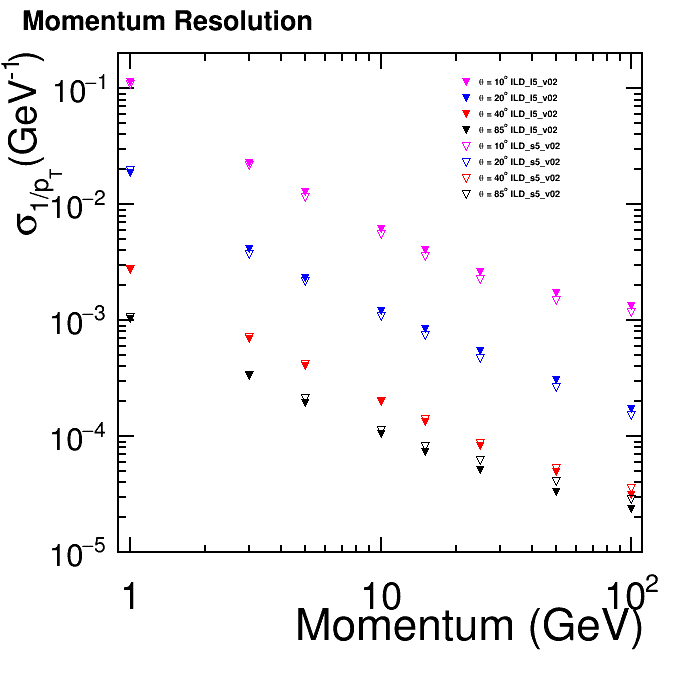
\includegraphics[width=\hsize]{Performance/fig/PResolution_compare_v02-00-02_New_ILD_ls5_v02.png}
 \caption{ \label{fig:perf:trk_pt}}
 \end{subfigure}
\begin{subfigure}{0.49\hsize} 
 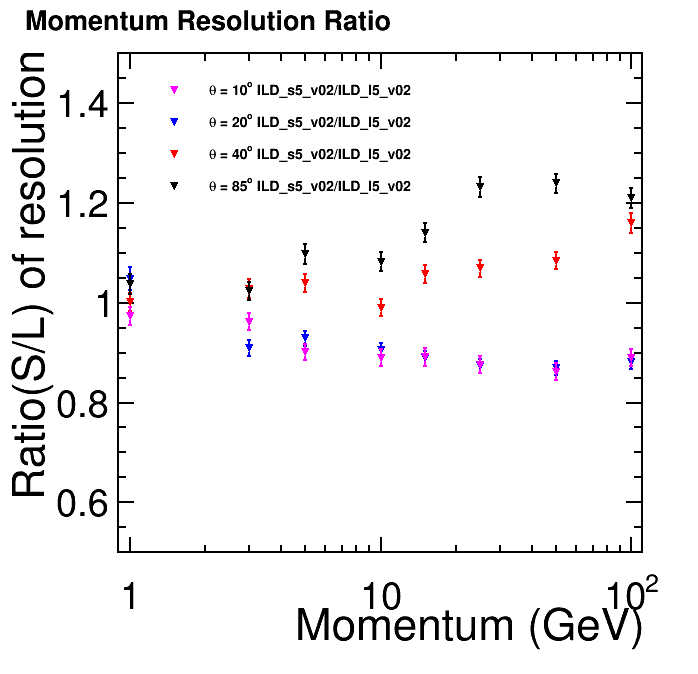
\includegraphics[width=\hsize]{Performance/fig/PResolution_Ratio_v02-00-02_New_ILD_ls5_v02.png}
 \caption{  \label{fig:perf:trk_ptcmp}}
 \end{subfigure}
\begin{subfigure}{0.49\hsize} 
 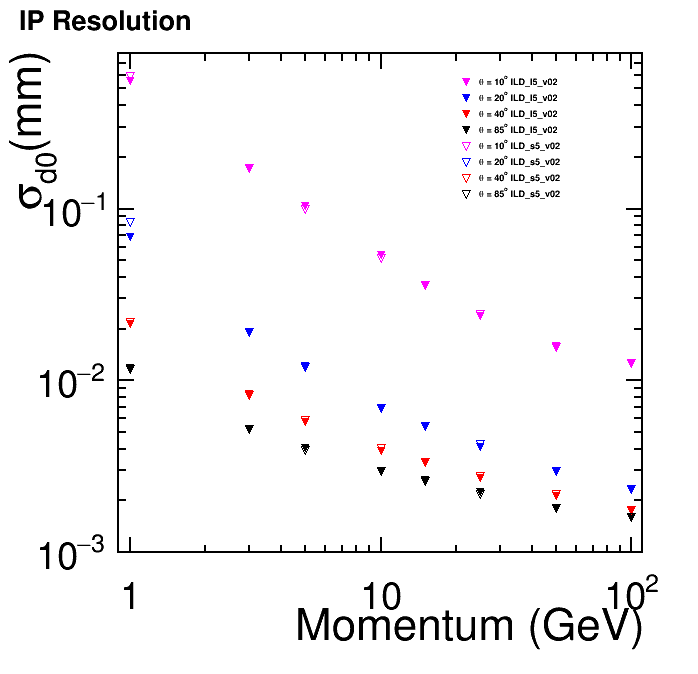
\includegraphics[width=\hsize]{Performance/fig/D0Resolution_compare_v02-00-02_New_ILD_ls5_v02.png}
 \caption{ \label{fig:perf:trk_d0}}
 \end{subfigure}
\begin{subfigure}{0.49\hsize} 
 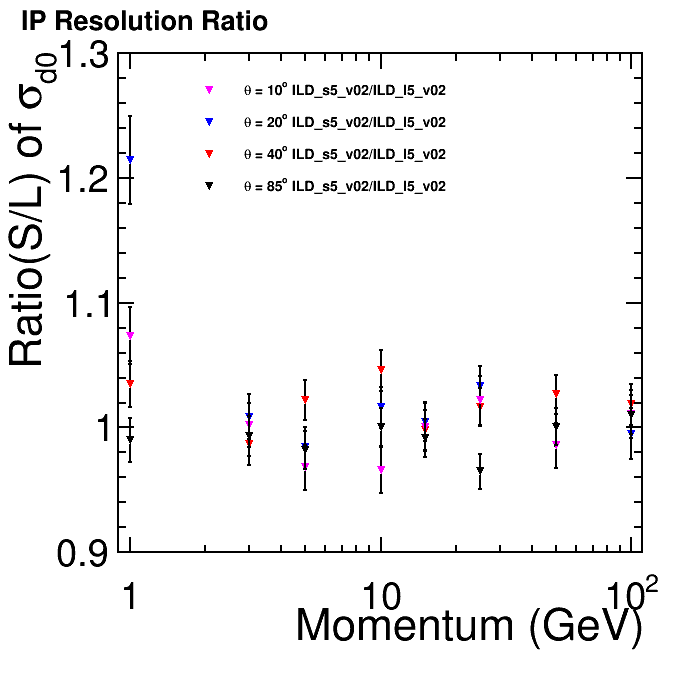
\includegraphics[width=\hsize]{Performance/fig/D0Resolution_Ratio_v02-00-02_New_ILD_ls5_v02.png}
 \caption{  \label{fig:perf:trk_d0cmp}}
 \end{subfigure}
\begin{subfigure}{0.49\hsize} 
 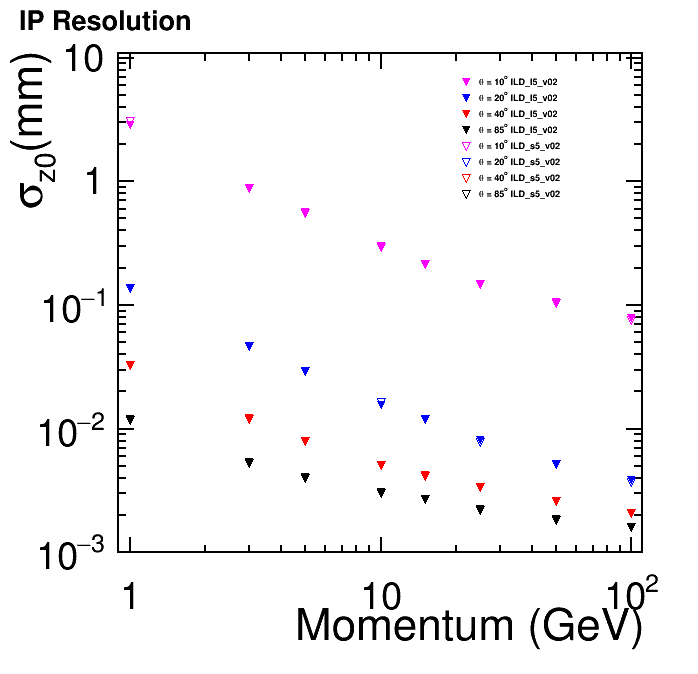
\includegraphics[width=\hsize]{Performance/fig/Z0Resolution_compare_v02-00-02_New_ILD_ls5_v02.png}
 \caption{ \label{fig:perf:trk_z0}}
 \end{subfigure}
\begin{subfigure}{0.49\hsize} 
 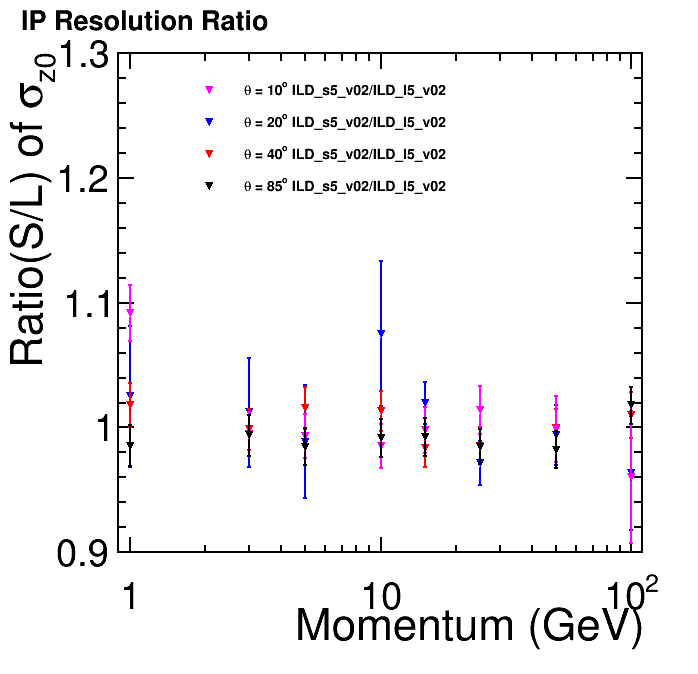
\includegraphics[width=\hsize]{Performance/fig/Z0Resolution_Ratio_v02-00-02_New_ILD_ls5_v02.png}
 \caption{  \label{fig:perf:trk_z0cmp}}
 \end{subfigure}
\caption{
  Tracking resolutions for single muons for the large and small ILD detector models.
  (a) Inverse transverse momentum resolution $\sigma_{1/p_T}$ as a function of momentum and the ratio $small/large$ in (b).
  (c) Impact parameter in the $r\phi$-plane $\sigma_{d0}$ as a function of momentum and the ratio $small/large$ in (d).
  (e) Impact parameter along the $z$-axis $\sigma_{z0}$  as a function of momentum and the ratio $small/large$  in (f).
}
\label{fig:perf:trkres}
\end{figure}

%
% % tracking efficiency for ttbar events
% 
\begin{figure}[htbp]
\begin{subfigure}{0.49\hsize} 
 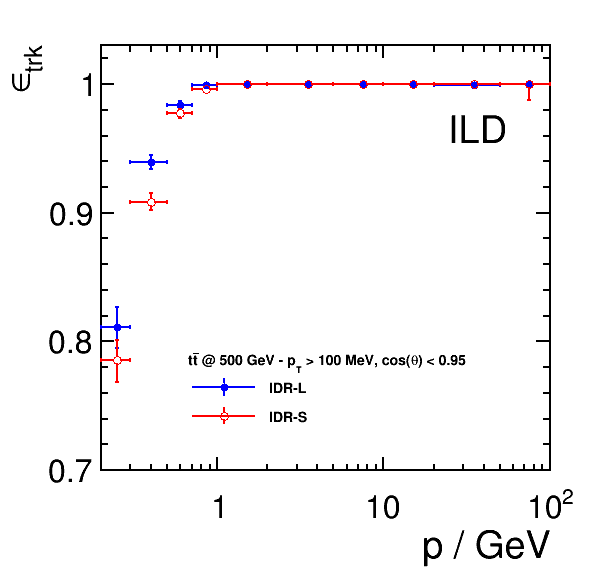
\includegraphics[width=\hsize]{Performance/fig/trkEff_p_ttbar_IDR.png}
 \caption{ \label{fig:perf:trkeff_p}}
 \end{subfigure}
\begin{subfigure}{0.49\hsize} 
 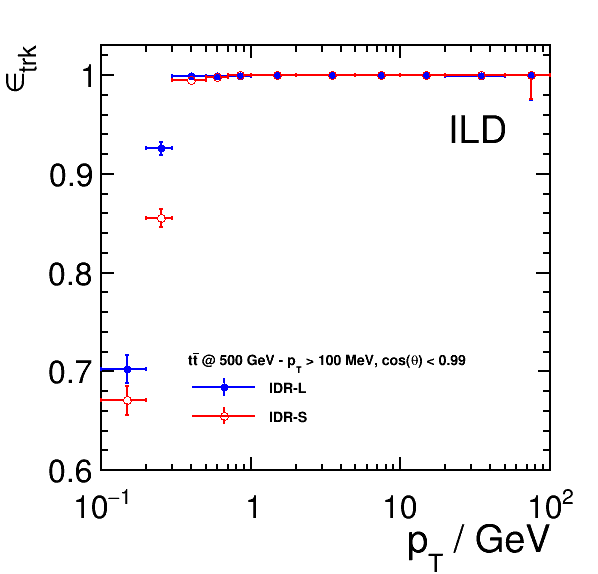
\includegraphics[width=\hsize]{Performance/fig/trkEff_pt_ttbar_IDR.png}
 \caption{  \label{fig:perf:trkeff_pt}}
 \end{subfigure}
\begin{subfigure}{0.49\hsize} 
 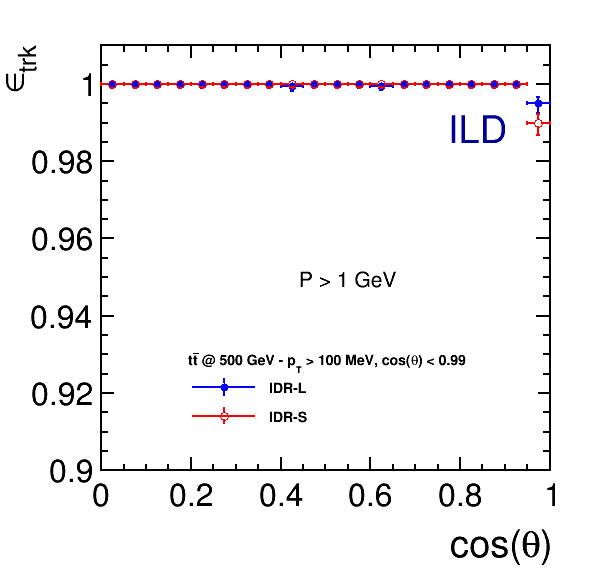
\includegraphics[width=\hsize]{Performance/fig/trkEff_th_ttbar_IDR.png}
 \caption{ \label{fig:perf:trkeff_th}}
 \end{subfigure}
\begin{subfigure}{0.49\hsize} 
 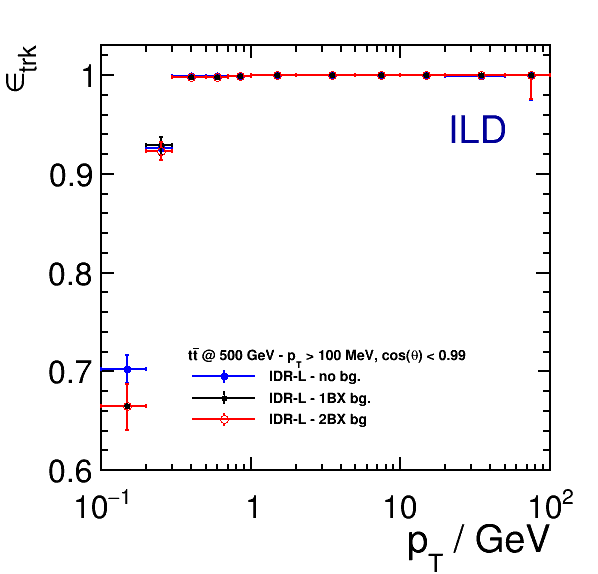
\includegraphics[width=\hsize]{Performance/fig/trkEff_pt_ttbar_pairBG_IDR.png}
 \caption{  \label{fig:perf:trkeff_bg}}
 \end{subfigure}
\begin{subfigure}{0.49\hsize} 
 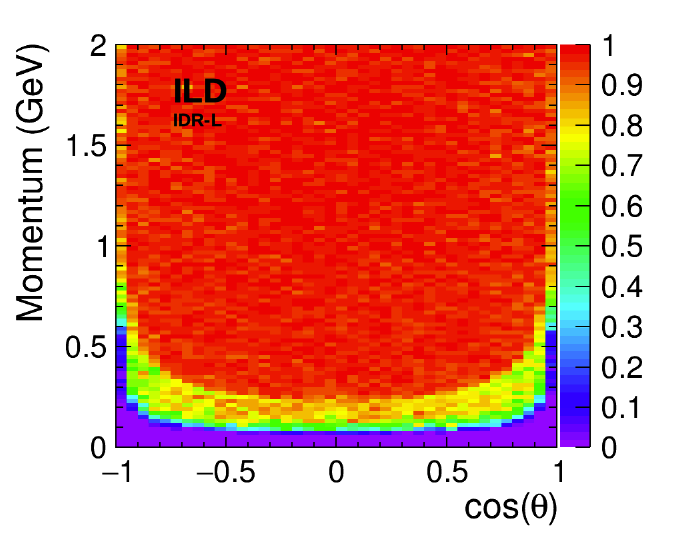
\includegraphics[width=\hsize]{Performance/fig/newSiliconTracking_10kEvents_effTrk_Momentum_v3.png}
 \caption{ \label{fig:perf:trkeff_2D_p}}
 \end{subfigure}
\begin{subfigure}{0.49\hsize} 
 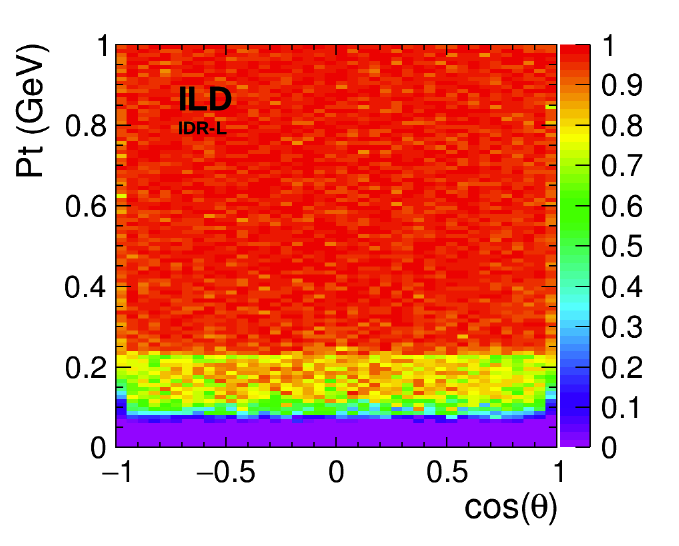
\includegraphics[width=\hsize]{Performance/fig/newSiliconTracking_10kEvents_effTrk_Pt_v3.png}
 \caption{  \label{fig:perf:trkeff_2D_pt}}
 \end{subfigure}
\caption{
  Track finding efficiency for prompt ($r_{vertex}<\unit{10}{\cm}$) tracks in $t \bar t$-events at 500 GeV as a function of kinematic variables for the large and small detector:
  (a) as a function of momentum $p$  (b) as a function of transverse momentum $p_T$ (c) as a function of $\cos(\theta)$).
  The effect on the efficiency of overlaying hits from 1BX and 2BX of pair background is shown in (d). The tracking efficiency as a
  function of $\cos(\theta)$ and either momentum or transverse momentum is shown for the large model in (e) and (f) respectively. 
}
\label{fig:perf:trkeff}
\end{figure}

The track finding efficiency of the algorithms described in section~\ref{sec:reco} is evaluated with $\Ptop\APtop$-events
at $E_{cms}=\unit{500}{\GeV}$ fully simulated and reconstructed for both detector models.
The tracking efficiency is defined as the ratio of the number of correctly reconstructed tracks with a hit purity higher than 75~\% to the
number of Monte Carlo tracks that are created within \unit{10}{\cm} of the {\em IP}, left at least 4 hits in the detector and
did not decay in flight. The resulting efficiency is shown in Fig.~\ref{fig:perf:trkeff} as a function of momentum $p$ in (a),
transverse momentum $p_T$ in (b) and $\cos(\theta$) in (c). As can be seen in (c), the tracking is almost perfect for particles
with $p>\unit{1}{\GeV}$ and $p_T>\unit{100}{\MeV}$ down to $\cos(\theta) \approx 0.95$ and better than 99~\% in the very forward
direction. At low momenta and in the forward direction, the small detector performs slightly worse than the larger variant, which
is due to the larger B-field that causes larger curvatures of the tracks. In the barrel region some of this effect could potentially
be alleviated by moving the innermost layer of the vertex closer to the beam, which would be possible as the background cone from
pair particles is also forced to lower radii by the higher B-field.

The qualitative dependency of the efficiency on momentum and polar angle together is shown in the 2D plots (e) and (f) for the large
detector model. The efficiency is basically flat as a function of transverse momentum in all but the very forward ($\cos(\theta)>0.95$)
part and almost perfect above $p_T>\unit{250}{\MeV}$ in that region. A small inefficiency persists in the very forward region
also for higher momenta. The above studies have been done with the same background overlaid as for the large Monte Carlo samples.
In (d) the tracking efficiency is shown also with complete and detailed simulations of one and two bunch crossings of pair
background overlaid. Only a very small degradation of the tracking efficiency at the lowest momenta is observed.

%%%%%%%%%%%%%%%%%%%%%%%%%%%%%%%%%%%%%%%%%%%%%%%%%%%%%%%%%%%%%%%
\subsection{Particle Flow performance and JER}
The performance of the Particle Flow Algorithm (PFA) is evaluated with dedicated  $\PZ\rightarrow \Pquark\APquark$-events, $\Pquark \in [\Pqu,\Pqd,\Pqs]$,
where the \PZ is chosen to have the desired mass of twice the jet energy and decays at rest. This allows to distinguish the measurement of the
actual jet energy resolution (JER) from other effects like ISR-photons or confusion in jet clustering that occur in more complex,
realistic events.
%
% JER and JES for uds,c,b events
% 
\begin{figure}[htbp]
\begin{subfigure}{0.49\hsize}
 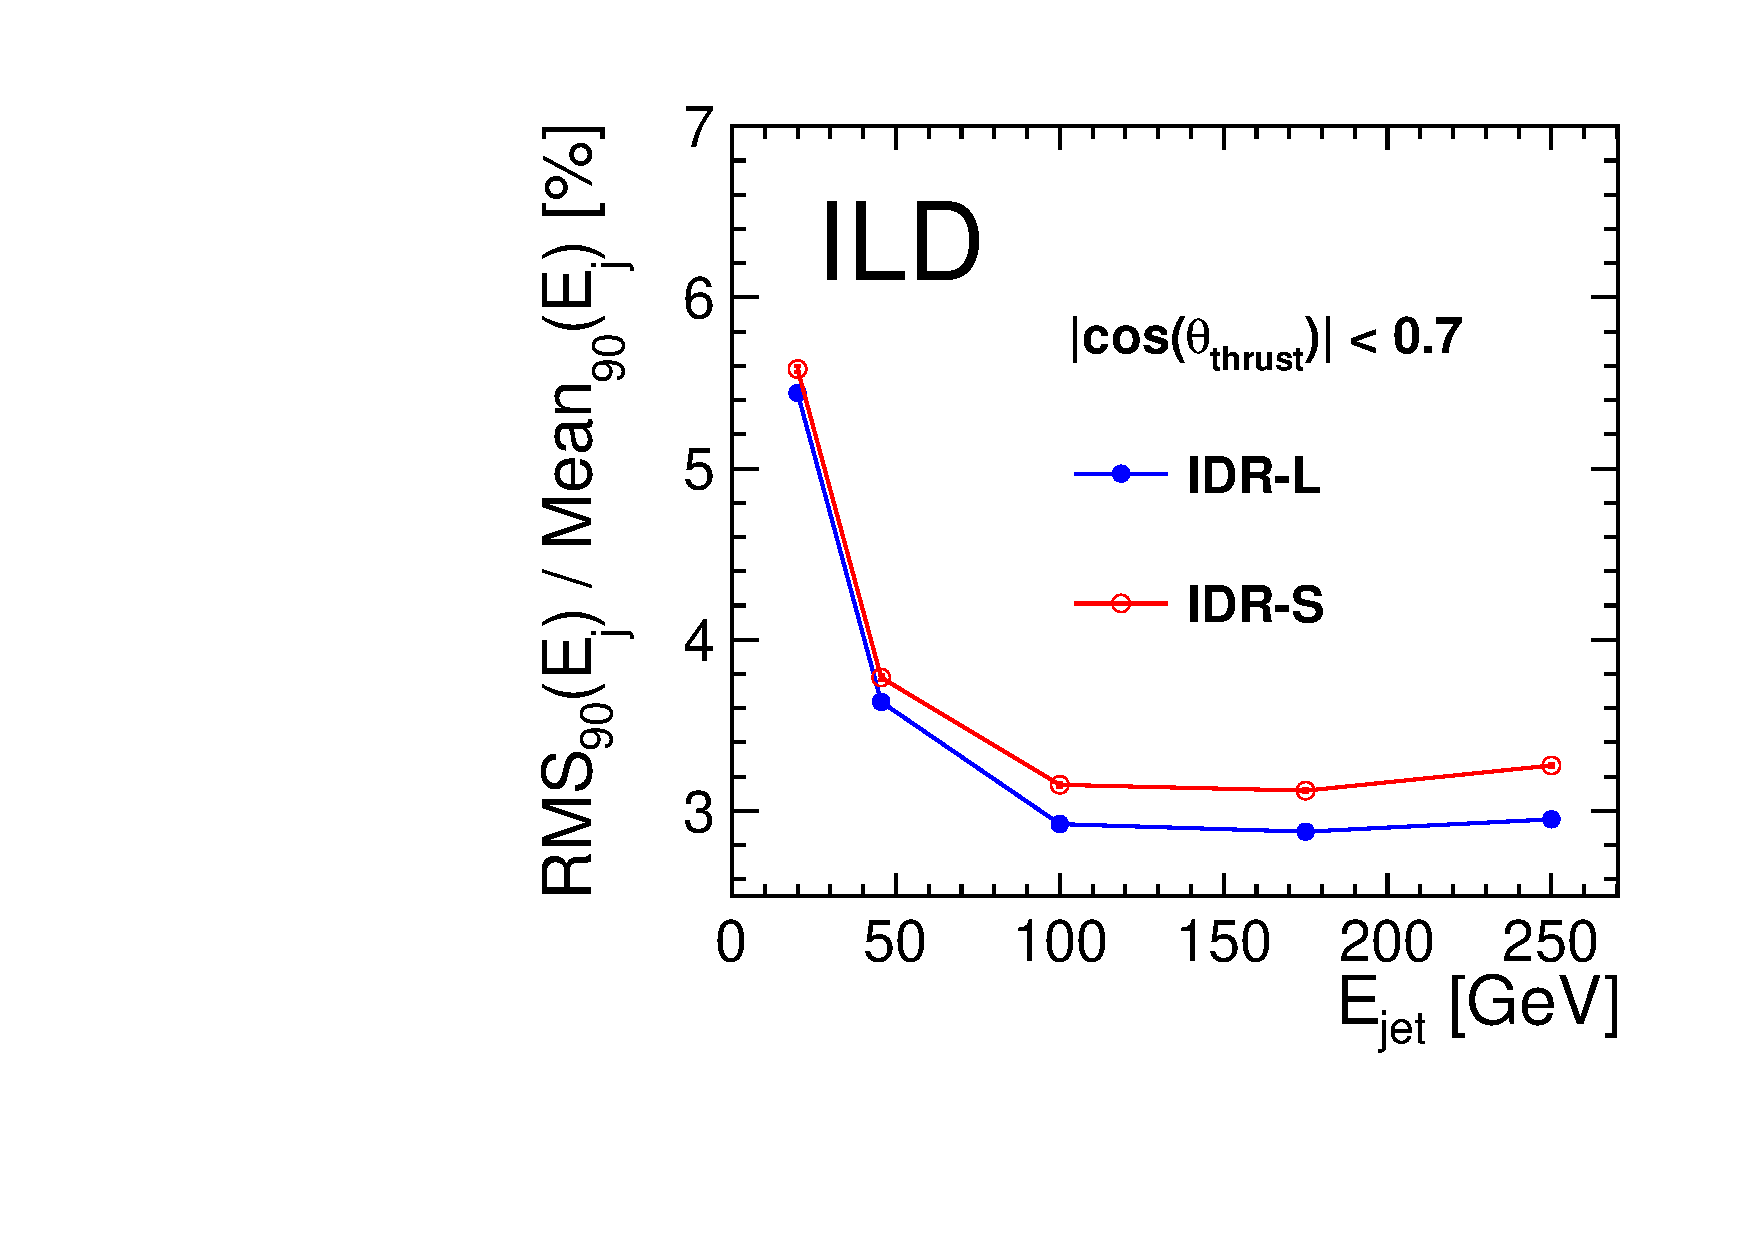
\includegraphics[width=\hsize]{Performance/fig/JERs_uds_l5_vs_s5_Barrel.pdf}
 \caption{ \label{fig:perf:pfa_jer}}
 \end{subfigure}
\begin{subfigure}{0.49\hsize}
 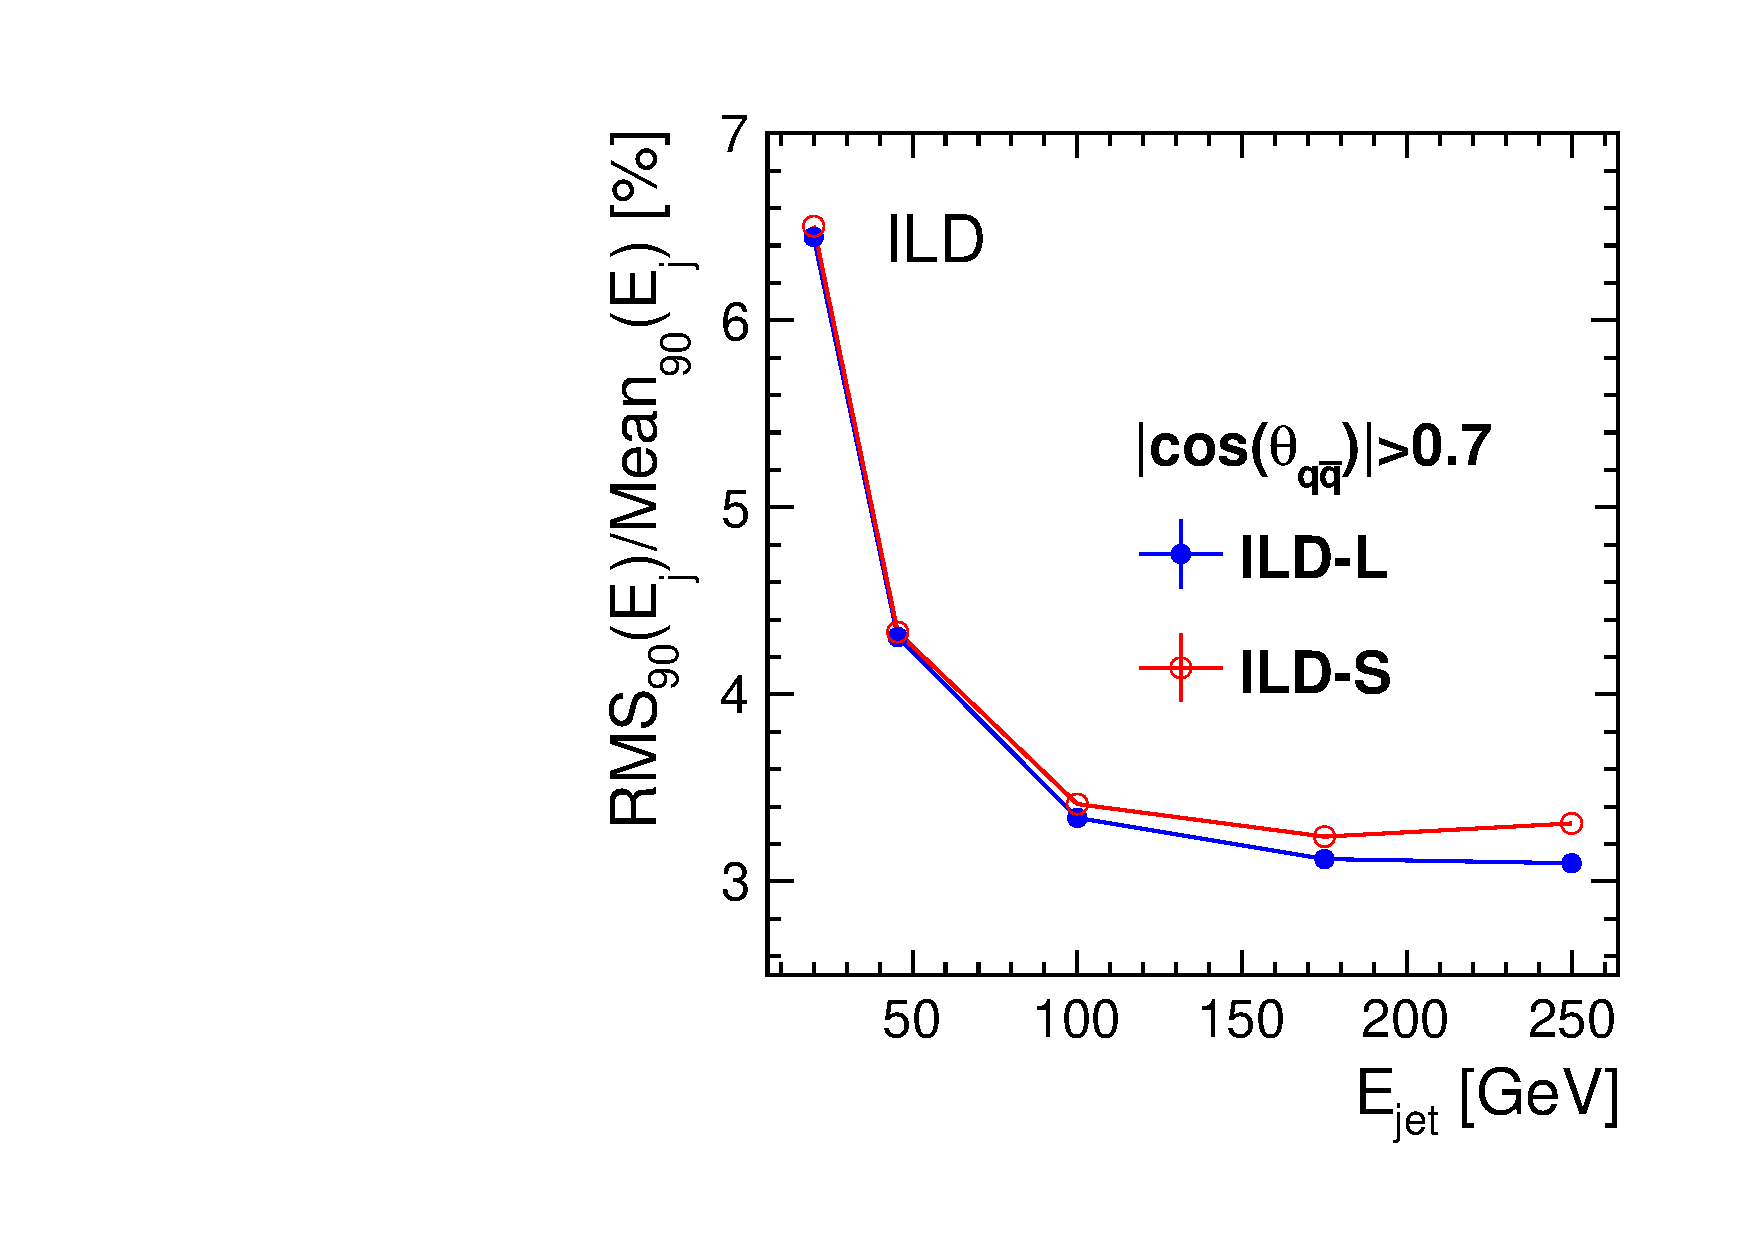
\includegraphics[width=\hsize]{Performance/fig/JERs_uds_l5_vs_s5_Endcap.pdf}
 \caption{  \label{fig:perf:pfa_jer_endcap}}
 \end{subfigure}
\begin{subfigure}{0.49\hsize}
 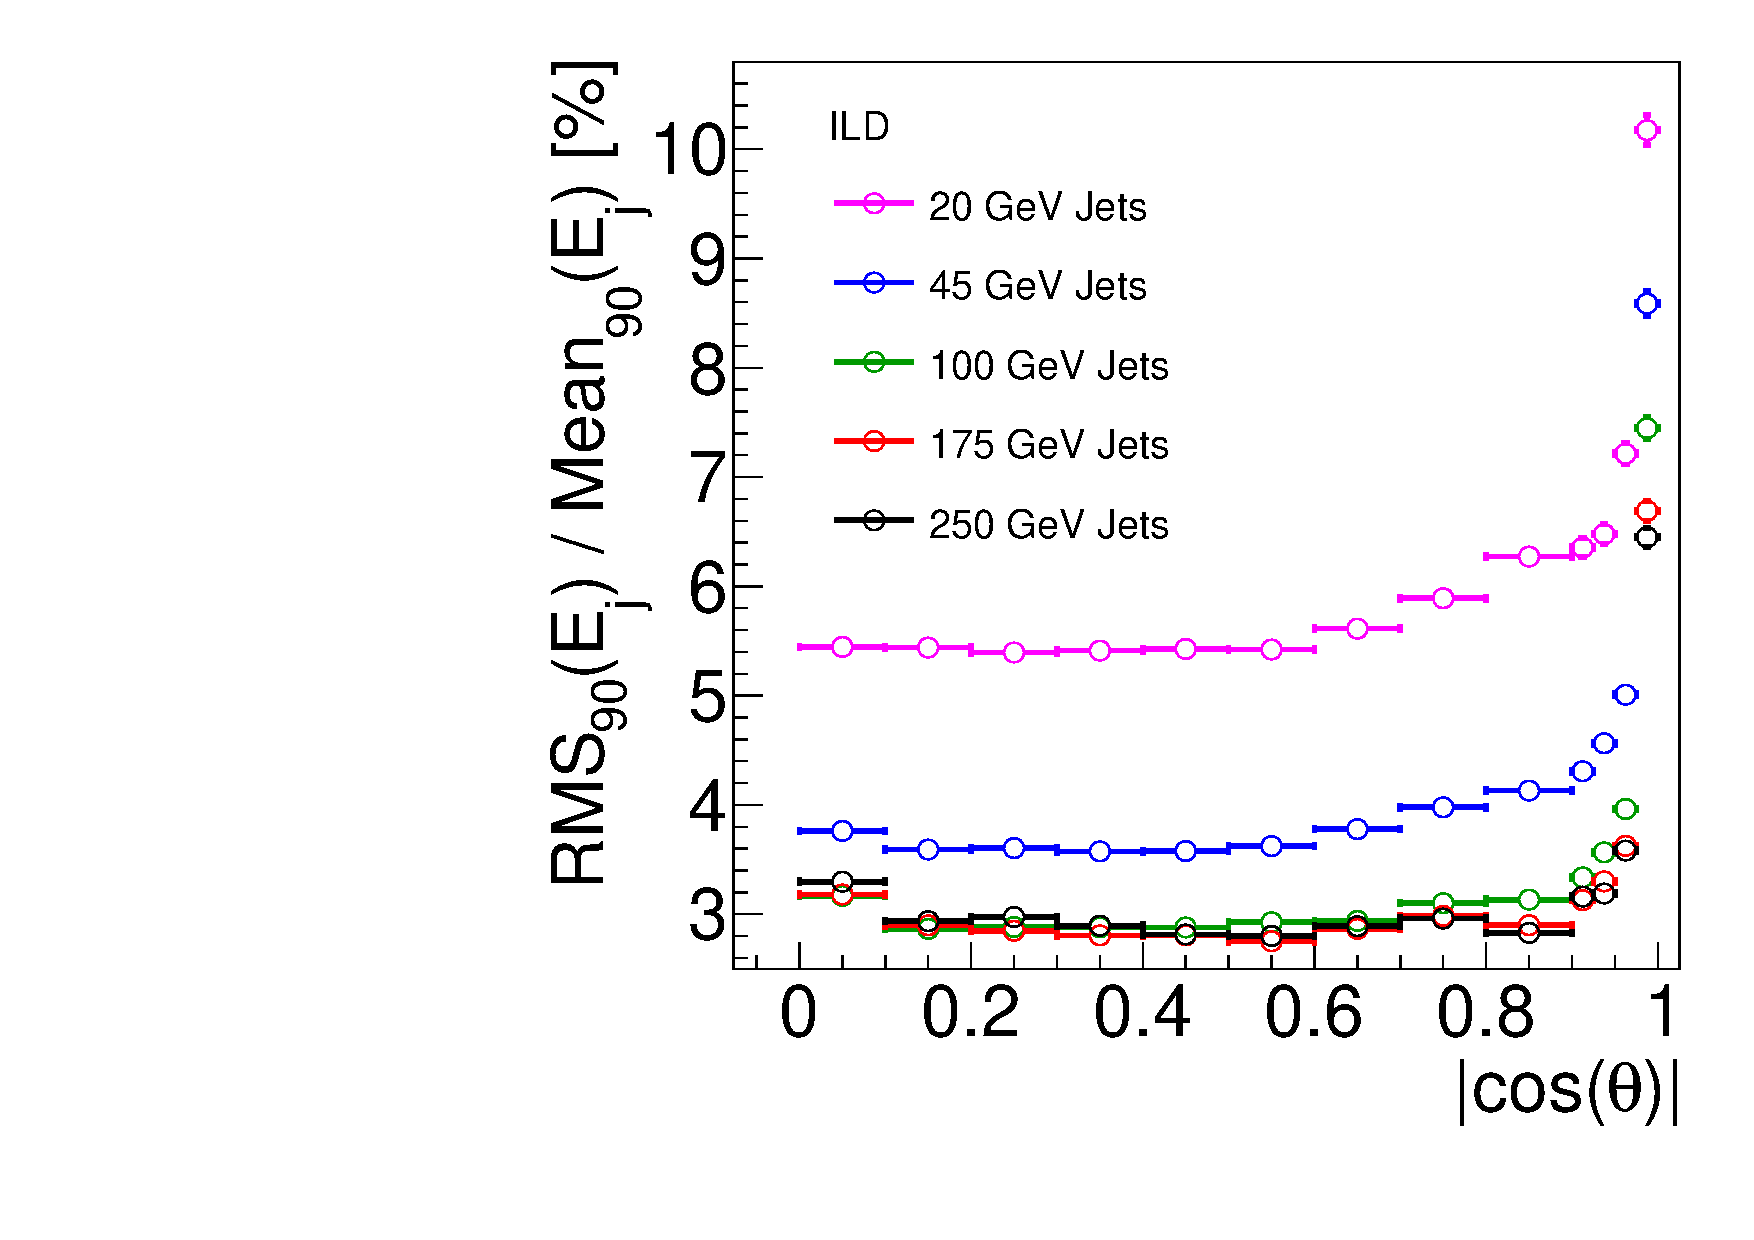
\includegraphics[width=\hsize]{Performance/fig/JER_vs_cosTheta.pdf}
 \caption{ \label{fig:perf:pfa_costh}}
 \end{subfigure}
\begin{subfigure}{0.49\hsize}
 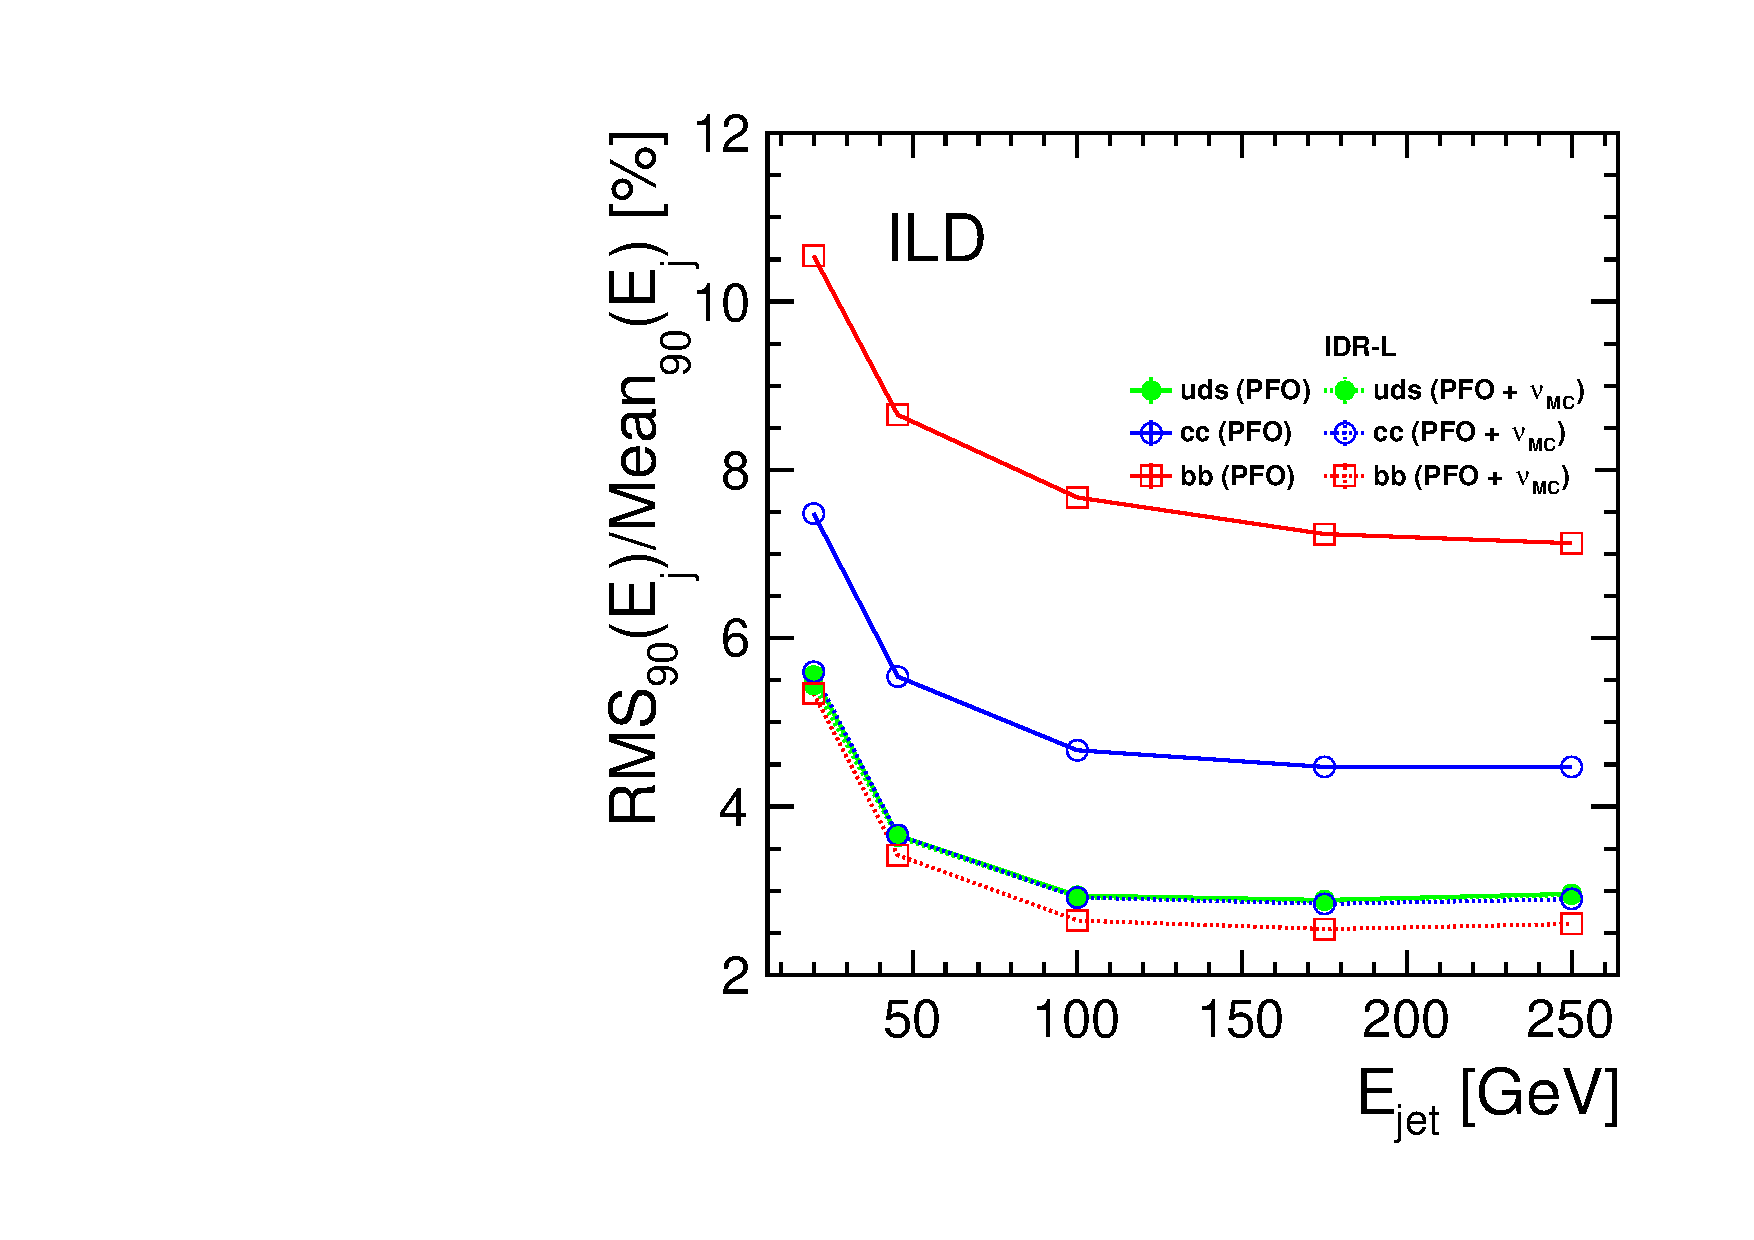
\includegraphics[width=\hsize]{Performance/fig/JERs_bcuds_pfo_vs_pfo_plus_nu.pdf}
 \caption{  \label{fig:perf:pfa_udscb}}
 \end{subfigure}
\begin{subfigure}{0.49\hsize}
 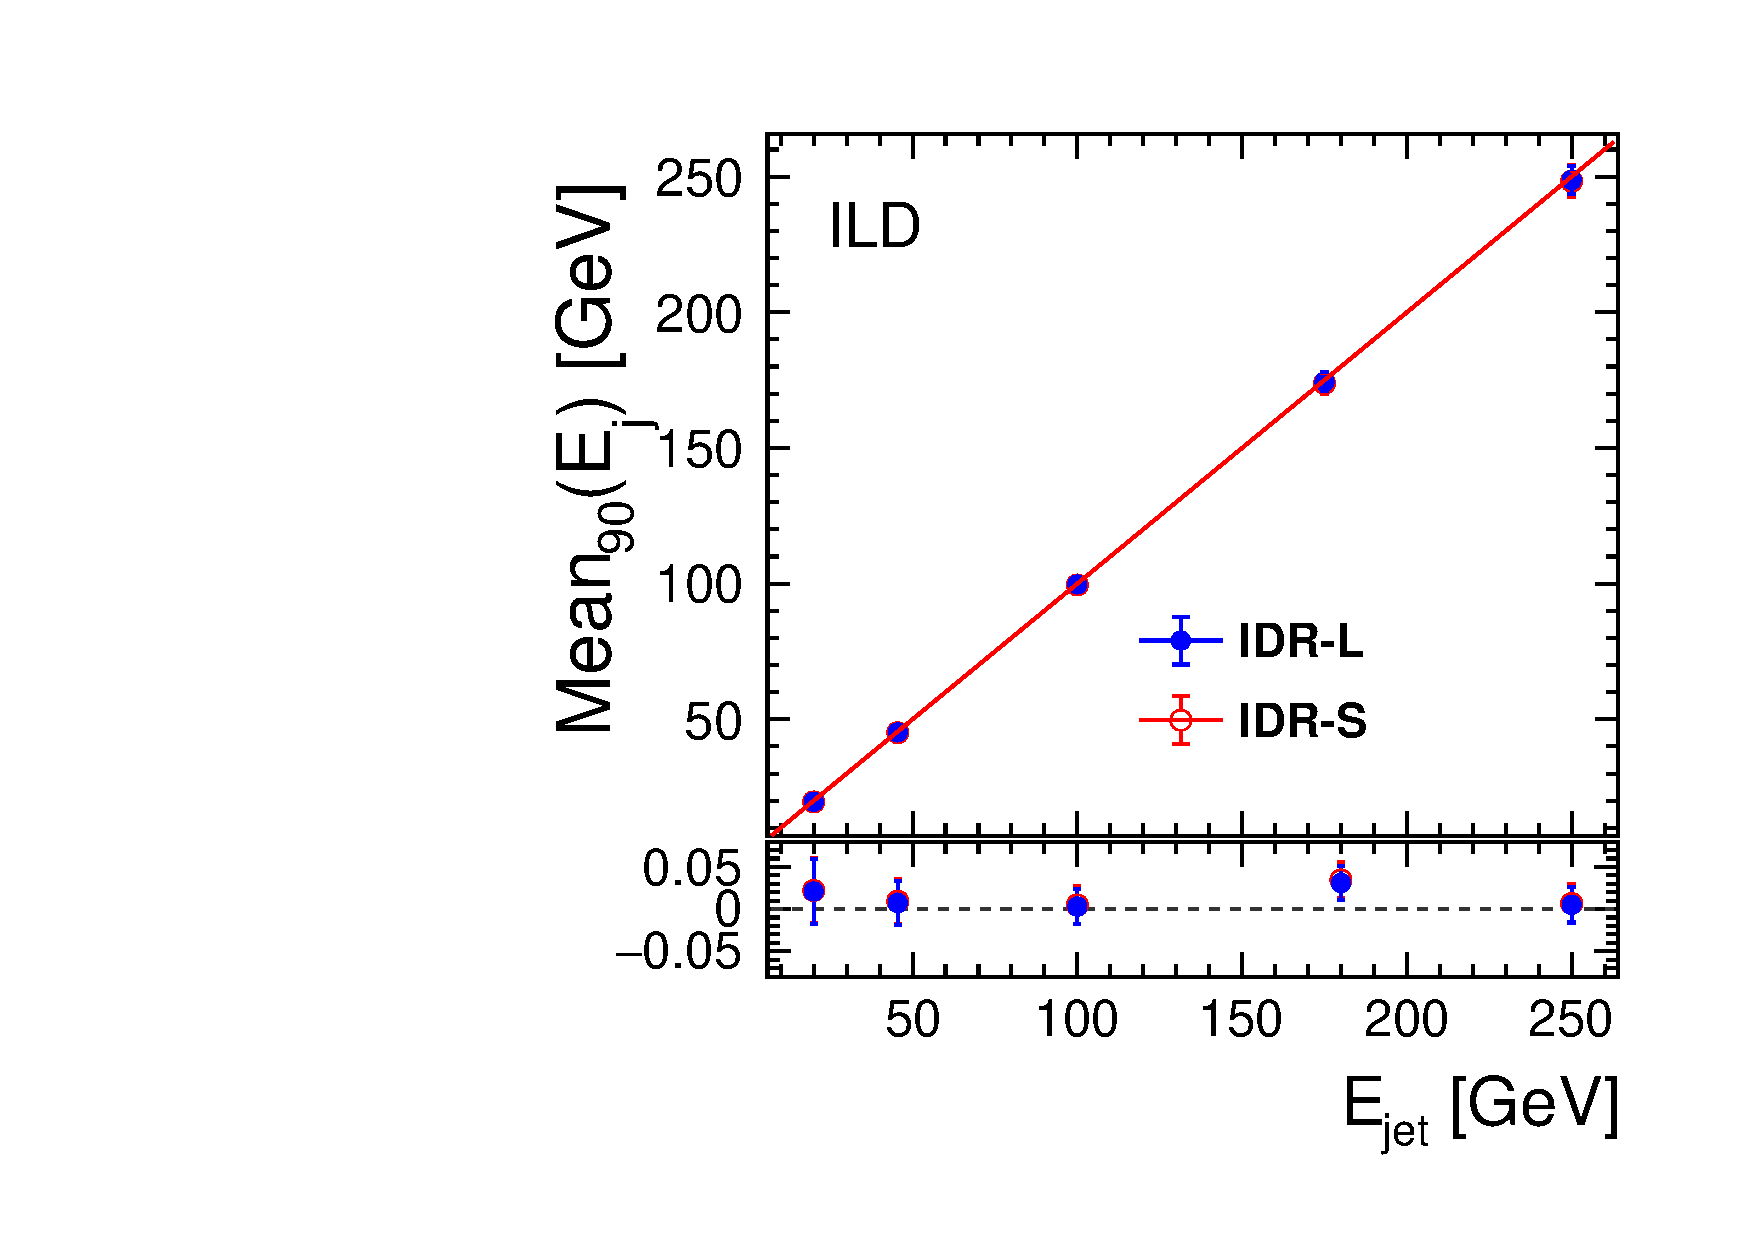
\includegraphics[width=\hsize]{Performance/fig/JESs_uds_l5_vs_s5.pdf}
 \caption{  \label{fig:perf:pfa_jes}}
 \end{subfigure}
\caption{
  Jet energy resolution (JER), evaluated as defined in eq.~\ref{ild:eq:jer} for $\PZ\rightarrow \Pquark\APquark$-events and $\Pquark \in [\Pqu,\Pqd,\Pqs]$.
  (a) comparison of the JER for the large and small ILD detector in the barrel region with
  $|\cos(\theta_{thrust})|<0.7$  (b) the same for the endcap region with  $0.7<|\cos(\theta_{thrust})|<0.98$
  (c) JER as function of the polar angle ({\em thrust}-axis) of the event. (d) JER for $\Pqu,\Pqd,\Pqs$ di-jet events together with $\Pqc\APqc$ and $\Pqb\APqb$ events,
  with (dashed lines) and without (solid lines) correcting the $\Pneutrino$ energies using Monte Carlo truth information. (e) Jet energy scale for the large and small model
  for barrel events.
  }
\label{fig:perf:pfa}
\end{figure}
%
%
The jet energy resolution is then evaluated as 
\begin{equation}\label{ild:eq:jer}
\frac{ \sigma_{E_{jet}} } { E_{jet}}  :=  \frac{\rmsn(E_{jet})}{ \mathrm{mean}_{90}(E_{jet})}
\end{equation}
%%%for $\PZ\rightarrow \Pquark\APquark$-events with $|\cos(\theta_{q\bar q})|<0.7$ and $\Pquark \in [\Pqu,\Pqd,\Pqs]$.
The $\rmsn$ is defined to be the $rms$ of the central $90\%$ of the distribution and the $\mathrm{mean}_{90}$ is its mean value.
This measure is robust against large tails and
should be multiplied by a factor of $\sim1.1$ to obtain an equivalent Gaussian analyzing power\cite{ild:bib:PandoraPFA}.
Fig.~\ref{fig:perf:pfa_jer} shows the JER as a function of the jet energy for selected energies $E_{jet}=\unit{(20, 45, 100, 175, 250)}{\GeV}$
for the large and small detector model in the barrel region ($|\cos(\theta_{thrust})|<0.7$) . For $E_{jet}\geq \unit{45}{\GeV}$ the resolution is better than 4\% and
approaches 3\% (3.2\%) for the large (small) model at higher energies. In the forward region ($|\cos(\theta_{thrust})|>0.7$) the JER is
slightly worse and the difference between large and small detector is less pronounced as can bee seen in Fig.~\ref{fig:perf:pfa_jer_endcap}. In order to
ensure that the jets are fully contained in the acceptance of the detector, an additional cut of  $|\cos(\theta_{thrust})|<0.98$ is applied.
The JER as a function of the polar angle of the jets (the {\em thrust}-axis of the di-quark events) is shown in Fig.~\ref{fig:perf:pfa_costh} for the
large detector model. The observed dependency is rather flat throughout the barrel region, increasing somewhat after the barrel-end-cap transition
with a visible rise in the very forward region, similar for all energies. The effect of heavy flavor quarks on the jet energy resolution is shown in
Fig.~\ref{fig:perf:pfa_udscb}, where the resolutions is plotted for $\Pqu,\Pqd,\Pqs$ di-quark events together with $\Pqc\APqc$ and $\Pqb\APqb$ events for the large model.
The observed degradation in the JER for the heavy quark jets can be fully attributed to the missing energy carried by neutrinos,
as can be seen from the dashed lines, were the energy is corrected for the $\Pneutrino$~-energies using Monte Carlo truth information.
The linearity of the jet energy measurement is shown in Fig.~\ref{fig:perf:pfa_jes} to be better than 5\% in the barrel region.


%%%%%%%%%%%%%%%%%%%%%%%%%%%%%%%%%%%%%%%%%%%%%%%%%%%%%%%%%%%%%%%
\subsection{Vertexing}

The correct identification of heavy flavour decays in jets requires a precise measurement of the coordinates of secondary vertices.
The vertex resolution is studied with the dedicated $\Pep\Pem \rightarrow 6~\Pqc$ events that are also used for the flavour tagging
training and performance studies, described in section~\ref{sec:perf:hlr:lcfi}.
%
The resolution is measured along the longitudinal direction of the jet $\vec{e}_L$
and two transverse directions $\vec{e}_{T1}$ and $\vec{e}_{T2}$, defined as:
%
\begin{equation}
\vec{e}_L = \frac{ \vec{p}_c }{|\vec{p}_c| }~; ~~~~~~~  \vec{e}_{T1} = \vec{e}_L \times \vec{z} ~; ~~~~~~~  \vec{e}_{T2} = \vec{e}_L \times \vec{e}_{T1}
\end{equation}
whith the 3-momentum of the $\Pqc$-quark $\vec{p}_c$ taken from Monte Carlo truth.
The result is shown for the transverse (a) and longitudinal (b) components of the secondary vertices as a function of the distance from the $IP$
in Fig.~\ref{fig:perf:vtxres}.
\begin{figure}[htbp]
\begin{subfigure}{0.49\hsize}
 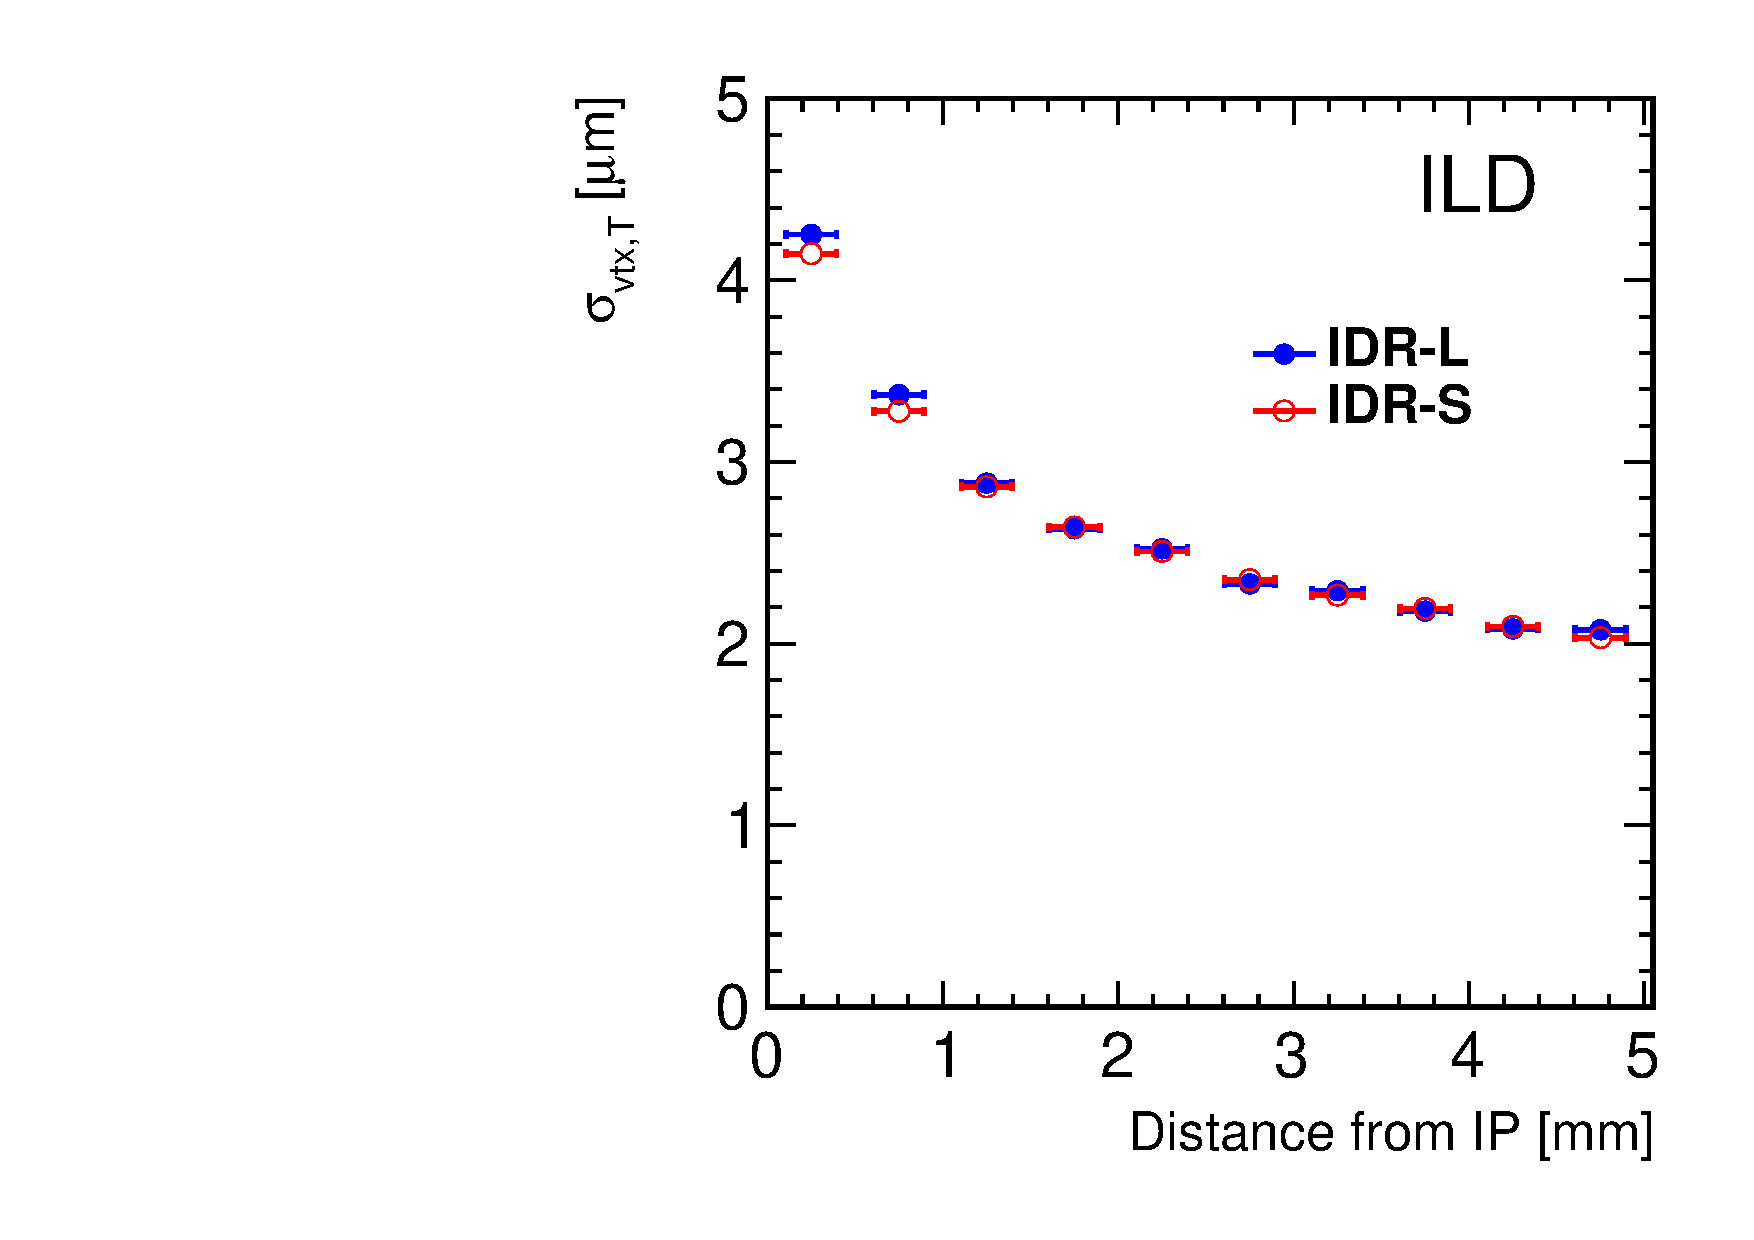
\includegraphics[width=\hsize]{Performance/fig/svtx_r_resol.pdf}
 \caption{ \label{fig:perf:svtx_r}}
 \end{subfigure}
\begin{subfigure}{0.49\hsize}
 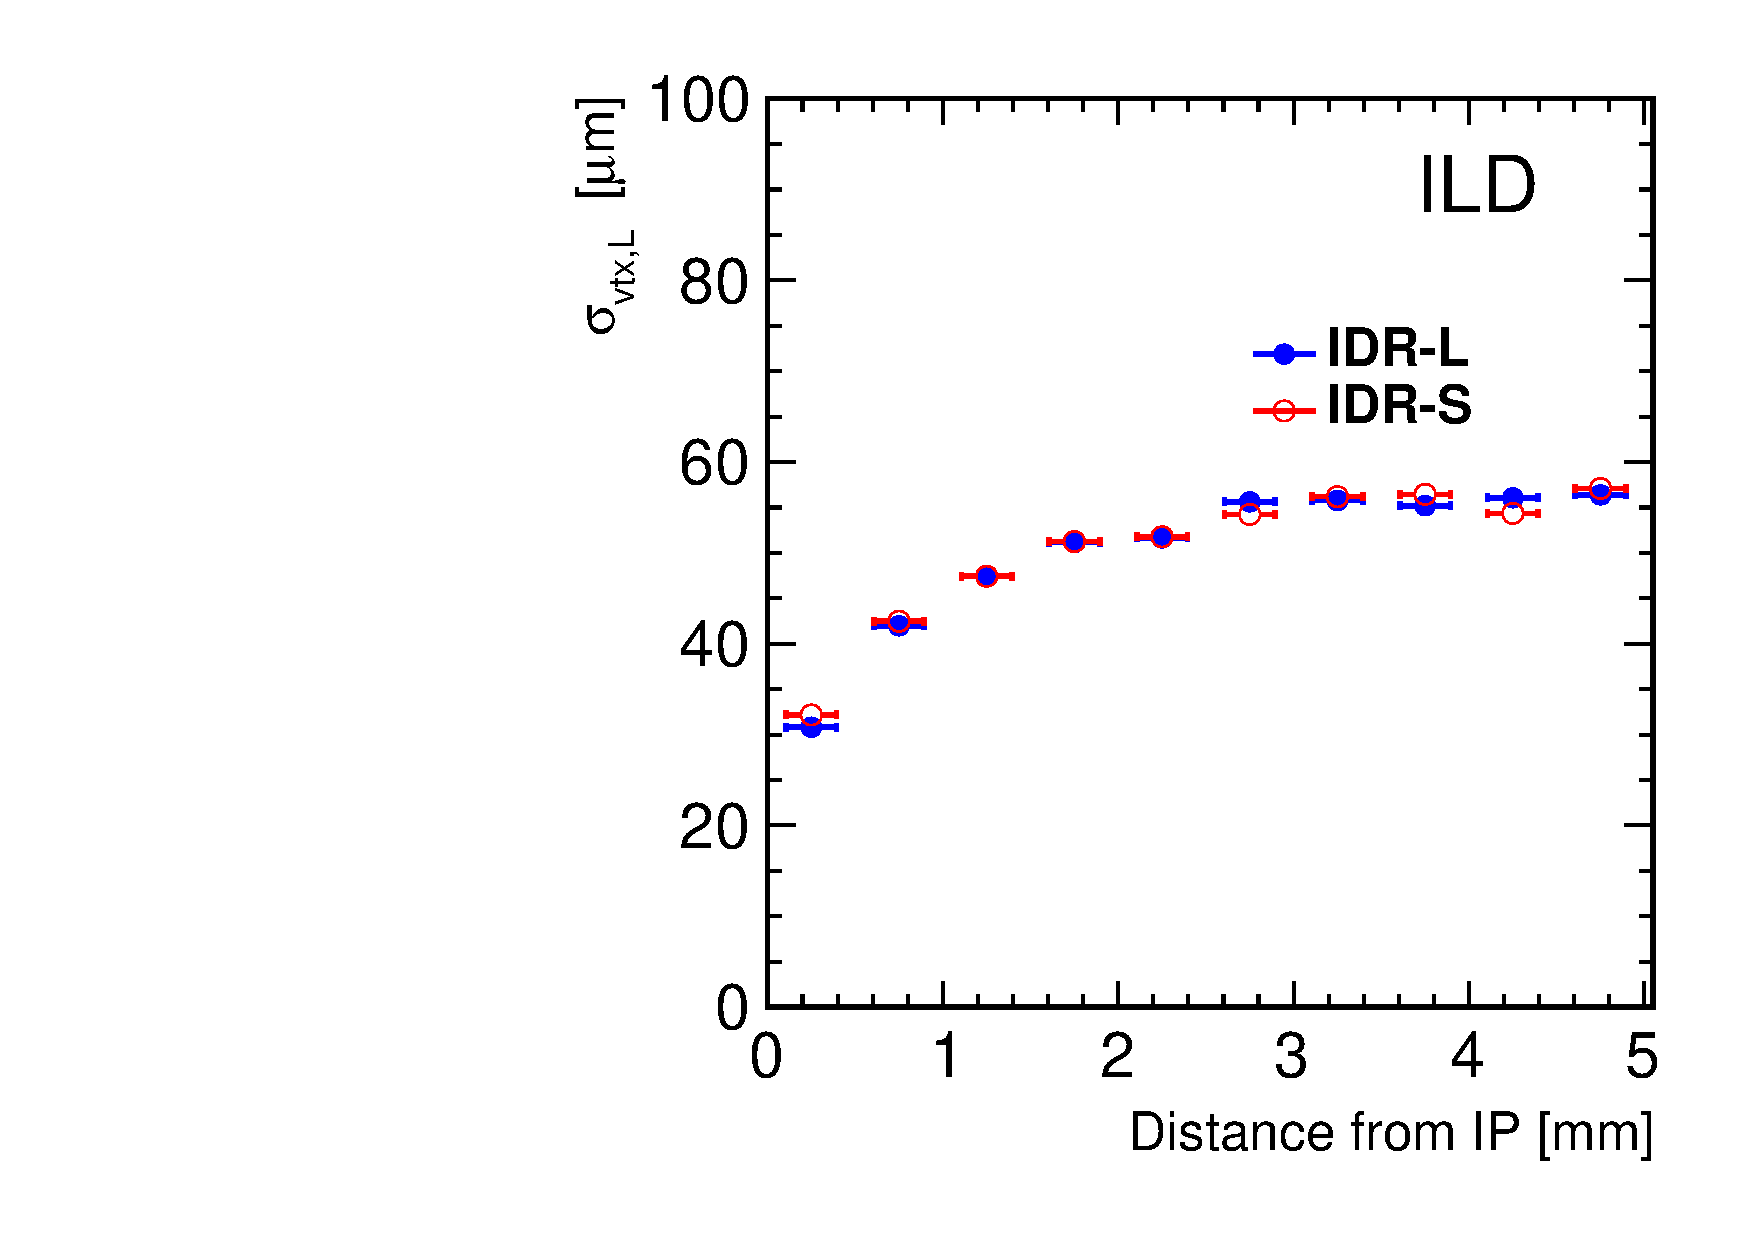
\includegraphics[width=\hsize]{Performance/fig/svtx_z_resol.pdf}
 \caption{  \label{fig:perf:svtx_z}}
 \end{subfigure}
\begin{subfigure}{0.49\hsize}
 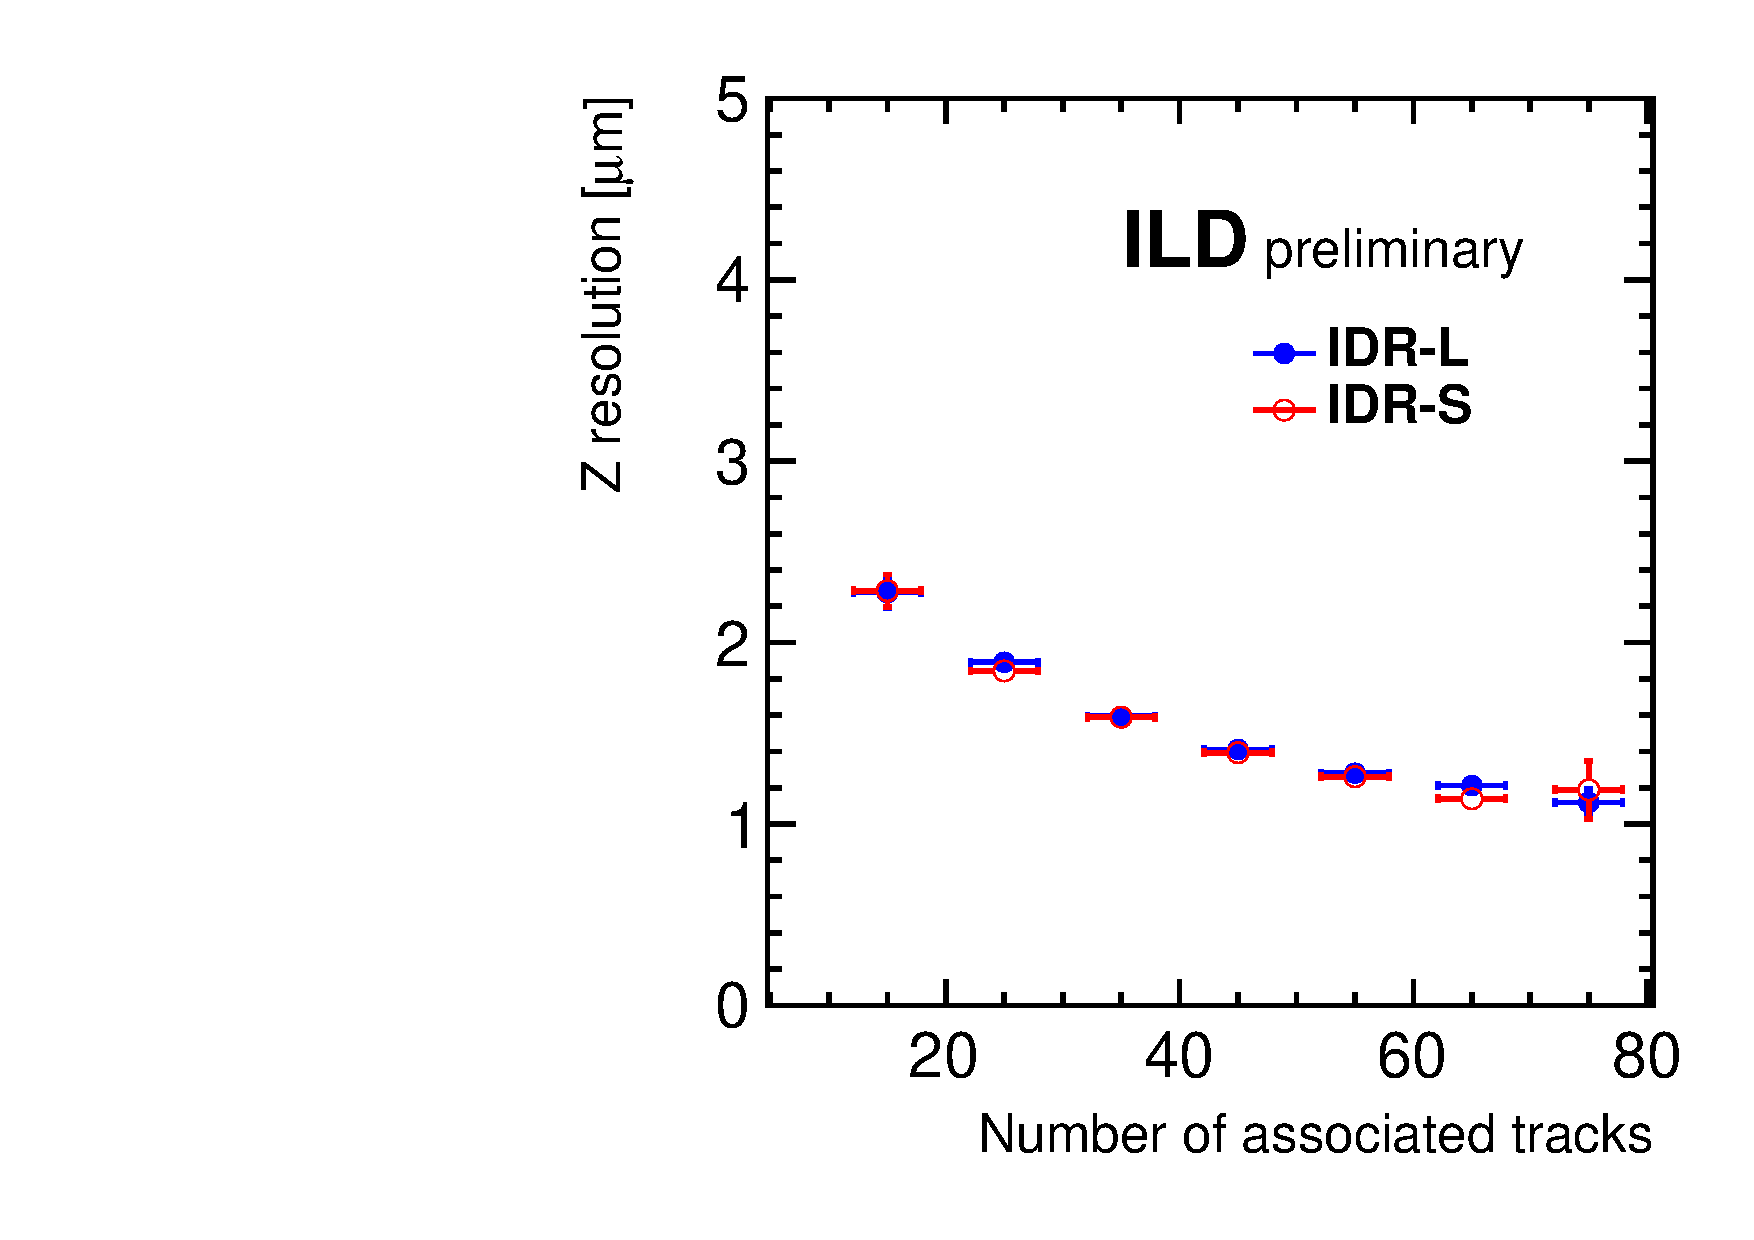
\includegraphics[width=\hsize]{Performance/fig/pvtx_z_resol.pdf}
 \caption{  \label{fig:perf:pvtx_z}}
 \end{subfigure}
\caption{ Vertex resolutions for the large and small ILD detector models for  $\Pep\Pem \rightarrow 6~\Pqc$ events at $\sqrt{s}=\unit{500}{\GeV}$.
  (a) Resolution of the transverse component of secondary vertices as a function of the distance from the $IP$ and the same for the longitudenal component in (b).
  (c) Resolution of the z-coordinate of the primary vertex as a function of the number of tracks used in the fit. 
  Note that the radial component of the primary vertex is known extremely well to \unit{O(10)}{\nm} from the beam-spot position.
}
\label{fig:perf:vtxres}
\end{figure}
%
Fig.~\ref{fig:perf:pvtx_z} shows the resolution of the primary vertex' z-position as a function of the number of associated tracks.
The resolution is better than \unit{3}{\micron} for low multiplicity events and
approaches \unit{1}{\micron} for high multiplicity events.  The radial component of the primary vertex is already known
extremely well from the beam-spot position to \unit{O(10)}{\nm}. The overall vertexing performance for the large and small detector models
is very similar, as expected already from the single track impact parameter resolutions shown in Fig.~\ref{fig:perf:trkres} (c)-(f).



%%%%%%%%%%%%%%%%%%%%%%%%%%%%%%%%%%%%%%%%%%%%%%%%%%%%%%%%%%%%%%%
%%\subsection{Photon Reconstruction}
%%\fix{no publishable results for photon ID available ...}
%%%%%%%%%%%%%%%%%%%%%%%%%%%%%%%%%%%%%%%%%%%%%%%%%%%%%%%%%%%%%%% 
%%\subsection{Lepton ID}
%%\fix{muons, electrons - no publishable results for lepton ID available ...}
%%%%%%%%%%%%%%%%%%%%%%%%%%%%%%%%%%%%%%%%%%%%%%%%%%%%%%%%%%%%%%%
\subsection{Charged Particle identification}
%\fix{dE/dx, potentially ToF, shower shapes}
%
%
Measuring the energy loss of charged particles in the ILD-TPC provides a powerful tool for identifying the type of the particle.
%%\thisfloatsetup{floatwidth=\SfigwFull,capposition=below}
\begin{figure}[htbp]
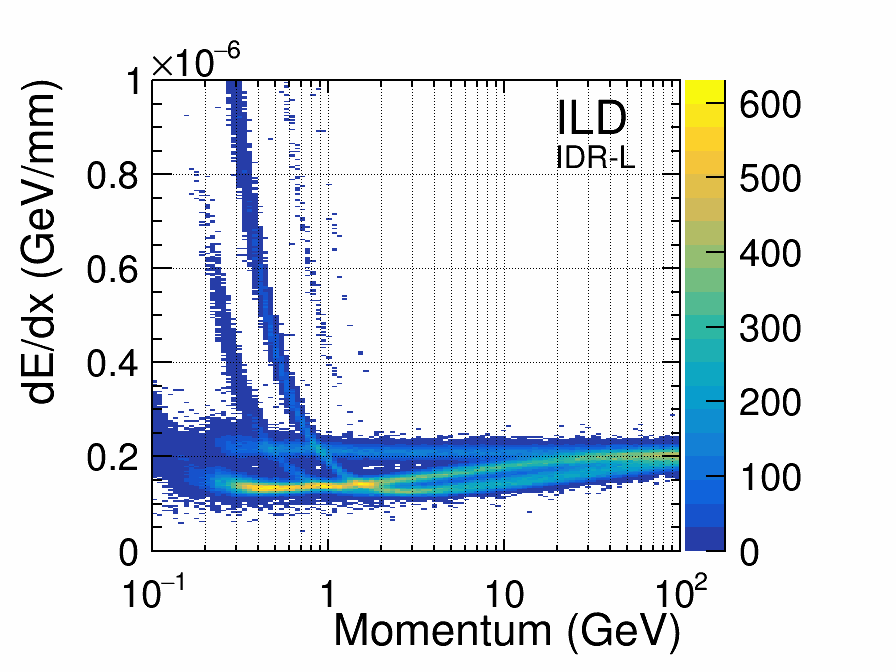
\includegraphics[width=0.8\hsize]{Performance/fig/dEdx_BBAll_lowGran_bigCap.png}
\caption{\label{fig:perf:dedx_tpc}
  $dE/dx$ as a function of particle momentum as reconstructed from a full simulation of single particle events ($\Pe, \Pmu, \Ppi, \PK$ and $\Pproton$)
  in the TPC of the large ILD detector model. The particles were simulated with a logarithmic momentum distribution and isotropic direction. Spurious
  entries in the bands for more massive particles, such as the deuteron, as well as entries from low momentum particles, below the TPC acceptance,
  are due to secondaries created in the events.
}
\end{figure}
%
Fig.~\ref{fig:perf:dedx_tpc} shows the $dE/dx$ reconstructed from a truncated mean for charged particle tracks in the TPC as a function of
the particle momentum, clearly revealing the bands of the most abundant particle types $\Pepm, \Pmupm, \Ppipm, \PKpm$ and $p^{\pm}$.
By fitting Gaussian distributions, with mean $\mu(p)$ and standard deviation $\sigma(p)$, to individual bands in momentum bins one can
define a separation power $\eta_{A,B}$ for distinguishing the two particle types A and B:
\begin{equation}
\eta_{A,B}(p) = \frac{ |\mu_A(p) - \mu_B(p)| } { \sqrt{ \frac{1}{2} ( \sigma^2_A(p) + \sigma^2_B(p) )  }  }
\label{ild:eq:seppow}
\end{equation}
Figure~\ref{fig:perf:dedxtof} shows the separation power
for $\Ppi,\PK$ and $\PK,\Pp$  based on the $dE/dx$ measurement in the TPC of the large and small detector model (a)
and the possible improvement that could be achieved by combining it with a  {\em time-of-flight (TOF)} measurement in the large detector (b).
As a proof of concept a possible TOF estimator is computed here. It uses the first ten calorimeter hits in the Ecal that are closest to the straight line,
resulting from extrapolation of the particle's momentum into the calorimeter, assuming an individual time resolution of $100$~ps
per hit\footnote{While this time resolution seems realisticly possible, it has to be noted, that so far it has not yet been demonstrated
 in a test beam prototype.}. The results optained clearly motivate further studies on timing measurements and optimised TOF estimators
in the ILD calorimeters.
%
% dE/dx separation power - combined w/ TOF
% 
\begin{figure}[htbp]
\begin{subfigure}{0.49\hsize}
 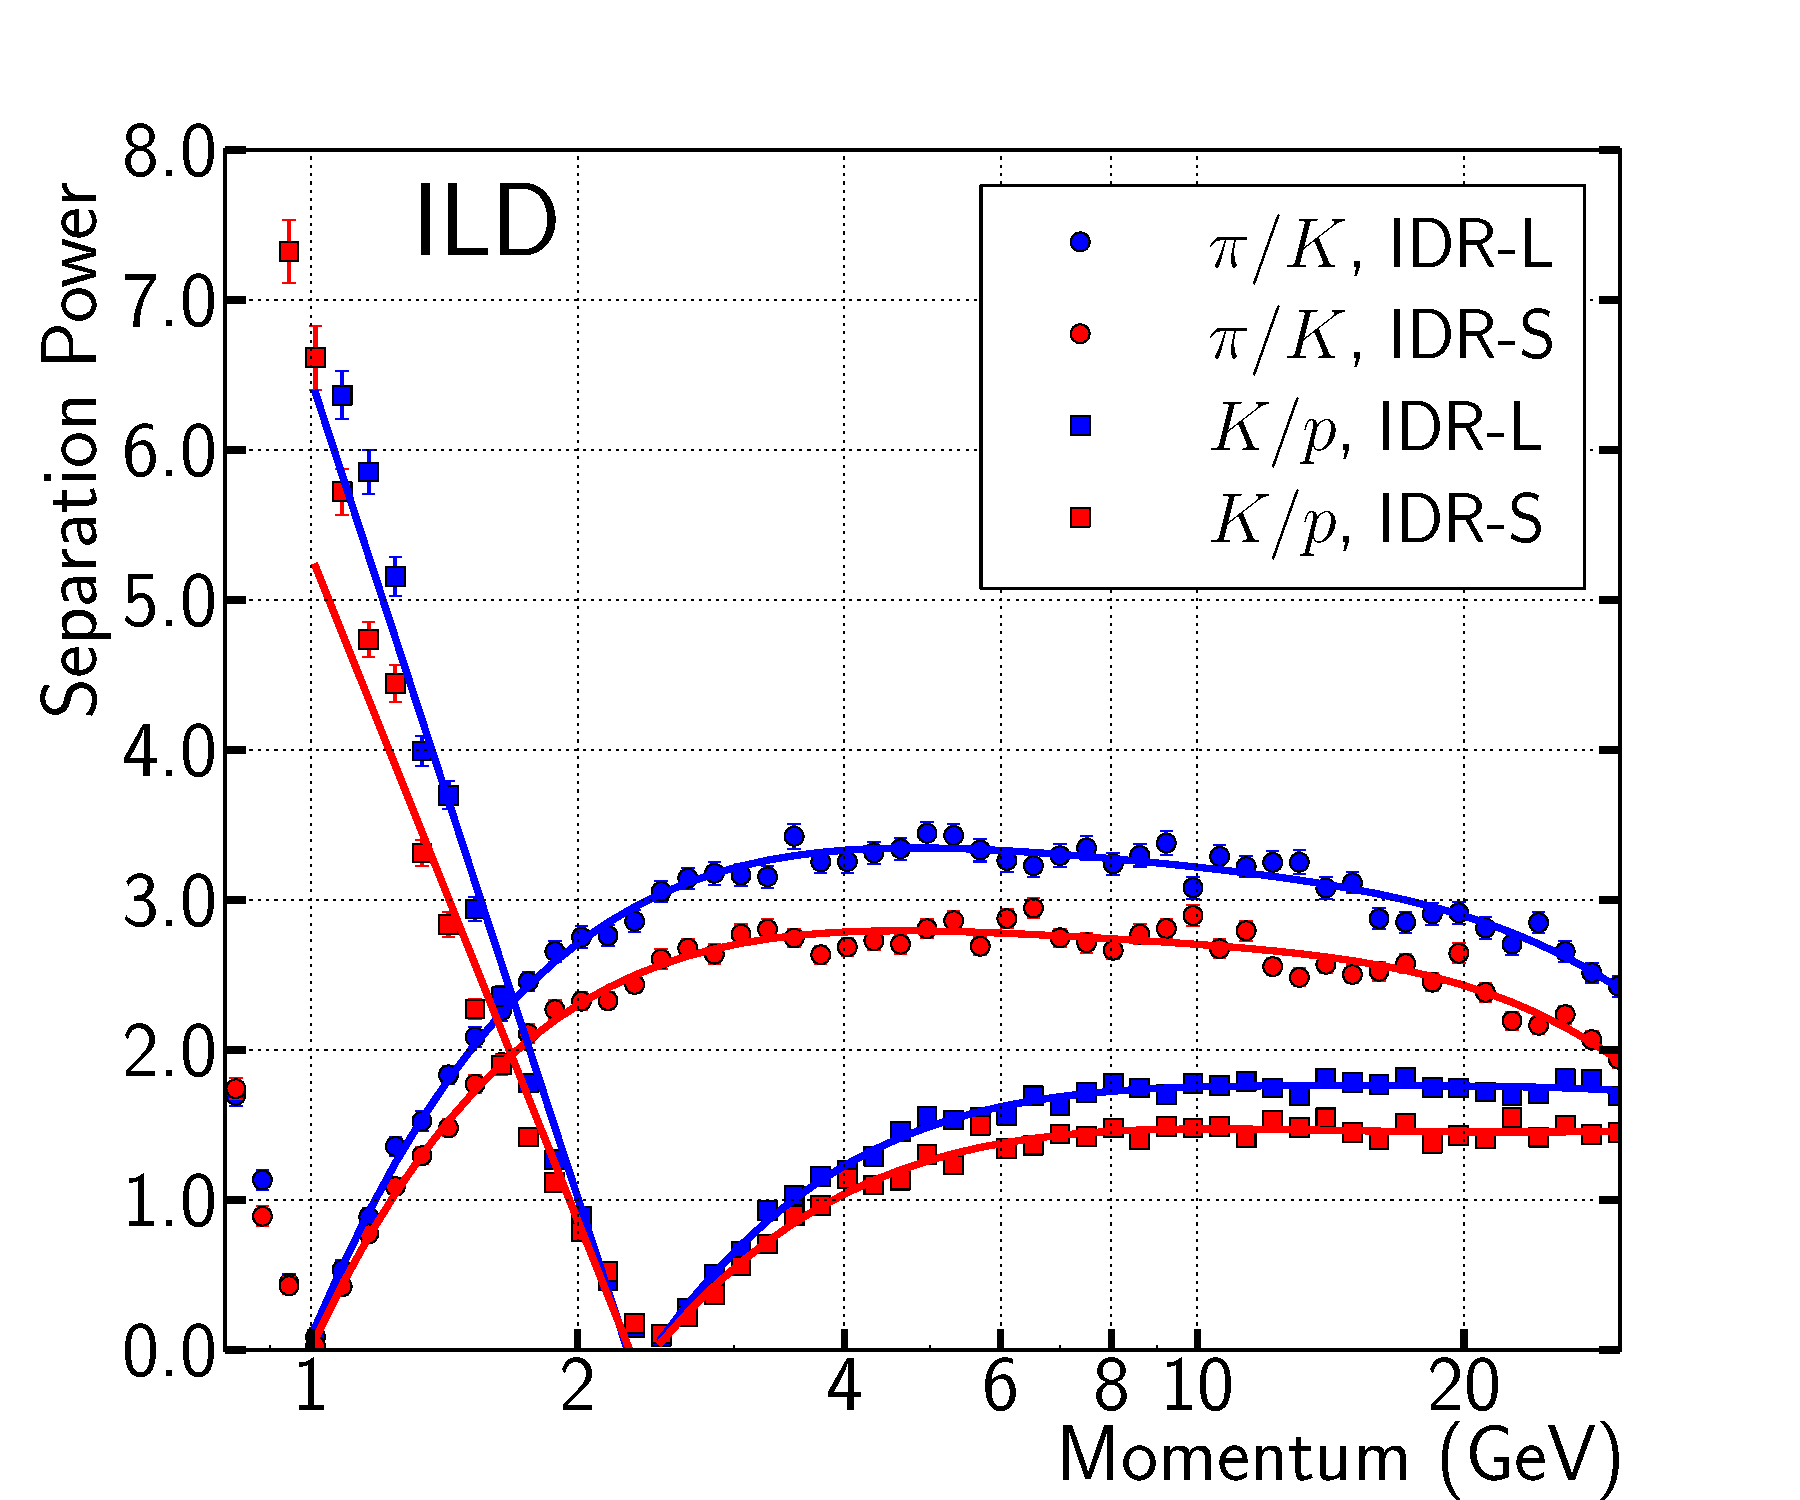
\includegraphics[width=\hsize]{Performance/fig/dEdx_ILDls_separation_power.pdf}
 \caption{ \label{fig:perf:dedx_sep}}
 \end{subfigure}
\begin{subfigure}{0.49\hsize}
 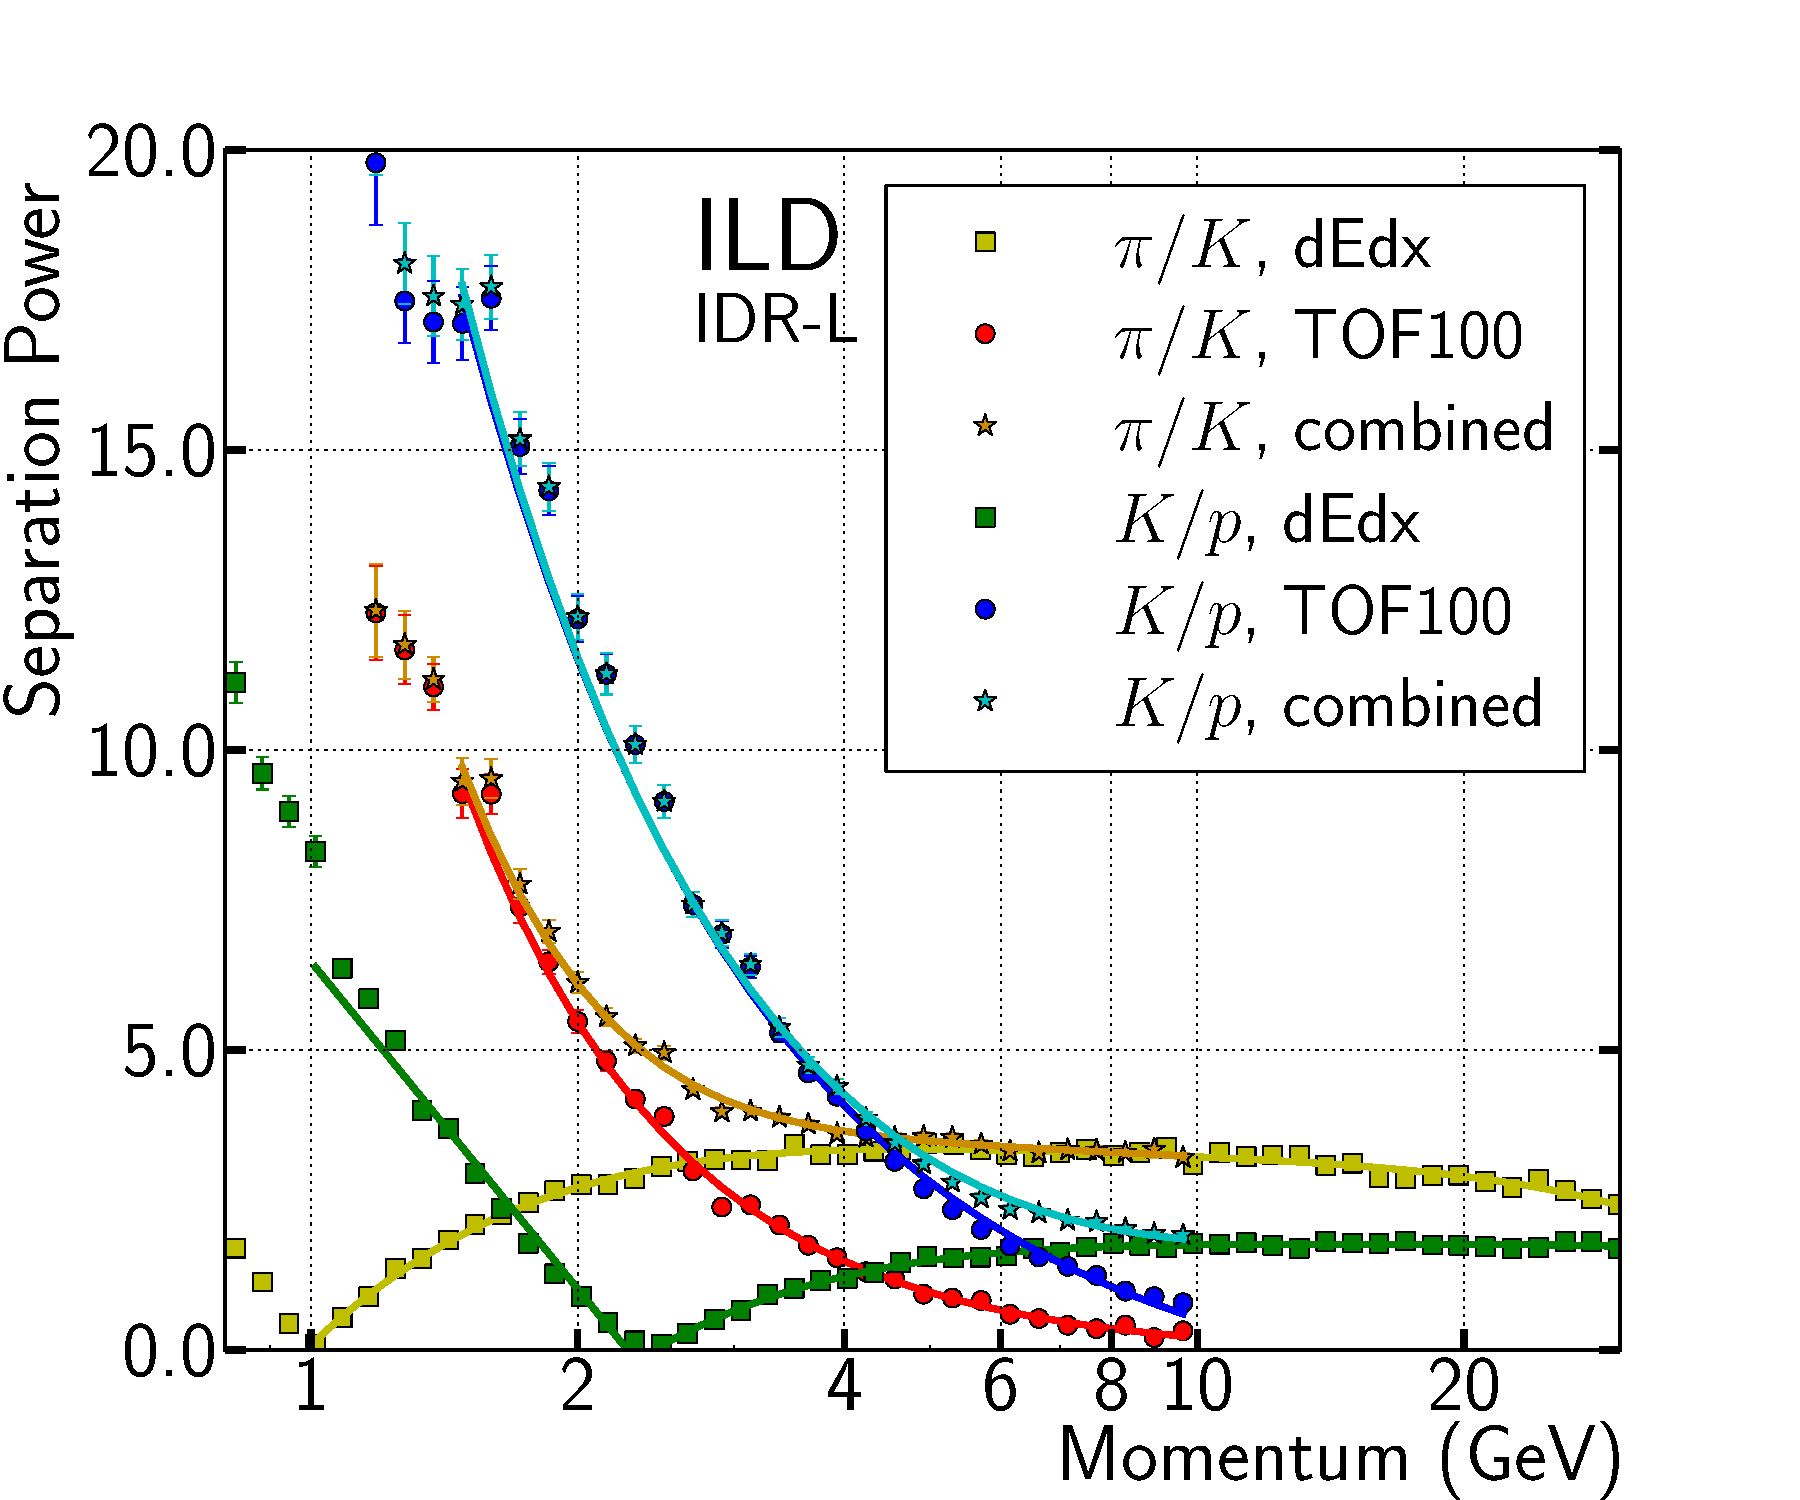
\includegraphics[width=\hsize]{Performance/fig/Combined_dEdx_TOF100_HiStat.pdf}
 \caption{  \label{fig:perf:dedxtof_sep}}
 \end{subfigure}
\caption{ (a) particle separation power (eq.~\ref{ild:eq:seppow}) for $\Ppi/\PK$ and $\PK/\Pp$ based on the $dE/dx$ measurement in the TPC.
  (b) improvement of the same separation power if combined with a {\em time-of-flight (TOF)} estimator from the first ten Ecal layers,
  where $\eta_{dE/dx,TOF}=\eta_{dE/dx} \oplus \eta_{TOF}$. The curves are shown to guide the eye.
}
\label{fig:perf:dedxtof}
\end{figure}

An example in the context of physics analyses can be seen in Fig.~\ref{fig:perf:KaonID}. It compares the performance of the charged Kaon identification based on $dE/dx$ for the large and small detector models, as obtained from the $b\bar{b}$ and $t\bar{t}$ benchmarks described in Sec.~\ref{subsec:bench:bbbar} and~\ref{subsec:bench:ttbar}, respectively. For the same efficiency, the large detector reaches a $5\%$ higher purity due to its larger TPC radius, which results in a better $dE/dx$ resolution.
\thisfloatsetup{floatwidth=\SfigwFull,capposition=beside}
\begin{figure}[b!]
  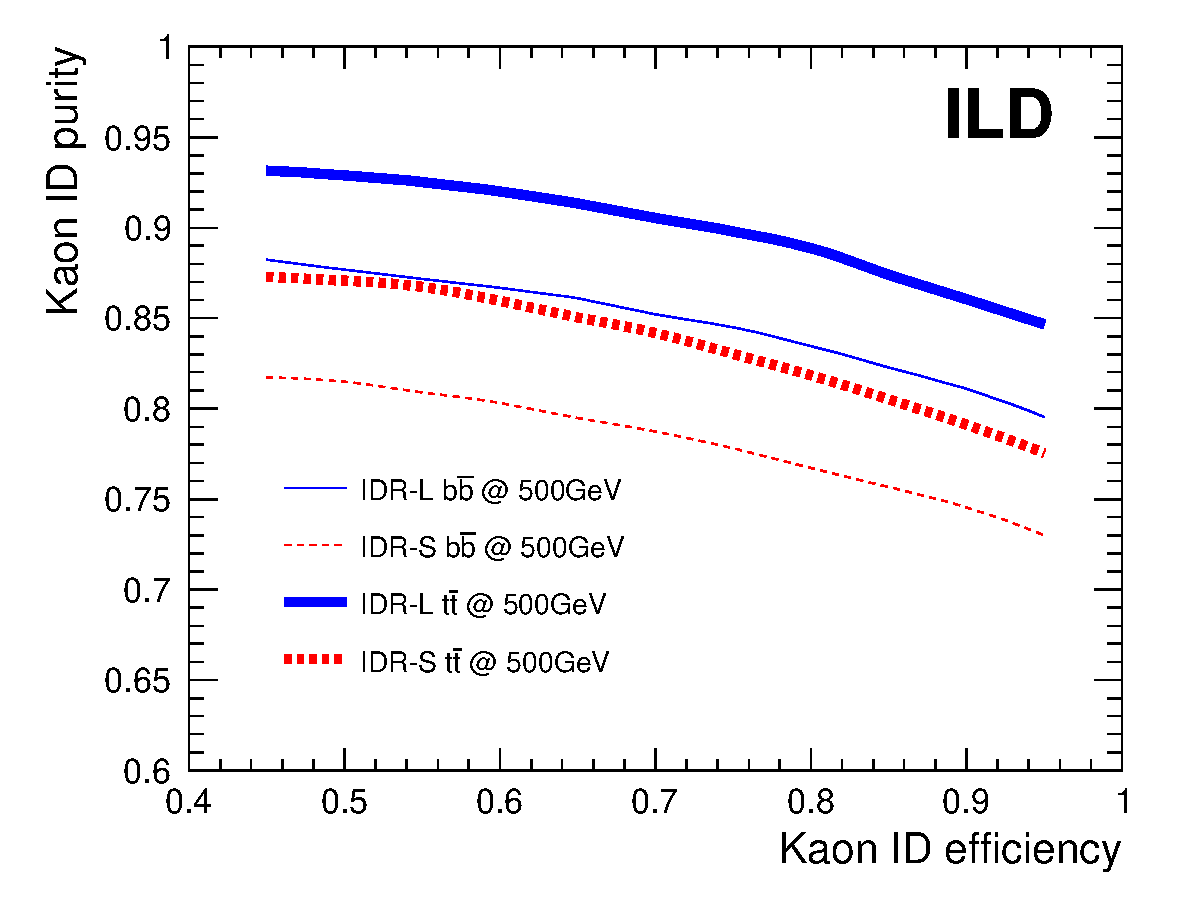
\includegraphics[width=0.8\hsize]{Performance/fig/kaonIDeff_v2-eps-converted-to.pdf}
  \caption{\label{fig:perf:KaonID}
    Efficiency-purity curves for charged Kaon identification in the context of the $t\bar{t}$ and $b\bar{b}$ analyses. For the same
    efficiency, the large detector reaches a $5\%$ higher purity due to its larger number of TPC measurements, which results in a better $dE/dx$
    resolution. Details on the analyses can be found in Sec.~\ref{subsec:bench:bbbar} and~\ref{subsec:bench:ttbar}.
  }
\end{figure}
Additional methods for charged particle identification using calorimeter shower shapes have also been developed and used in specific physics analyses.
%~\fix{[need references...]}


%%%%%%%%%%%%%%%%%%%%%%%%%%%%%%%%%%%%%%%%%%%%%%%%%%%%%%%%%%%%%%%
\subsection{BeamCal reconstruction}

Many analyses require the efficient measurement of electromagnetic showers at small polar angles in the BeamCal.
Due to the large amounts of background from pair particles (c.f.~\ref{sec:beam:background}), the BeamCal requires a special reconstruction algorithm
for identifying showers in the presence of background.
Fig.~\ref{fig:perf:beamcal_eff} shows the achieved reconstruction efficiency for single \unit{30}{\GeV} photons for the large and small detector models
for $E_{cms}=\unit{500}{\GeV}$  and $E_{cms}=\unit{250}{\GeV}$ respectively. Due to the significantly larger backgrounds at \unit{500}{\GeV} the efficiency
rises slower with polar angle than at \unit{250}{\GeV} and there is almost no difference observed between the two models.
In contrast at lower center of mass energy the small detector shows better performance, as expected due to the reduced background as an effect of the
higher B-field. Here a plateau of the efficiency at $\approx 80\%$~is reached between \unit{15}{\mrad} and \unit{20}{\mrad} due to the keyhole opening
of the BeamCal front face.
Fig.~\ref{fig:perf:beamcal_fake} shows the fraction of events where ... \fix{need updated plot and proper definition of what is plotted here ...}
%
% BeamCal Reco for single electrons
%
\begin{figure}[htbp]
\begin{subfigure}{0.49\hsize}
 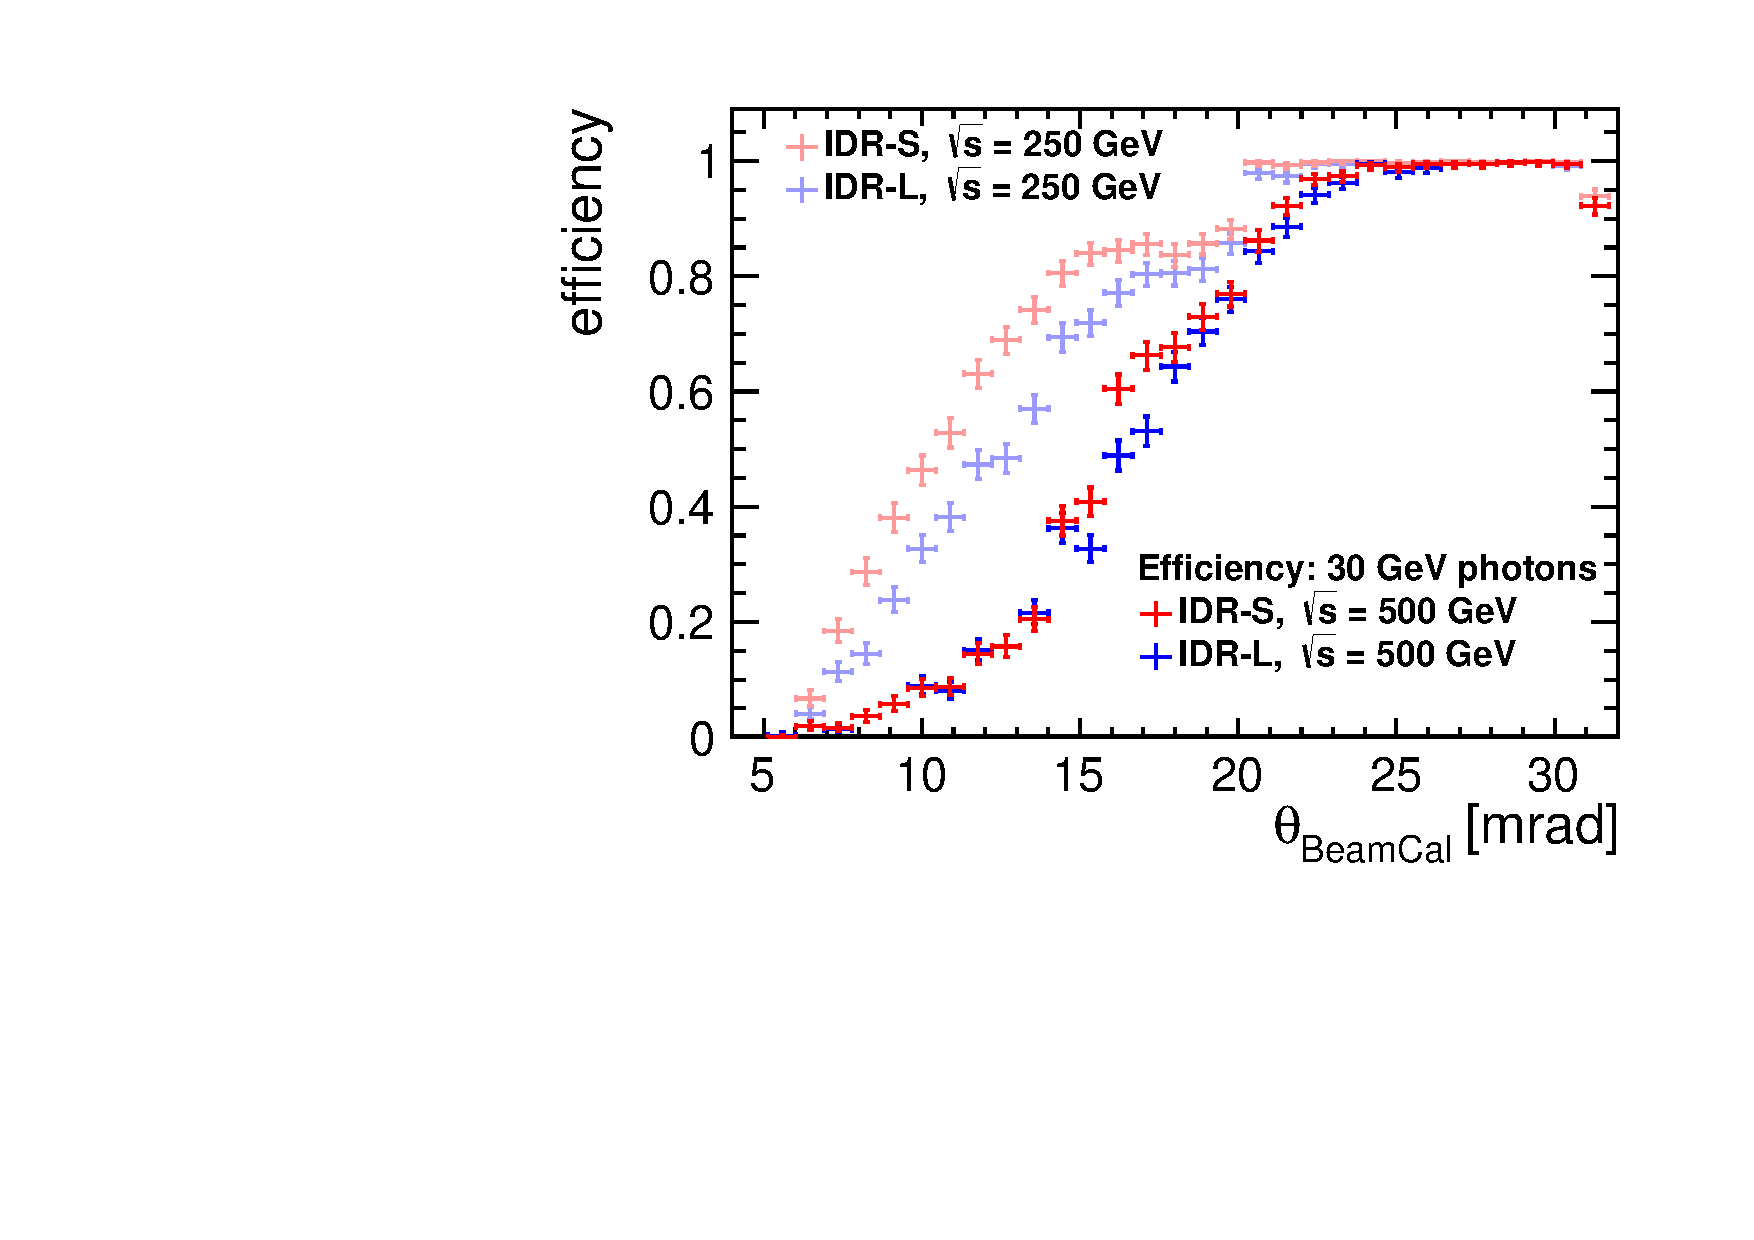
\includegraphics[width=\hsize]{Performance/fig/Eff_30GeVPhotons_different_detectors_differentCOMenergies.pdf}
 \caption{ \label{fig:perf:beamcal_eff}}
 \end{subfigure}
\begin{subfigure}{0.49\hsize}
 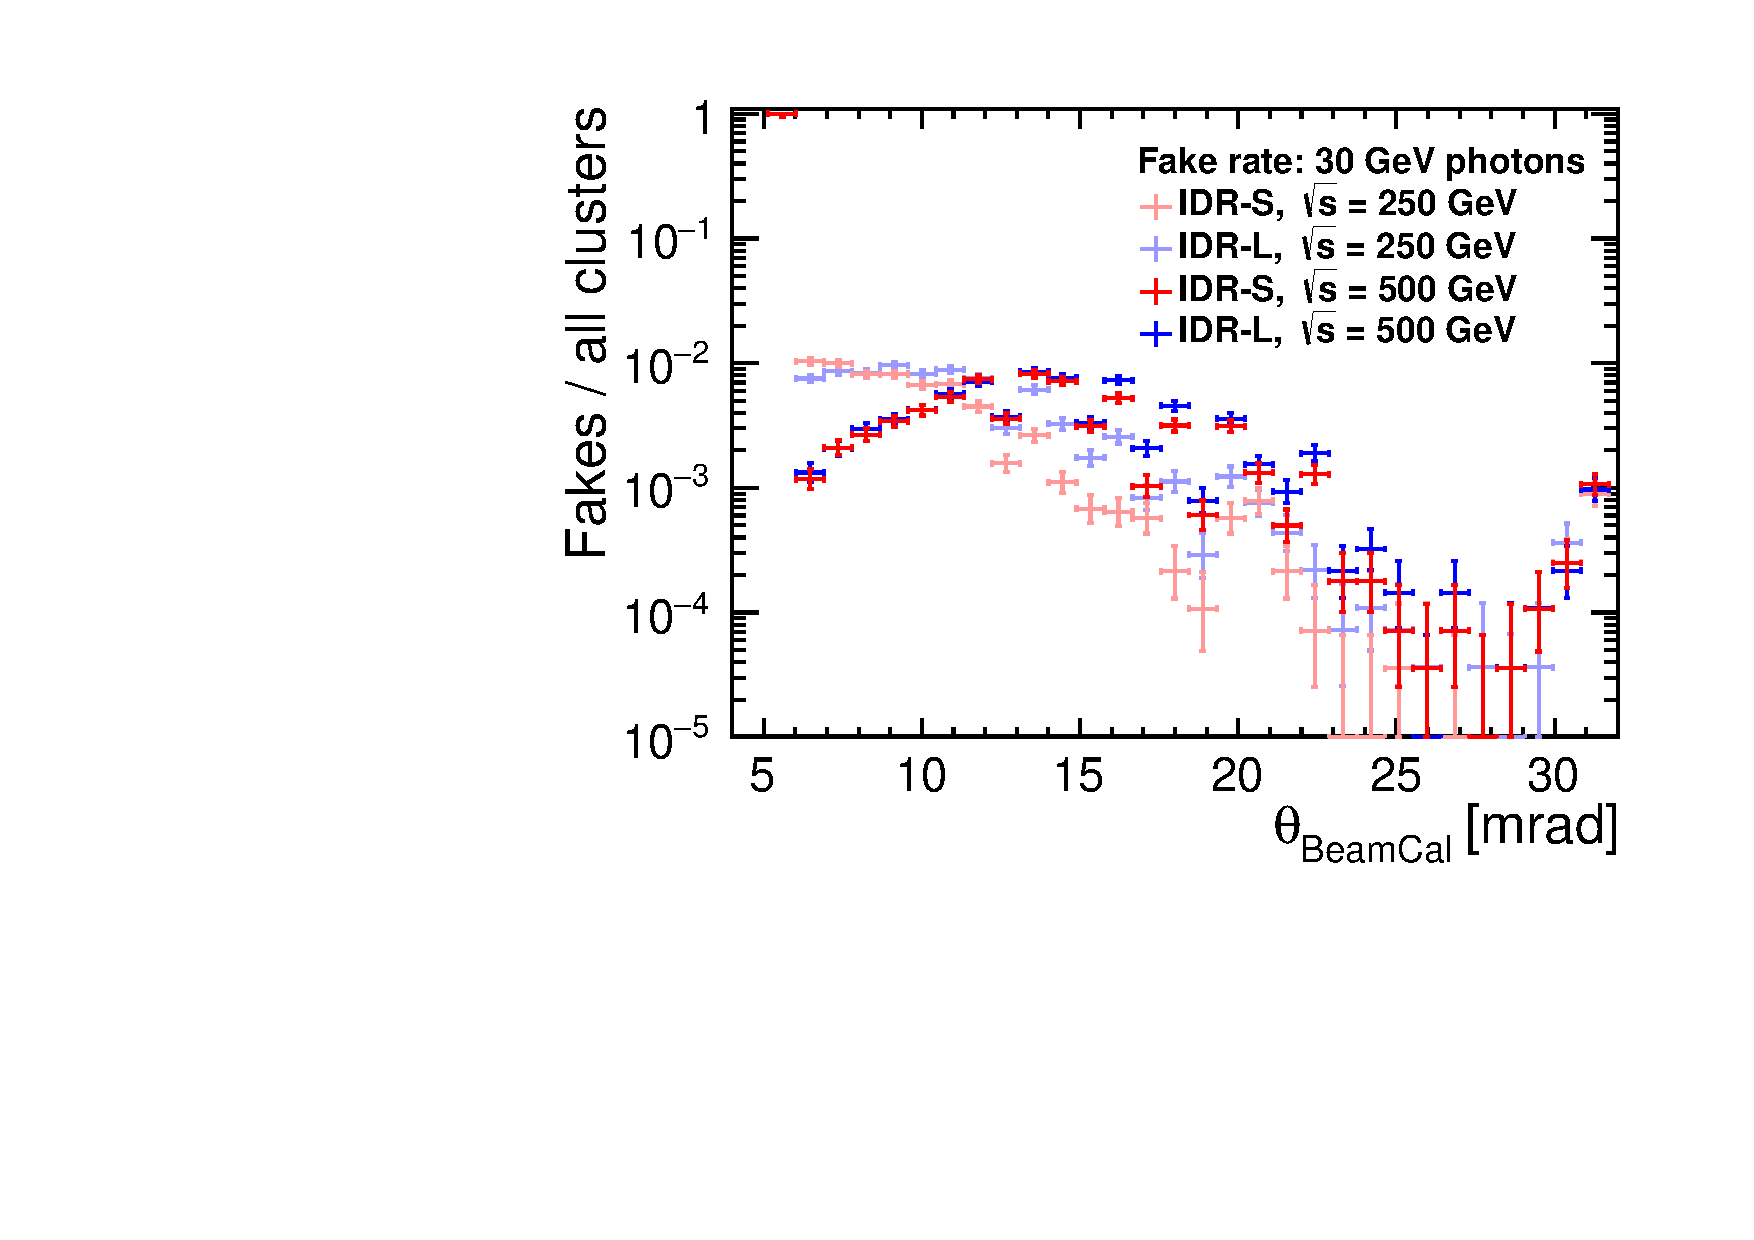
\includegraphics[width=\hsize]{Performance/fig/Fakes_30GeVPhotons_different_detectors_differentCOMenergies.pdf}
 \caption{  \label{fig:perf:beamcal_fake}}
 \end{subfigure}
\caption{ (a) Reconstruction efficiency for single \unit{30}{\GeV} photons in the large and small detector models for $E_{cms}=\unit{500}{\GeV}$  and
  $E_{cms}=\unit{250}{\GeV}$.
  (b)  Fake rate ...  1-purity ... \fix{need updated plot and proper definition of what is plotted here ...}
}
\label{fig:perf:beamcal}
\end{figure}



%%%%%%%%%%%%%%%%%%%%%%%%%%%%%%%%%%%%%%%%%%%%%%%%%%%%%%%%%%%%%%%%%%%%%%%%%%%%%%%%

\section{\label{sec:HLR-performance} High-level Reconstruction Performance}
\writer{Frank Gaede, Jenny List}{5}

\subsection{Flavour-Tag Performance}
\label{sec:perf:hlr:lcfi}
The efficient identification of heavy flavour jets in hadronic events is an indispensable ingredient to many important physics analyses, such as
the $\PH\rightarrow\Pqc\APqc$ and $\PH\rightarrow\Pqb\APqb$ branching ratio  measurements.
The flavour tagging performance is studied using simulated and fully reconstructed samples
of dedicated $\Pep \Pem \rightarrow 6~\Pquark$ events at $\sqrt{s}=\unit{500}{\GeV}$, where all quarks are chosen to have the same flavour.
The samples are divided into two sub-samples, where one is used for training the BDT and the other is used
as a test sample. The resulting performance is shown in Fig.~\ref{fig:HLR-flavtag} for the large and small ILD detector model.
In (a) the background rate as a function of the c-tagging efficiency for b-quark and light flavour quark jets is plotted and (b) shows the
 background rate for c-quark and light flavour quark jets as a function of the b-tagging efficiency.
%
\begin{figure}[htbp]
\begin{subfigure}{0.49\hsize}
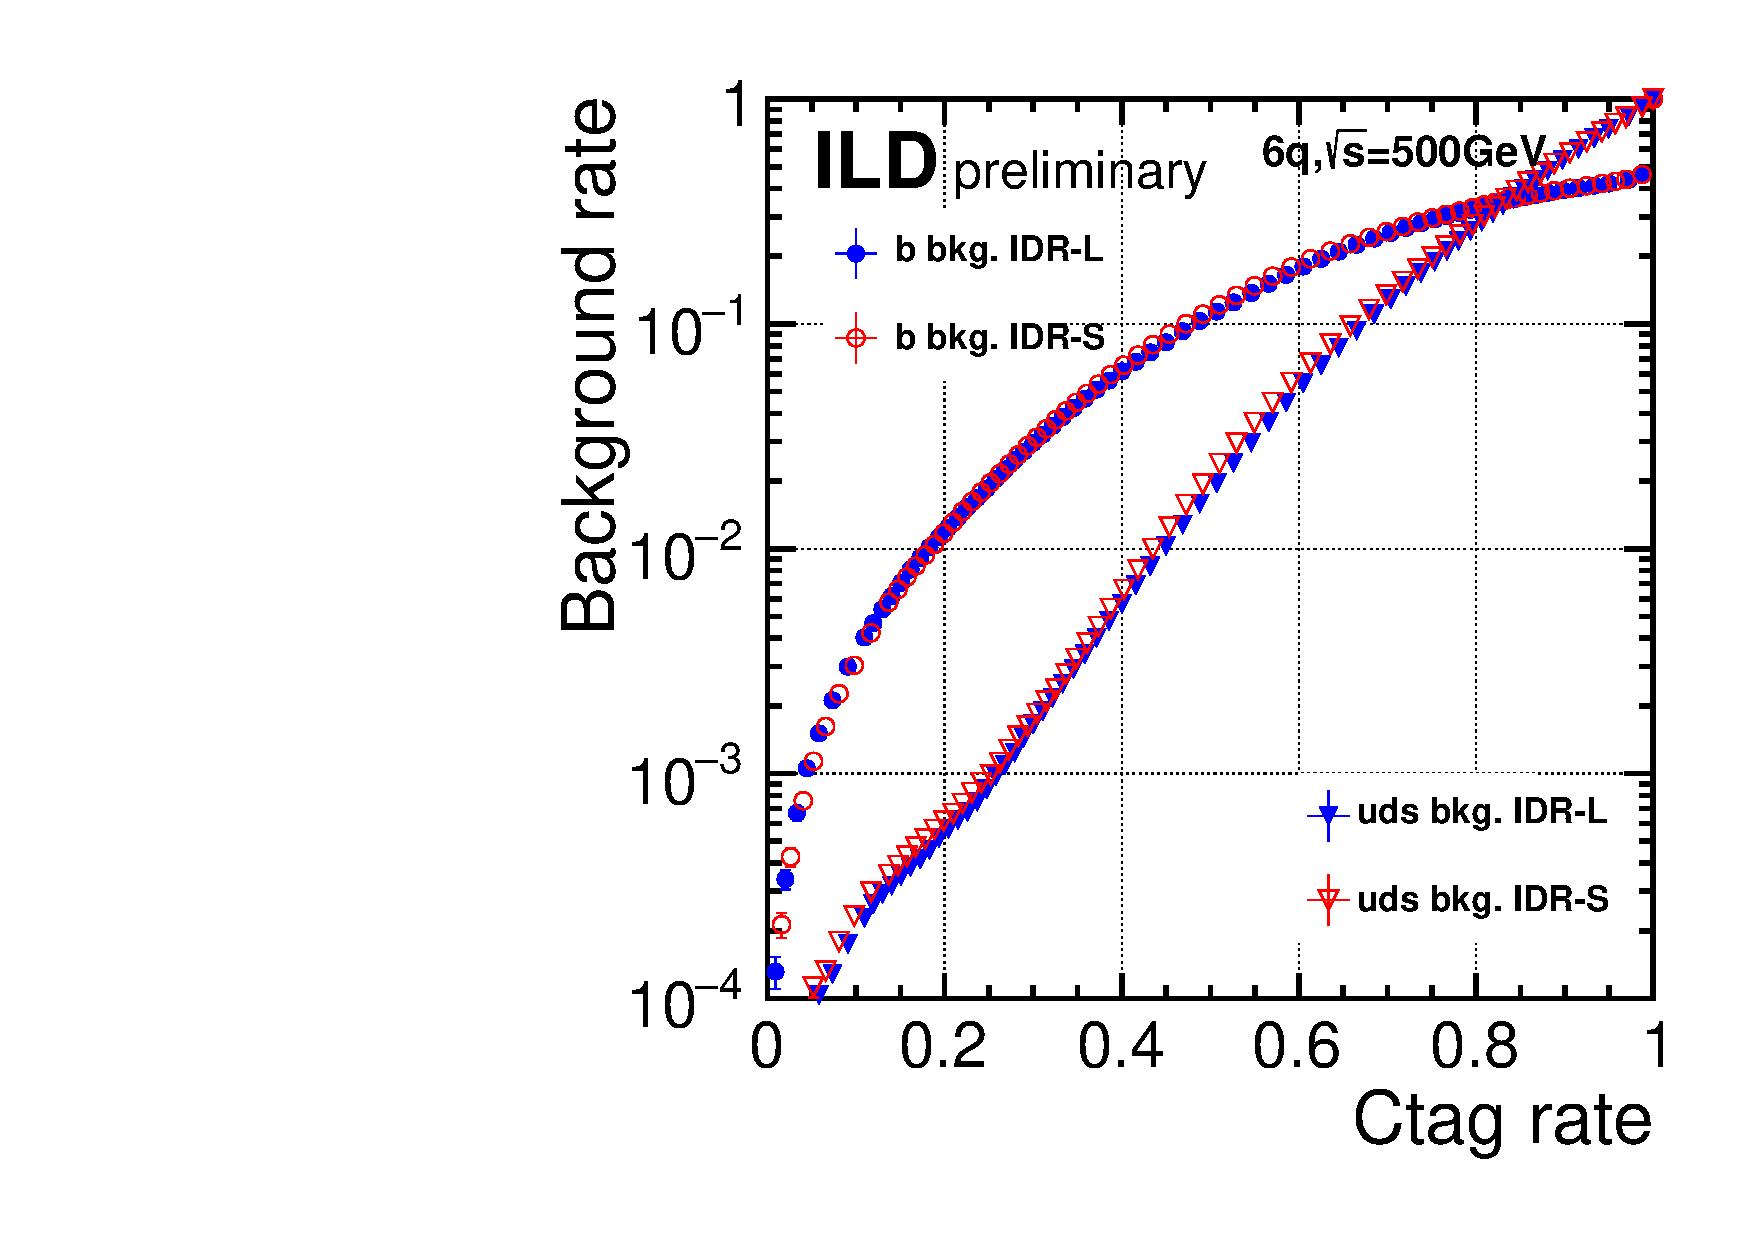
\includegraphics[width=\textwidth]{Performance/fig/ctag_performance.pdf}
 \caption{ \label{fig:HLR-ctag_perf}}
 \end{subfigure}
\begin{subfigure}{0.49\hsize}
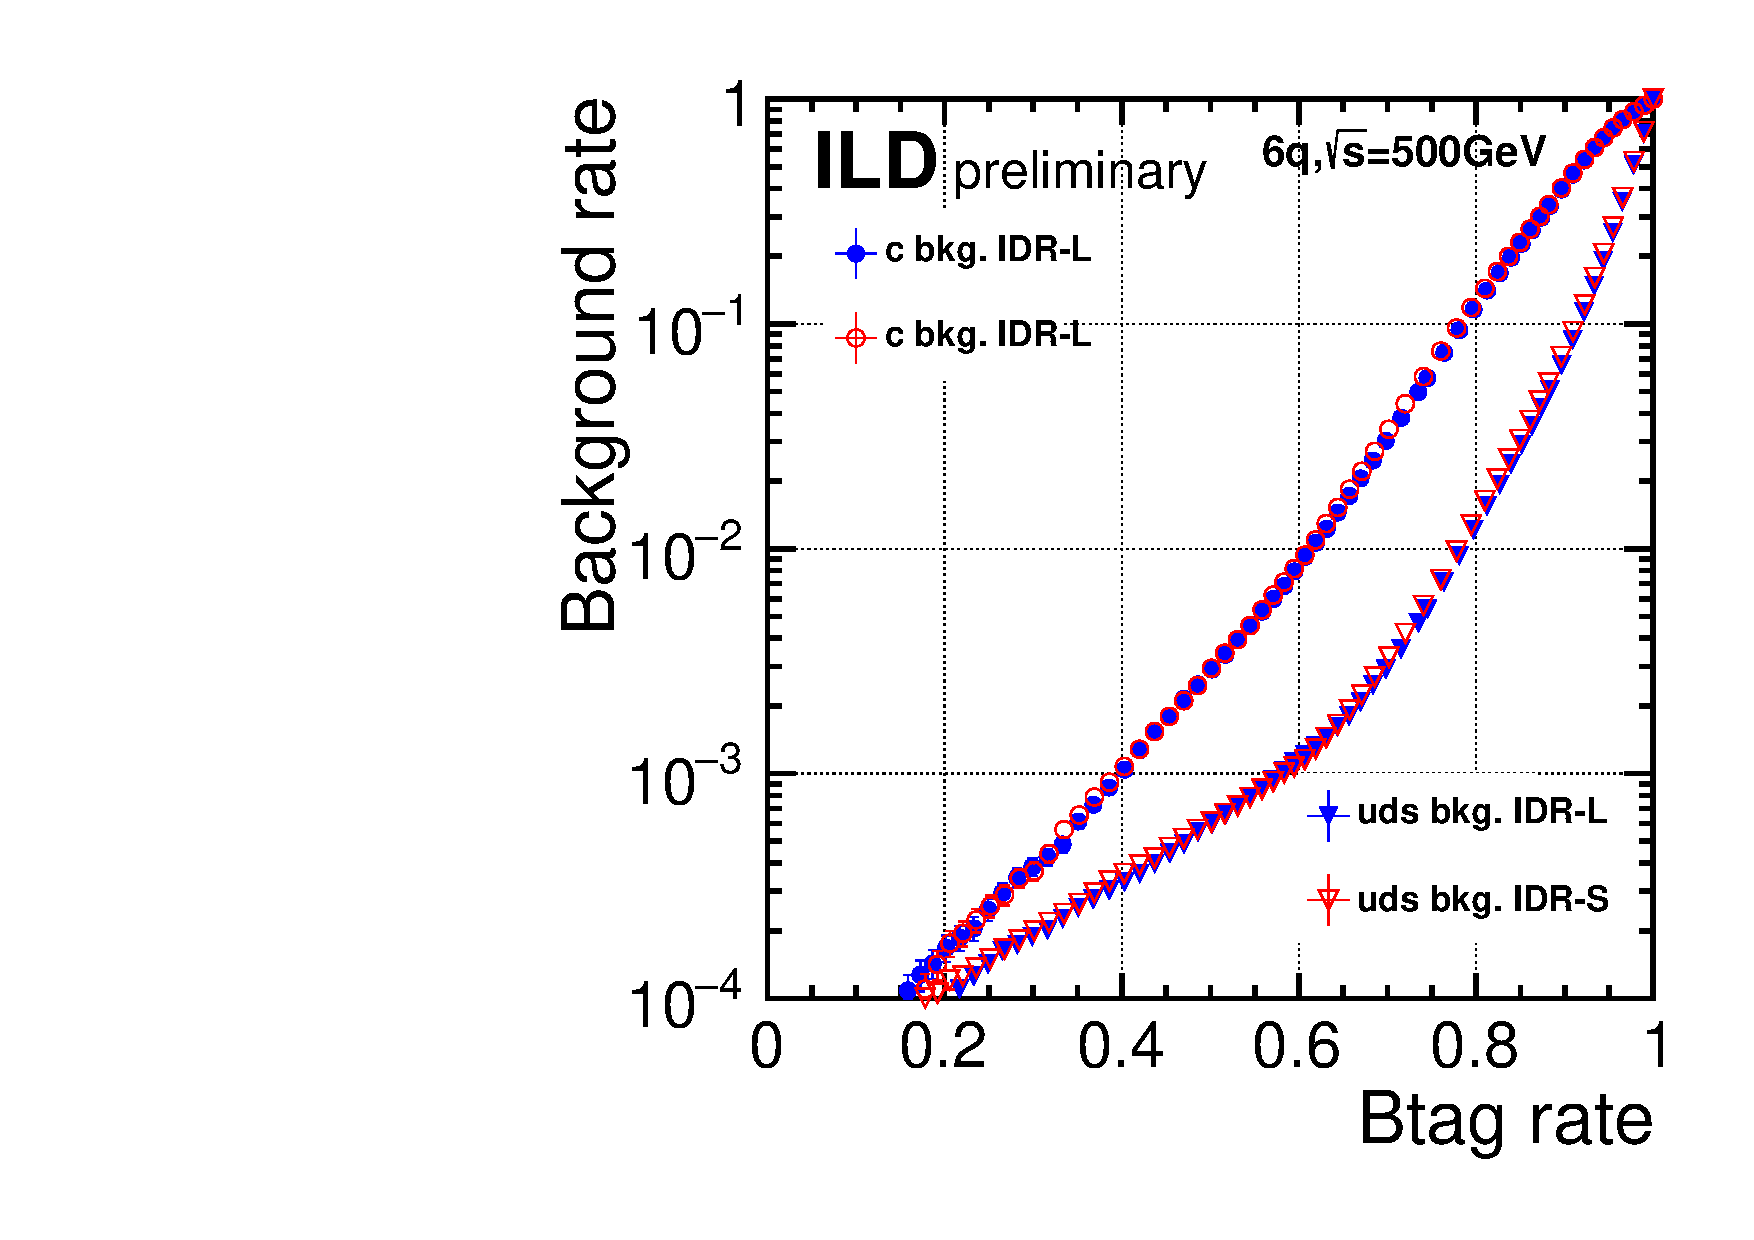
\includegraphics[width=\textwidth]{Performance/fig/btag_performance.pdf}
 \caption{  \label{fig:HLR-btag_perf}}
 \end{subfigure}
\caption{Flavour tag performance for the large and small ILD detector models. (a) background rate as a function of the c-tagging efficiency
  for b-quark and light flavour quark jets. (b) background rate as a function of the b-tagging efficiency for c-quark and light flavour quark jets. }
\label{fig:HLR-flavtag}
\end{figure}
%
As expected from the impact parameter and vertex resolutions there are no significant differences observed between the large and small ILD variants
for the flavour tagging performance.
The flavour tagging performance has been seen to vary with the jet energy and jet multiplicity~\cite{Suehara:2015ura}.
The ideal performance in a physics study can be achieved by retraining the BDTs for the corresponding signal event topology.
In practice, several sets of training weights are centrally produced, which are compared and chosen for the best performance.

%\subsection{neutral - \Ppizero}
\subsection{Hadronically decaying $\tau$ ID}
\label{sec:perf:hlr:tau}

The correct identification of $\tau$ lepton decay modes is of particular importance in the extraction of observables sensitive to the $\tau$ lepton spin direction: examples are measurements of the $\tau$ polarisation and Higgs CP based on spin correlations in $H \to \tau \tau$ decays.
Hadronic $\tau$ decays are typically offer the most sensitivity to the spin, due the presence of a single neutrino. 
The identification of these hadronic decay modes can be factorised into the charged and neutral components. 
The charged part is typically rather straight-forward in the TPC of ILD, so we concentrate efforts on understanding the identification of the neutral part, which consists largely of photons from neutral pion (and to a lesser extent other neutral meson) decays. 
In the decays of highly boosted taus, these photons are typically rather close to both a charged particle and one or more additional photons produced in the same $\tau$ decay. 
The separation between these photons in the calorimeter depends on its inner radius, while the distance to charged particles additionally depends on the magnetic field strength. 
We can therefore expect some differences in performance for the large and small ILD detector models.

The performance of $\tau$ decay mode identification was studied in $\tau$-pair production events at a centre-of-mass energy of $500$\,GeV. 
These very highly boosted $\tau$ decays are the most challenging to reconstruct due to the small distance between particles in the highly collimated $\tau$ decay jets.
The standard ILD reconstruction algorithms were applied to these events.

In each event, two high momentum, back-to-back, charged PFOs were identified as $\tau$ jet "seeds". Figure~\ref{fig:HLR-tauID} shows the number of photon PFOs identified in a cone around these $\tau$ seed tracks, in the case when the $\tau$ lepton decayed to $\pi^\pm \pi^0 \nu$.
In these events, exactly two photons are expected in the vast majority of cases. 
The distribution shows that it is challenging to reconstruct both photons: in around half of the cases only a single photon cluster was reconstructed, which is due to the merging of the two photons into a single reconstructed particle. 
A difference is seen between the two detector models, with the large version somewhat more often correctly resolving the two photons, which can be understood as being due to the larger ECAL radius increasing the distance between the photons' electromagnetic showers.


\begin{figure}[htbp]
\begin{subfigure}{0.49\hsize} 
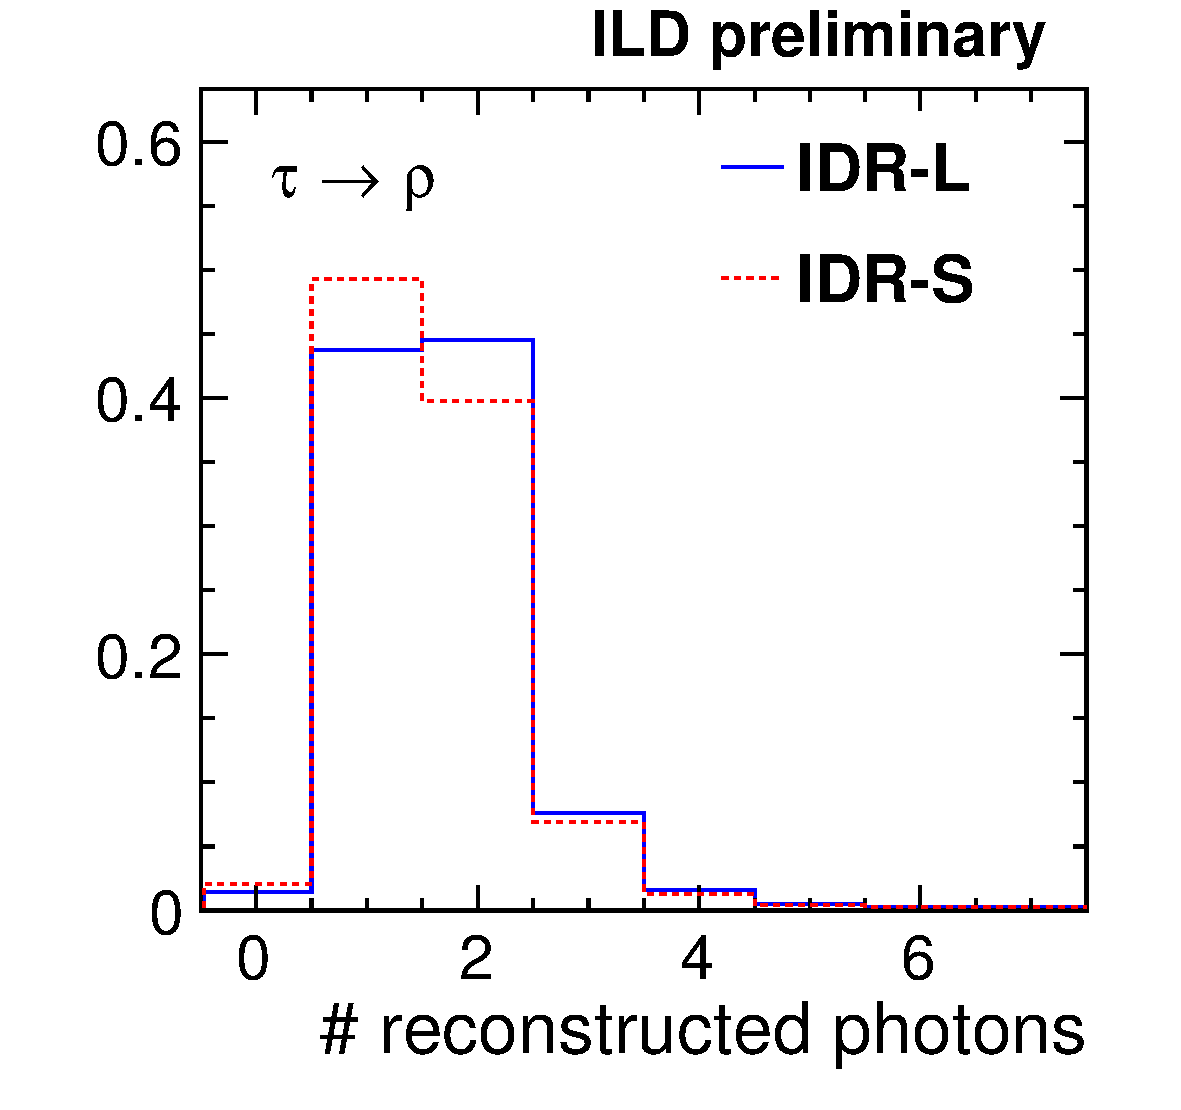
\includegraphics[width=\textwidth]{Performance/fig/tauID_ngammapfo.pdf}
 \caption{ \label{fig:HLR-tauID:ngamma}}
 \end{subfigure}
\begin{subfigure}{0.49\hsize} 
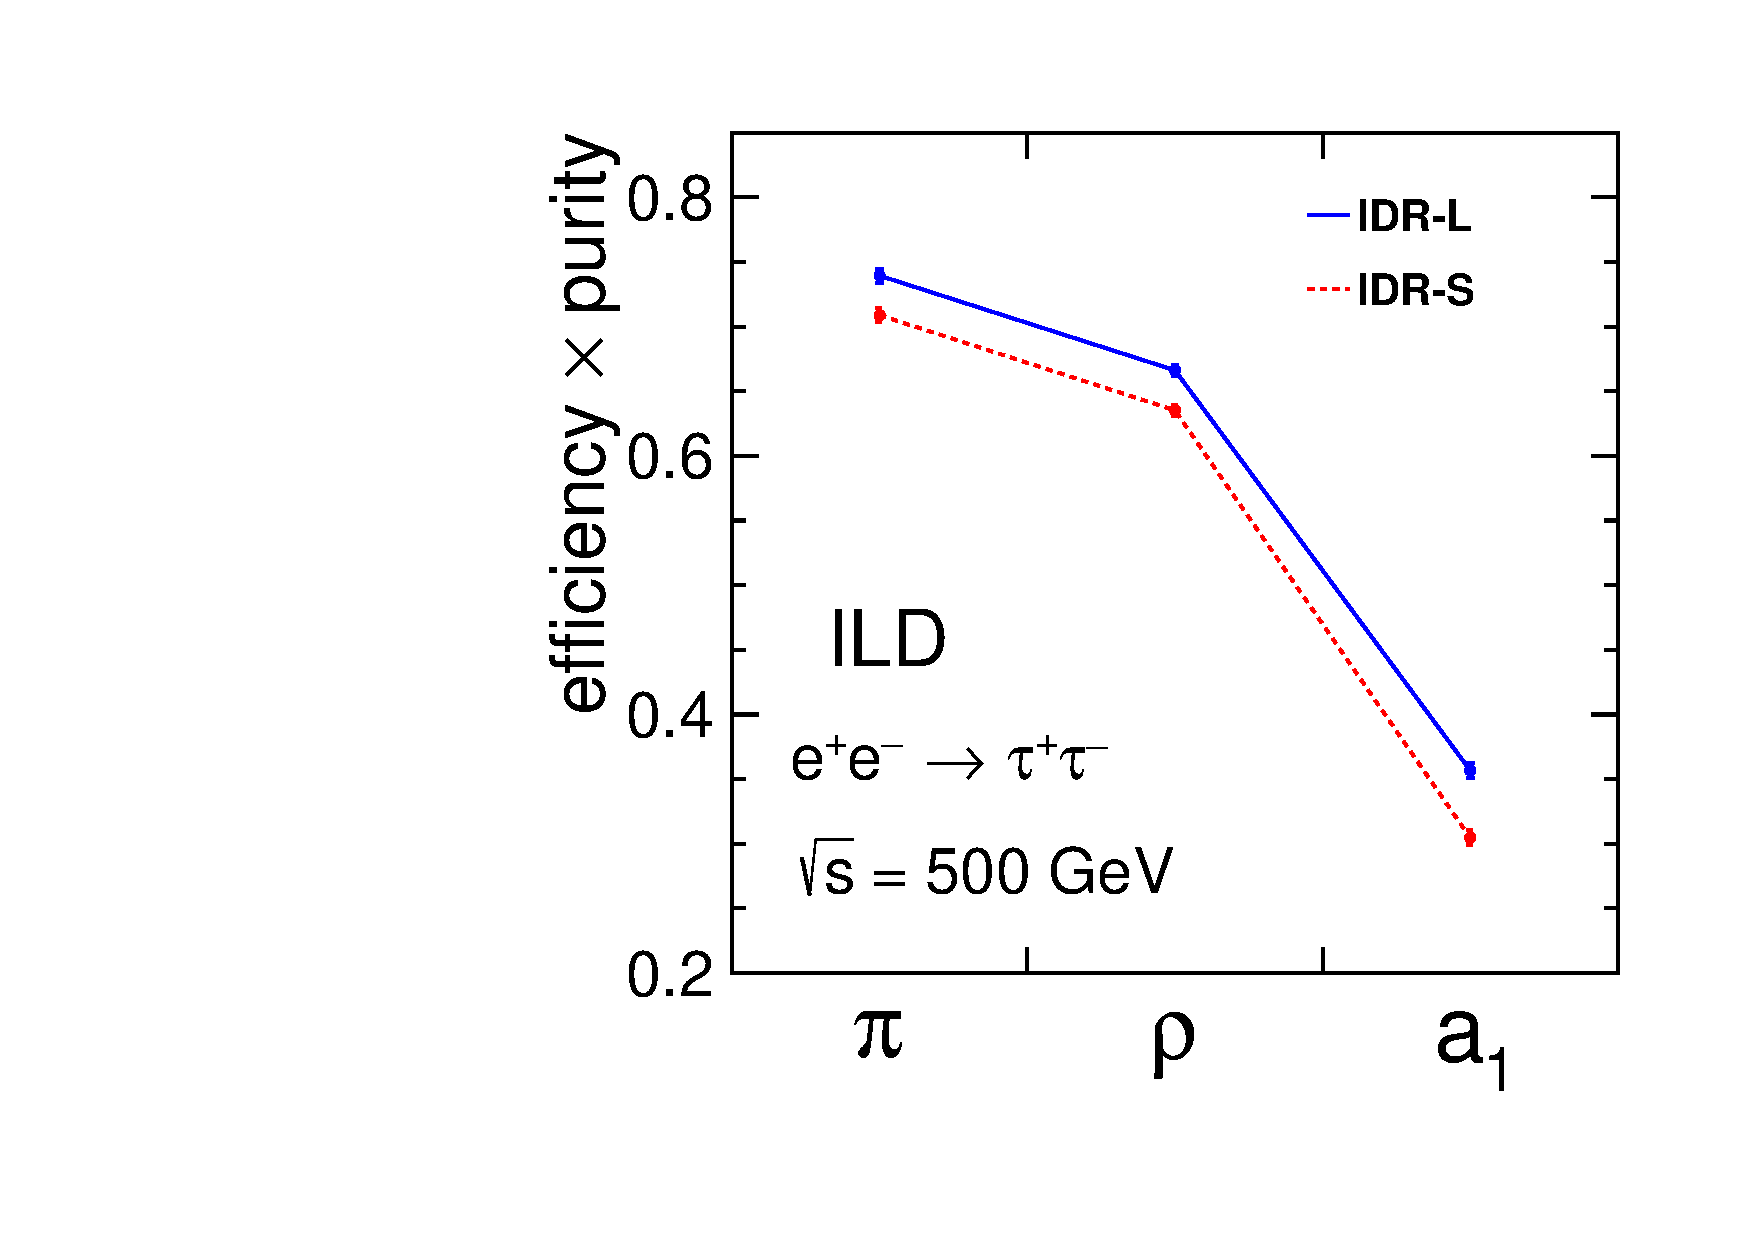
\includegraphics[width=\textwidth]{Performance/fig/tauID_effPur.pdf}
 \caption{  \label{fig:HLR-tauID:effpur}}
 \end{subfigure}
\caption{Hadronic decay mode identification for isolated $\tau$-leptons with momenta near $250$\,GeV.
(a) The number of reconstructed photon PFOs in  $\tau \to \rho \nu \to \pi^\pm \pi^0 \nu$.
(b) The performance of a simple $\tau$ decay mode identification algorithm.
}
\label{fig:HLR-tauID}
\end{figure}


A simple cut-based approach to the identification of single-prong hadronic $\tau$ decays was developed, based on the number of reconstructed photon PFOs, and the invariant mass of this set of photon PFOs both alone and together with the charged PFO around which the $\tau$ candidate jet was built.
The ability of this algorithm to distinguish $\tau \rightarrow \pi^\pm \nu$ ("$\pi$"), $\tau \rightarrow \pi^\pm \pi^0 \nu$ ("$\rho$"), and $\tau \rightarrow \pi^\pm \pi^0 \pi^0 \nu$ ("$\mathrm{a_1}$") decays is shown in Fig.~\ref{fig:HLR-tauID}. 
The product of selection efficiency and purity varies between around 30\% and 75\% among these three decay modes.
The large detector model performs slightly better, as expected thanks to the larger inner ECAL radius.

%\subsection{V0 / in flight decays vs radius}
\subsection{$J/\psi$ reconstruction}
With the excellent particle flow, particle identification and vertexing capabilities
of ILD discussed in the previous sections, there is a great potential to reconstruct
various exclusive decay chains of short-lived baryons and mesons. This is of special
interest in case the ILC will be operated at the $Z$ pole, but also at higher energies we expect further improvements to flavour tagging and jet energy resolution
once this potential is fully exploited in reconstruction and analyses. This is an area where new algorithmic developments could still lead to a significant improvement
of the ILD performance.

At the current stage, we only provide a very simple example, namely the reconstruction of $J/\psi \to \mu^+\mu^-$ decays. Due to its extremely well-known mass (known to 3.6\,ppm~\cite{Tanabashi:2018oca}), the $J/\psi$ is an important standard candle, e.g.\ for calibration of the tracker momentum scale.

\begin{figure}[htbp]
\begin{center}
 \includegraphics[width=0.75\textwidth]{Performance/fig/Jpsi_InvMassS5_vs_L5.pdf}
\end{center}
\caption{$J/\psi \to \mu^+\mu^-$ candidates as reconstructed with IDR-L and IDR-S.}
\label{fig:hlr:jpsi}
\end{figure}

Figure~\ref{fig:hlr:jpsi} shows the invariant mass spectrum of reconstructed muon pairs in the $J/\psi$ region, comparing the large and small detector. All available
SM MC events from the optimisation production at $\sqrt{s}=500$\,GeV have been used and weighted to the full luminosity of $4$\,ab$^{-1}$ with the canonical sharing between the polarisation configurations. The combinatorial background has been determined from like-sign muon pairs and has been subtracted from the opposite-sign pairs, leading to the fluctuations around zero in the off-peak regions.
At $500$\,GeV, most $J/\psi$ candidates are produced in the forward direction, with $|\cos{\theta}|>0.8$ and at rather low transverse momenta, typically below $30$\,GeV.
Therefore, the small detector has a smaller acceptance than the large detector, with about $10$k vs $12$k recontructed $J/\psi$'s compared to about $20$k available at generator level. On the other hand, the better momentum resolution of the small detector in the forward region leads to a more narrow peak.
% \fix{
% \begin{itemize}
% \item $\Lambda^+_c \to pK^- \pi^+$
% \item $D^0$, $D^*$
% \item $J\psi \to \mu \mu$  / inclusive di-muon spectrum ?
% \end{itemize}
% }

% \subsection{Di-jet mass resolution between Cambridge and full physics}
% \begin{itemize}
% \item $Z$ mass in $ZZ \to \nu\nu qq$, flavour separated
% \item $W$ hadronic mass from $WW \to qq l\nu$
% \item from Jakob $\nu\nu qqqq$
% \item various levels of cheating with TrueJet
% \end{itemize}



%%%%%%%%%%%%%%%%%%%%%%%%%%%%%%%%%%%%%%%%%%%%%%%%%%%%%%%%%%%%%%%%%%%%%%%%%%%%%%%%

\section{\label{sec:benchmarks} Physics Benchmarks}
\writer{Jenny List}{20}

%\subsection{General Remarks}
\fix{Each benchmark has its own confluence page, where a lot more material, including the draft of the ILD note and the names of the main analysis reponsibles can be found: {\small \url{https://confluence.desy.de/display/ILD/Benchmarks+for+physics-driven+detector+optimisation}} 
Note that several benchmark are still work in progress. A short comment at the beginning of each section gives a rough summary of the status.}

The performance of the two ILD detector models IDR-L and IDR-S has been
evaluated on a number of physics benchmarks, which will be discussed in this section. Despite the fact that a 250-GeV version of the ILC is currently under political consideration in Japan, the detector benchmarking has been performed at higher center-of-mass energies, mostly at 500\,GeV, and in one case even at 1\,TeV. This choice has been made in order to make sure that both detector models perform adequately also under the more challenging experimental conditions of the higher energy stages, and in order to cover e.g.\ a wider range of jet, lepton and photon energies.

Unless stated otherwise, all results have been scaled to the integrated luminosity and beam polarisation of the full H20 running scenario originally defined in~\cite{Barklow:2015tja}, which is --- for the higher center-of-mass energies --- unchanged since~\cite{Bambade:2019fyw}. In particular, the H20 scenario comprises 4\,ab$^{-1}$ at 500\,GeV, with beam polarisation absolute values of 80\% for the electron and 30\% for the positron beam. The total luminosity is shared between the different polarisation sign combinations according to $f(-+,+-,++,--) = (40\%,40\%, 10\%, 10\%)$. 
Analoguously, 8\,ab$^{-1}$ are considered at 1\,TeV, with absolute polarisation values of 80\% for the electron and 30\% for the positron beam, with the same $f(-+,+-,++,--) = (40\%,40\%, 10\%, 10\%)$ sharing.

The benchmarks presented in this section have been chosen to illustrate many performance aspects with a minimum number of physics channels, and are not to meant to cover the {\em complete} physics case. The main focus of the analysis work was not always the pure optimisation for utmost physics performance, but rather to better understand and highlight the role of individual performance aspects and their interplay.

Unless stated otherwise, the analyses performed for and since the time of the DBD remain valid in their physics message. For an up-to-date review of the ILC physics case, based on ILD detector simulations, see e.g.~\cite{Bambade:2019fyw}.

%%%%%%%%%%%%%%%%%%%%%%%%%%%%%%%%%%%%%%%%%%%%%%%%%%%%%%%%%%%%%%%%%%%
\subsection{Hadronic Branching Ratios of the Higgs Boson}
\fix{few open questions between Masakazu, Frank Simon and JL, see email June 25.}

The measurement of the hadronic branching ratios of the Higgs boson,
including in particular $H\to c\bar{c}$, is one of the unique items
on the menu of future $e^+e^-$ colliders. This crucially depends on 
an excellent flavour tag, c.f.\ Sec.~\ref{sec:perf:hlr:lcfi}, enabled
by vertex detectors with micrometer point resolution with a first layer placed as close as 1.6\,cm to the beam line.

As a benchmark, the $\nu \bar{\nu} H \to \nu \bar{\nu} jj$ final state was chosen in order to minimize the impact of other performance aspects like e.g.\ jet clustering. Thus the target physics observable here is $\sigma(\nu\bar{\nu} H)\times BR(H\to b\bar{b} / c\bar{c} / gg)$. With the full 500\,GeV data set, about 200000 $H \to b\bar{b}$ events would be produced in this final state alone, while about 30000 and 10000 $H \to gg$ and $H \to c\bar{c}$ would be available, respectively. In the 
limit of 100\% signal efficiency and zero background, this would correspond to statistical precisions of 0.2\%, 0.6\% and 1\% for $H \to b\bar{b}$, $H \to gg$ and $H \to c\bar{c}$, respectively.

The benchmark analysis is documented in detail in~\cite{ILDNote:Hbbccgg}, and follows earlier analyses~\cite{Mueller:2016exq,Ono:2013voc,Ono:2013sea}. The full performance of the ILC on Higgs branching ratio measurements, combining all final states,  can be found in~\cite{Bambade:2019fyw}. After a cut-based preselection, the kinematic selection of $\nu \bar{\nu} H \to \nu \bar{\nu} jj$ events is refined by a multi-variate approach. Up to this point, no flavour-tag information is used.
Figure~\ref{fig:Hbbccgg:mh} shows the distributions of the reconstructed Higgs mass at this stage of the analysis for the signal on top of the remaining SM backgrounds, comparing both detector models.

\begin{figure}[htbp]
\begin{center}
 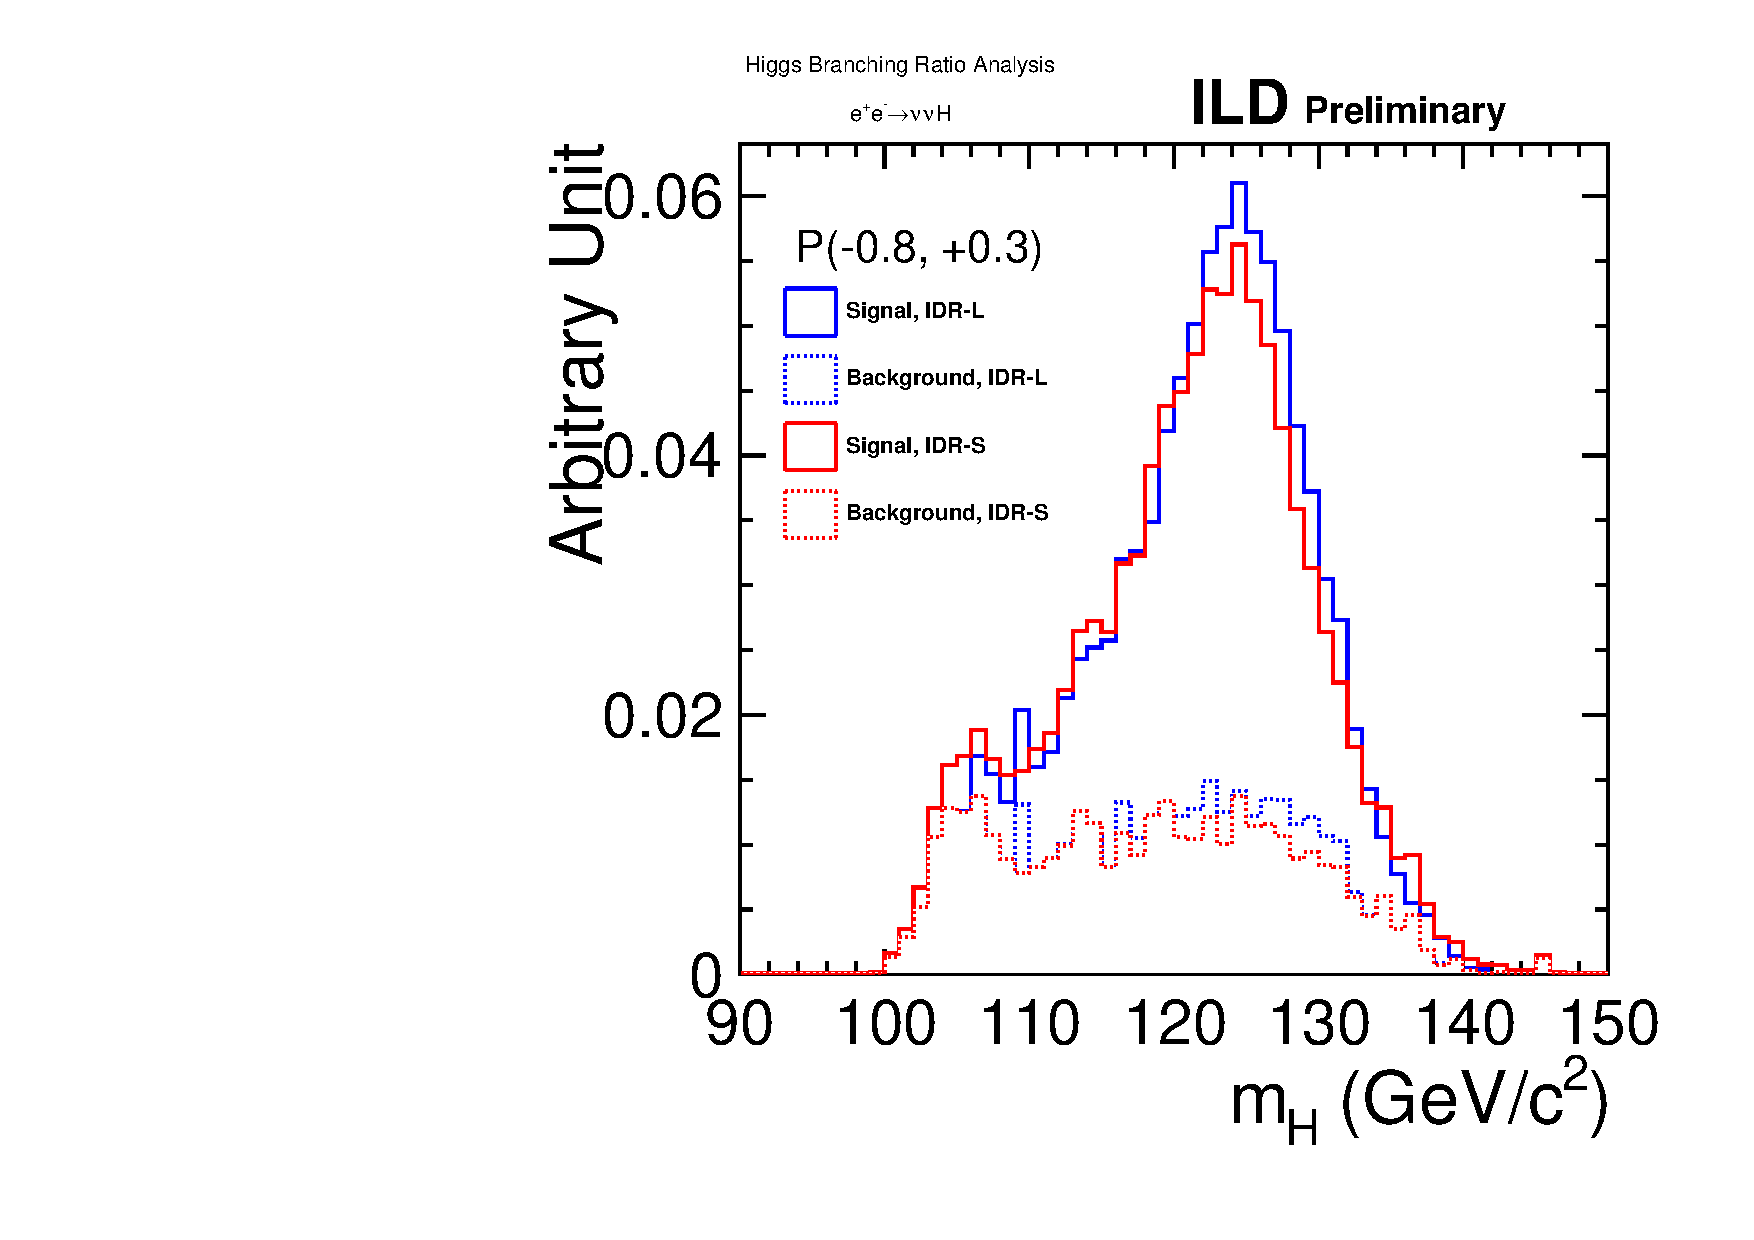
\includegraphics[width=0.5\textwidth]{Performance/fig/IDRplot5.pdf}
\end{center}
\caption{Reconstructed Higgs mass distribution after the kinematic selection. The signal is shown on top of the remaining SM background for both detector models.
}
\label{fig:Hbbccgg:mh}
\end{figure}


\begin{figure}[htbp]
\begin{center}
 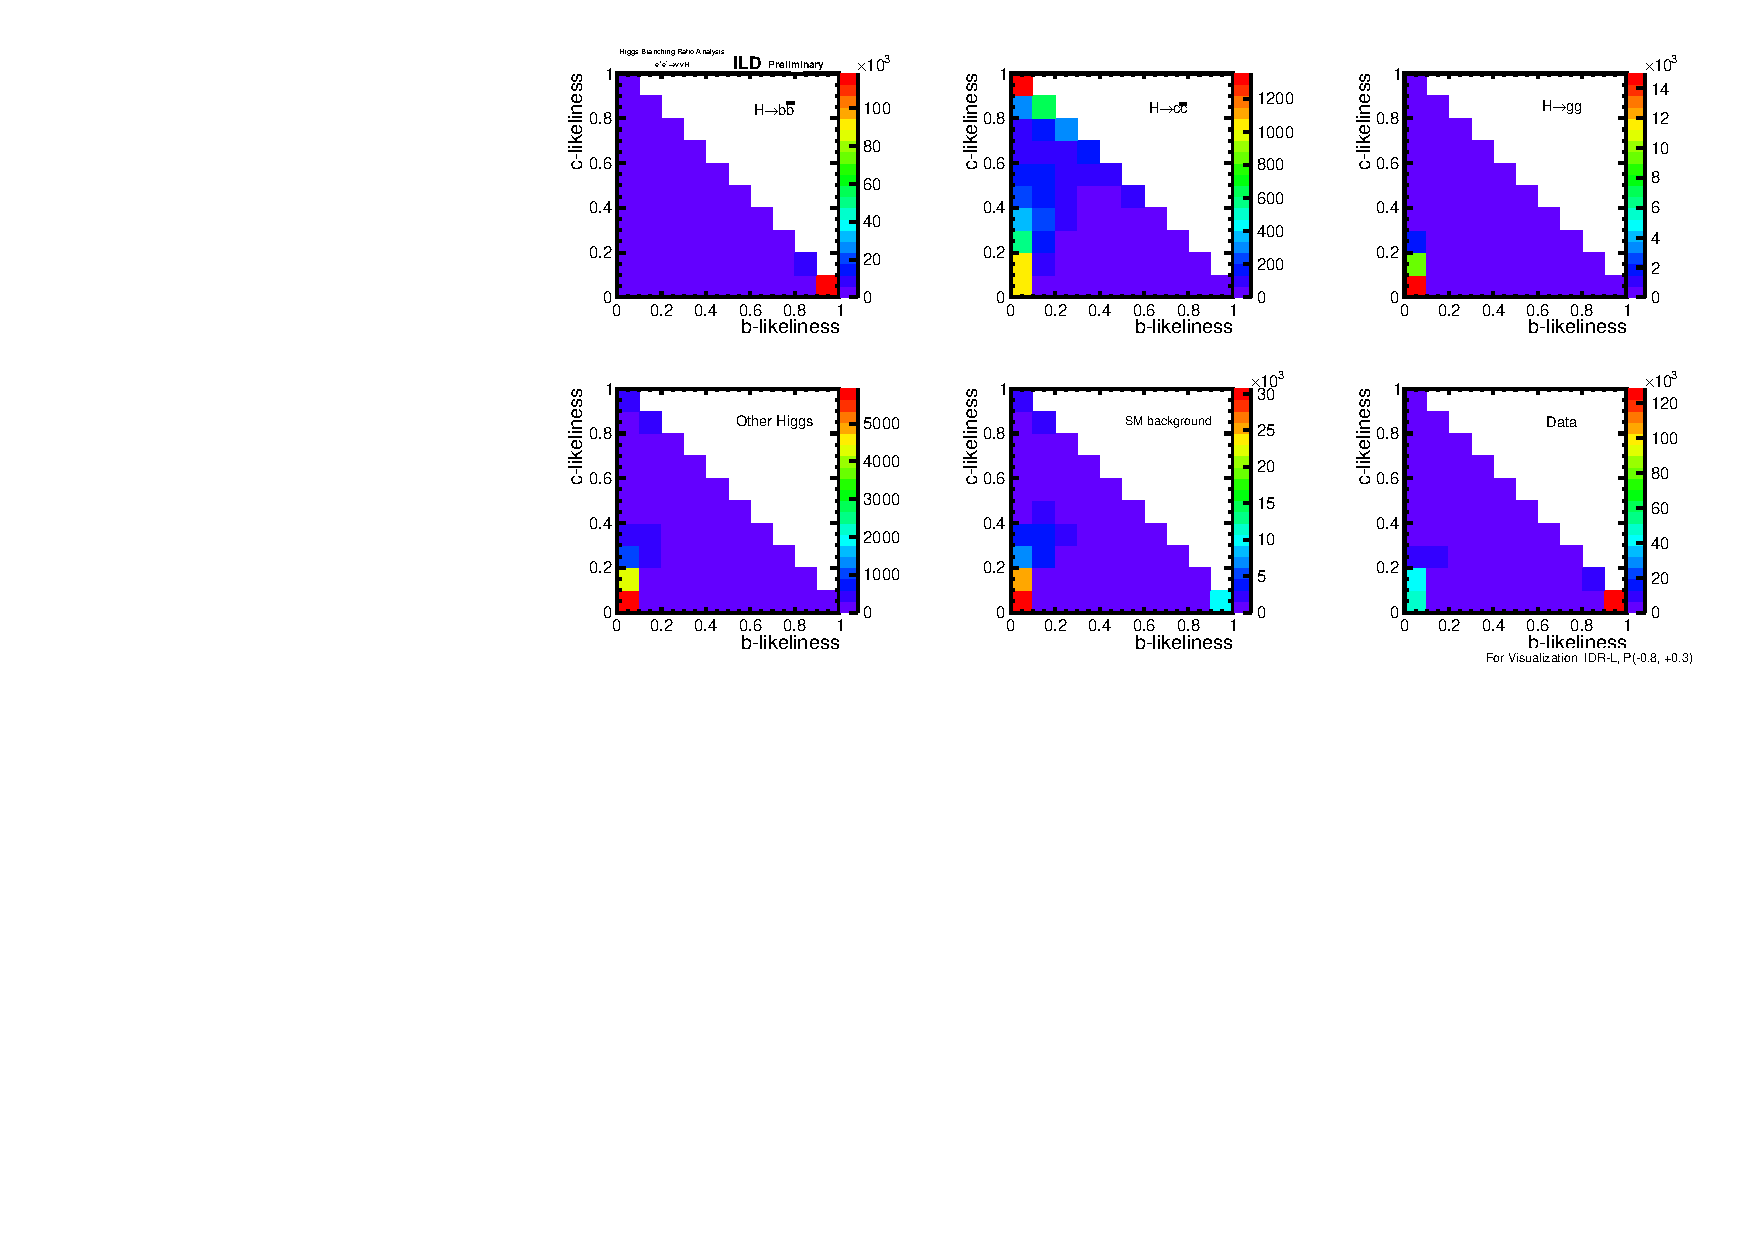
\includegraphics[width=\textwidth]{Performance/fig/IDRplot4.pdf}
\end{center}
\caption{Visulisation of the flavour tag performance in $\nu\bar{\nu} H$. The panels show the 2D distributions of $c$- vs $b$-likeliness separately for $H \to b\bar{b}$, $H \to c\bar{c}$, $H \to gg$, $H \to$other, the SM background and their mix expected in data.
}
\label{fig:Hbbccgg:likeli}
\end{figure}

Figure~\ref{fig:Hbbccgg:likeli} shows the 2D distributions of $c$- vs $b$-likeliness (c.f.\ Sec.~\ref{sec:perf:hlr:lcfi})for the different Higgs decay modes. The ``data'' distribution is then fitted in 3D template approach in order to determine the contained fractions of the various hadronic Higgs decay modes, where the 3rd dimension is the $bc$-likeliness. Due to the limited available statistics of background MC, a much smaller number of bins than displayed in Fig.~\ref{fig:Hbbccgg:likeli} was used~\cite{ILDNote:Hbbccgg}. The resulting precisions from this template fit are displayed in Fig.~\ref{fig:Hbbccgg:BR}. Thereby, Fig.~\ref{fig:Hbbccgg:BR:cheat} compares the actual results for IDR-L and IDR-S with the $P(e^-,e^+)=(-80\%,+30\%)$ data only with the  result obtained for a perfect flavour tag. It shows that for $H \to b\bar{b}$ and $H \to gg$ the current flavour tag performance yields a close to perfect identification of these final states. For $H \to c\bar{c}$, however, the
real flavour tag performs worse by a factor of two. On the other hand, for a worse flavour separation, especially the expected precision for $H \to c\bar{c}$ degrades rapidly~\cite{ILDNote:Hbbccgg},
thus the performance of the ILD detector and reconstruction is crucial for the ability to measure $H \to c\bar{c}$.

Figure~\ref{fig:Hbbccgg:BR:LS} finally compares the precisions from all data sets combined for IDR-L and IDR-S. It shows a rather equivalent performance of both detector models. In the case of $H \to c\bar{c}$, which is most sensitive to the detector performance, the smaller detector model actually performs a little better due to its stronger magnetic field and the resulting better momentum resolution in the forward region, c.f.\ Fig.~\ref{fig:perf:trkres}.

\begin{figure}[htbp]
%\begin{center}
\begin{subfigure}{0.49\hsize} 
 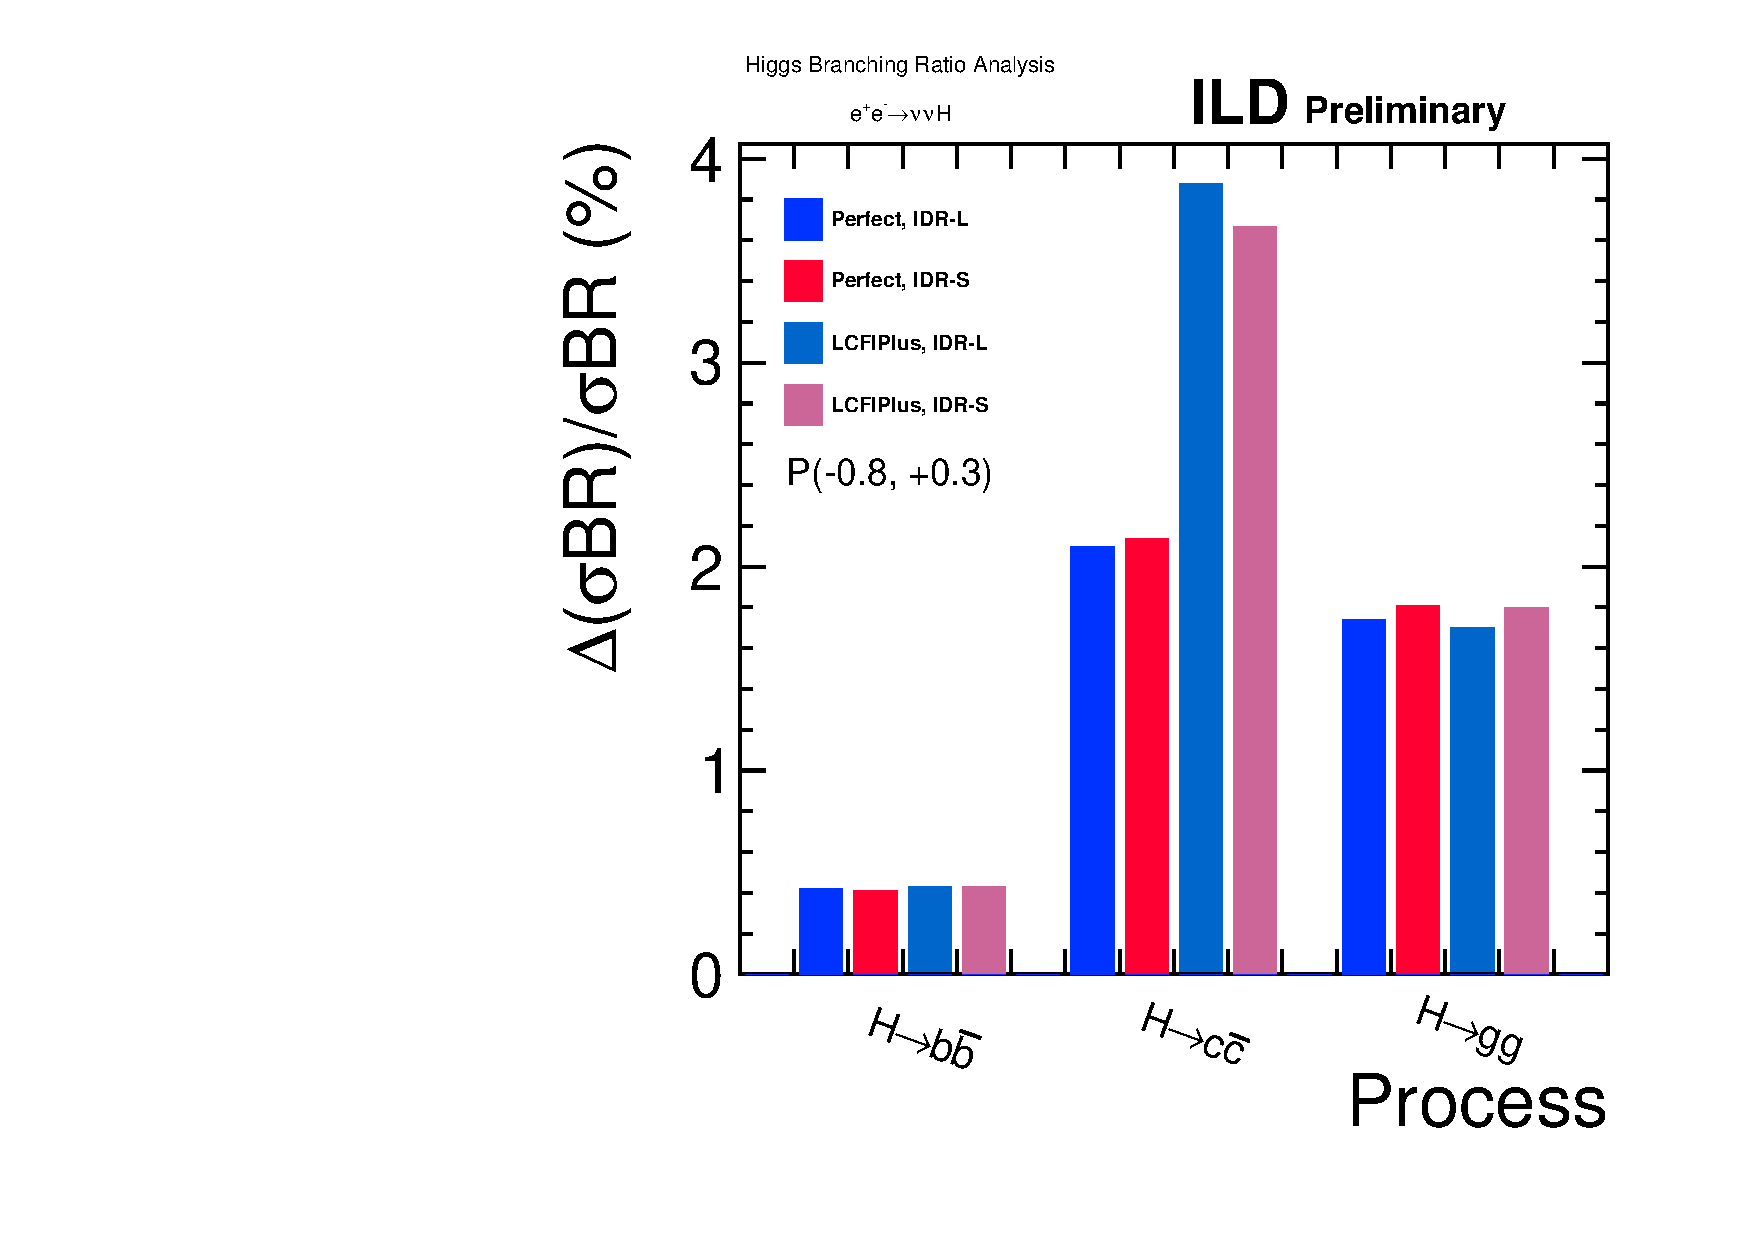
\includegraphics[width=\textwidth]{Performance/fig/IDRplot1.pdf}
 \caption{ \label{fig:Hbbccgg:BR:cheat}}
 \end{subfigure}
%\hspace{0.03\textwidth}
\begin{subfigure}{0.49\hsize} 
 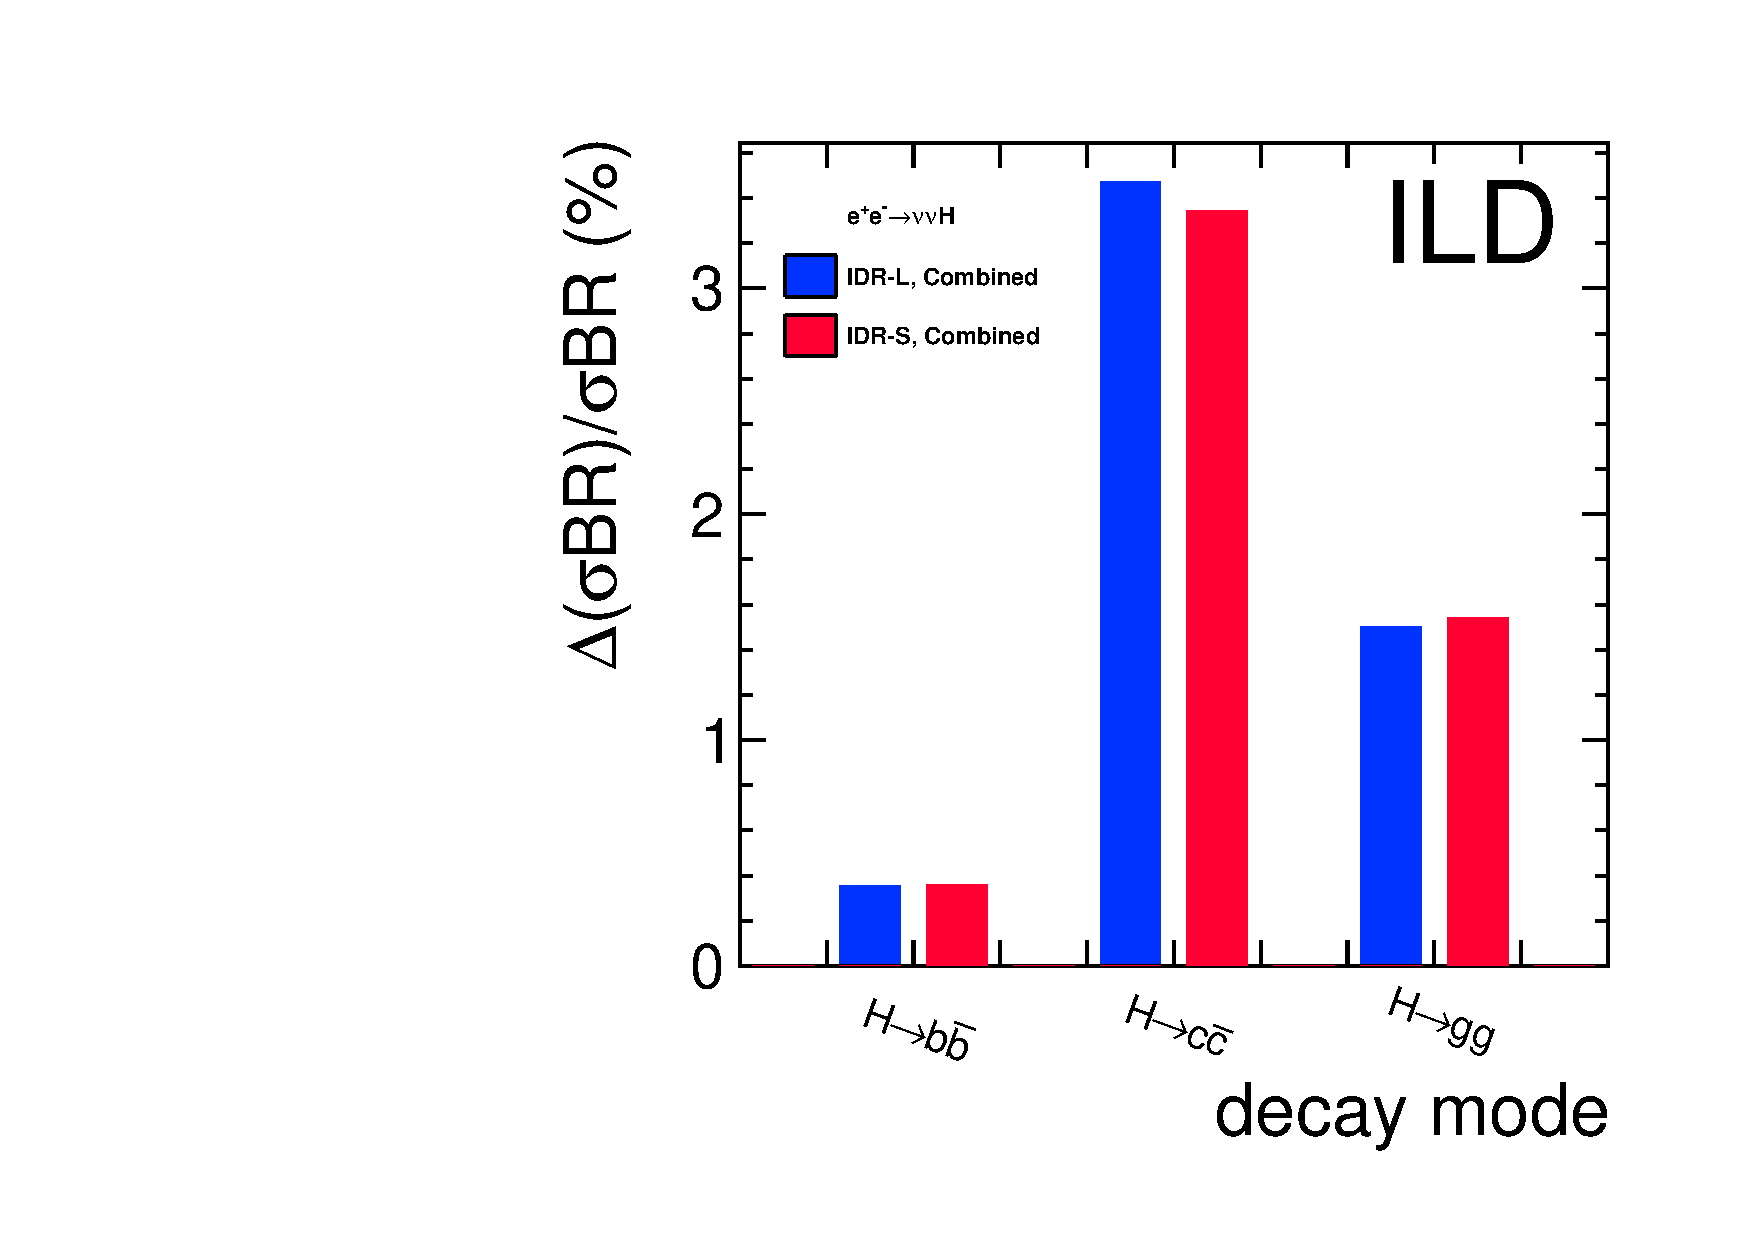
\includegraphics[width=\textwidth]{Performance/fig/IDRplot3.pdf}
 \caption{  \label{fig:Hbbccgg:BR:LS}}
 \end{subfigure}
%\end{center}
\caption{
(a) Comparison of current and ideal flavour tag performance. The precision on $H \to c\bar{c}$ is most sensitive to the actual flavour tag performance.
(b) Comparison of IRD-L and IDR-S for all polarisation configurations combined.
}
\label{fig:Hbbccgg:BR}
\end{figure}

%%%%%%%%%%%%%%%%%%%%%%%%%%%%%%%%%%%%%%%%%%%%%%%%%%%%%%%%%%%%%%%%%%%
\subsection{Higgs Mass from \texorpdfstring{$ZH \to ll b\bar{b}$}{ZH -> llbb}}
\fix{IDR text and plots okayed by Frank Simon(referee). Complete note draft with referee.}

The single most precise method to measure the Higgs mass is the recoil analysis at $\sqrt{s}=250$\,GeV~\cite{Yan:2016xyx}. At $\sqrt{s}$ much higher than the $ZH$ production threshold, the recoil
technique suffers substancially from the increasing amount of ISR and beamstrahlung. In addition, the momenta of the muons from $Z\to \mu\mu$ increase in magnitude and thus are measured less precisely. Still, the data collected at higher centre-of-mass energies can be exploited effectively when using the fully-reconstructable decay modes of the Higgs boson in combination with kinematic constraints from the known initial state. E.g.\ the constraints $\sum_i{p_{i_y}}=0$ and $\sum_i{p_{i_x}}=3.5$\,GeV\footnote{In $x$ direction the initial momentum is not zero due to the crossing angle of the beams, but given by $\sqrt{s} \cdot \sin{14\,\mathrm{mrad}}$.} can replace the measured energies of the Higgs decay products, so that only the {\it angles} of the Higgs decay products and the momenta of the muons from $Z\to\mu^+\mu^-$ enter in the mass reconstruction. Thus the technique is independent of systematic uncertainties as e.g.\ associated with the $b$-jet energy scale. The detailed description of the technique can be found in~\cite{ILDNote:MH}.

The resolutions on the kinematic quantities which enter the Higgs mass reconstruction, namely azimuthal and polar angles of the jets and the muon energy, are compared in Figs.~\ref{fig:mh:res:phi_LS} and~\ref{fig:mh:res:etheta} for IDR-L and IDR-S. For this, 
the jet angles obtained from clustering the MC particles after hadronisation serve as truth reference, so that the detector performance is singled out from other influences.  Figure~\ref{fig:mh:res:phi_hadronisation} illustrates the effect of hadronisation by comparing to the quark-level direction taking IDR-L as example. It shows that the detector resolution (blue histogram, same as in Fig.~\ref{fig:mh:res:phi_LS}) is comparable, but
subdominant to the hadronisation effect (red histogram). While the angular resolutions are very similar for both detector models, the muon energy resolution is worse for the small detector, reflecting the somewhat worse $p_t$ resolution for high-momentum tracks in the central region of the detector, c.f.\ Fig.~\ref{fig:perf:trkres}. 
 
\begin{figure}[htbp]
%\begin{center}
\begin{subfigure}{0.49\hsize} 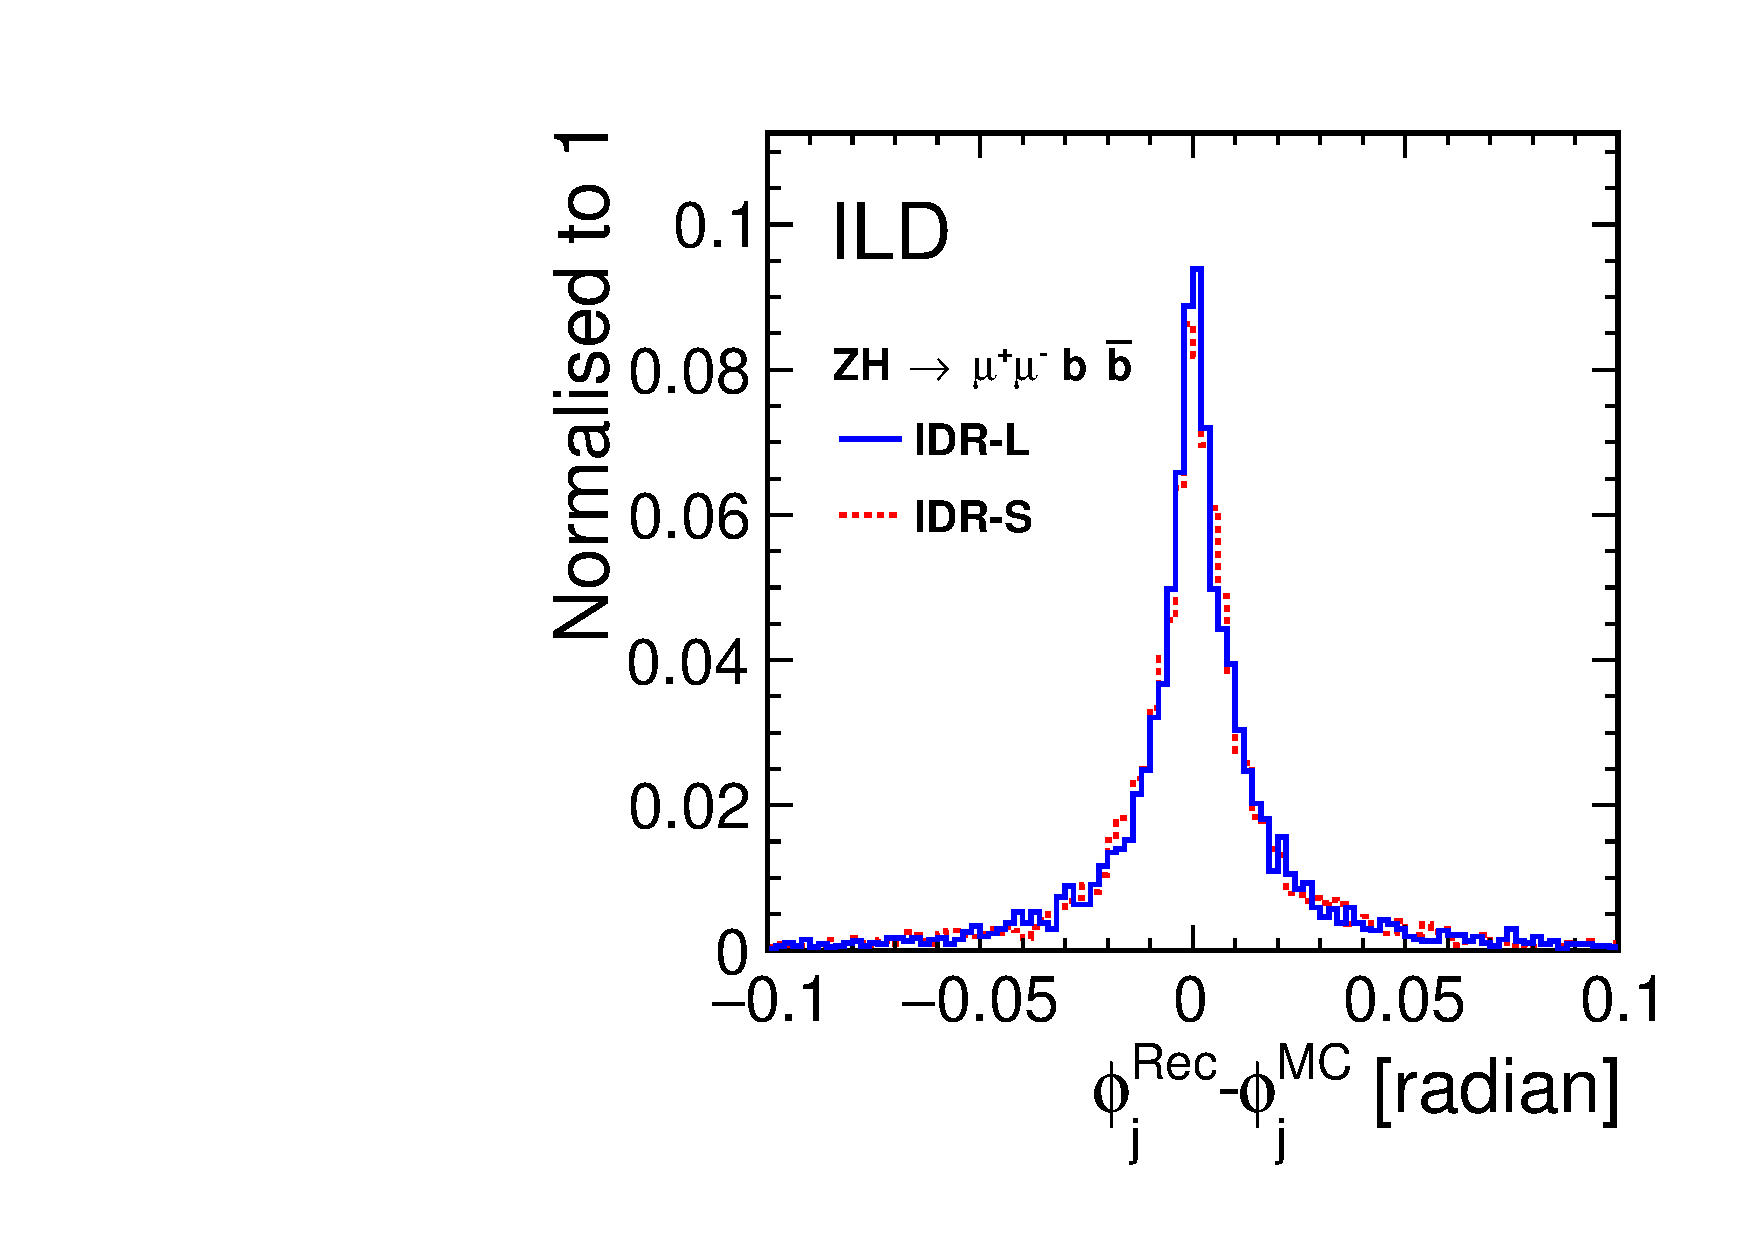
\includegraphics[width=\textwidth]{Performance/fig/phij1h.pdf}
 \caption{ \label{fig:mh:res:phi_LS}}
 \end{subfigure}
%\hspace{0.03\textwidth}
\begin{subfigure}{0.49\hsize} 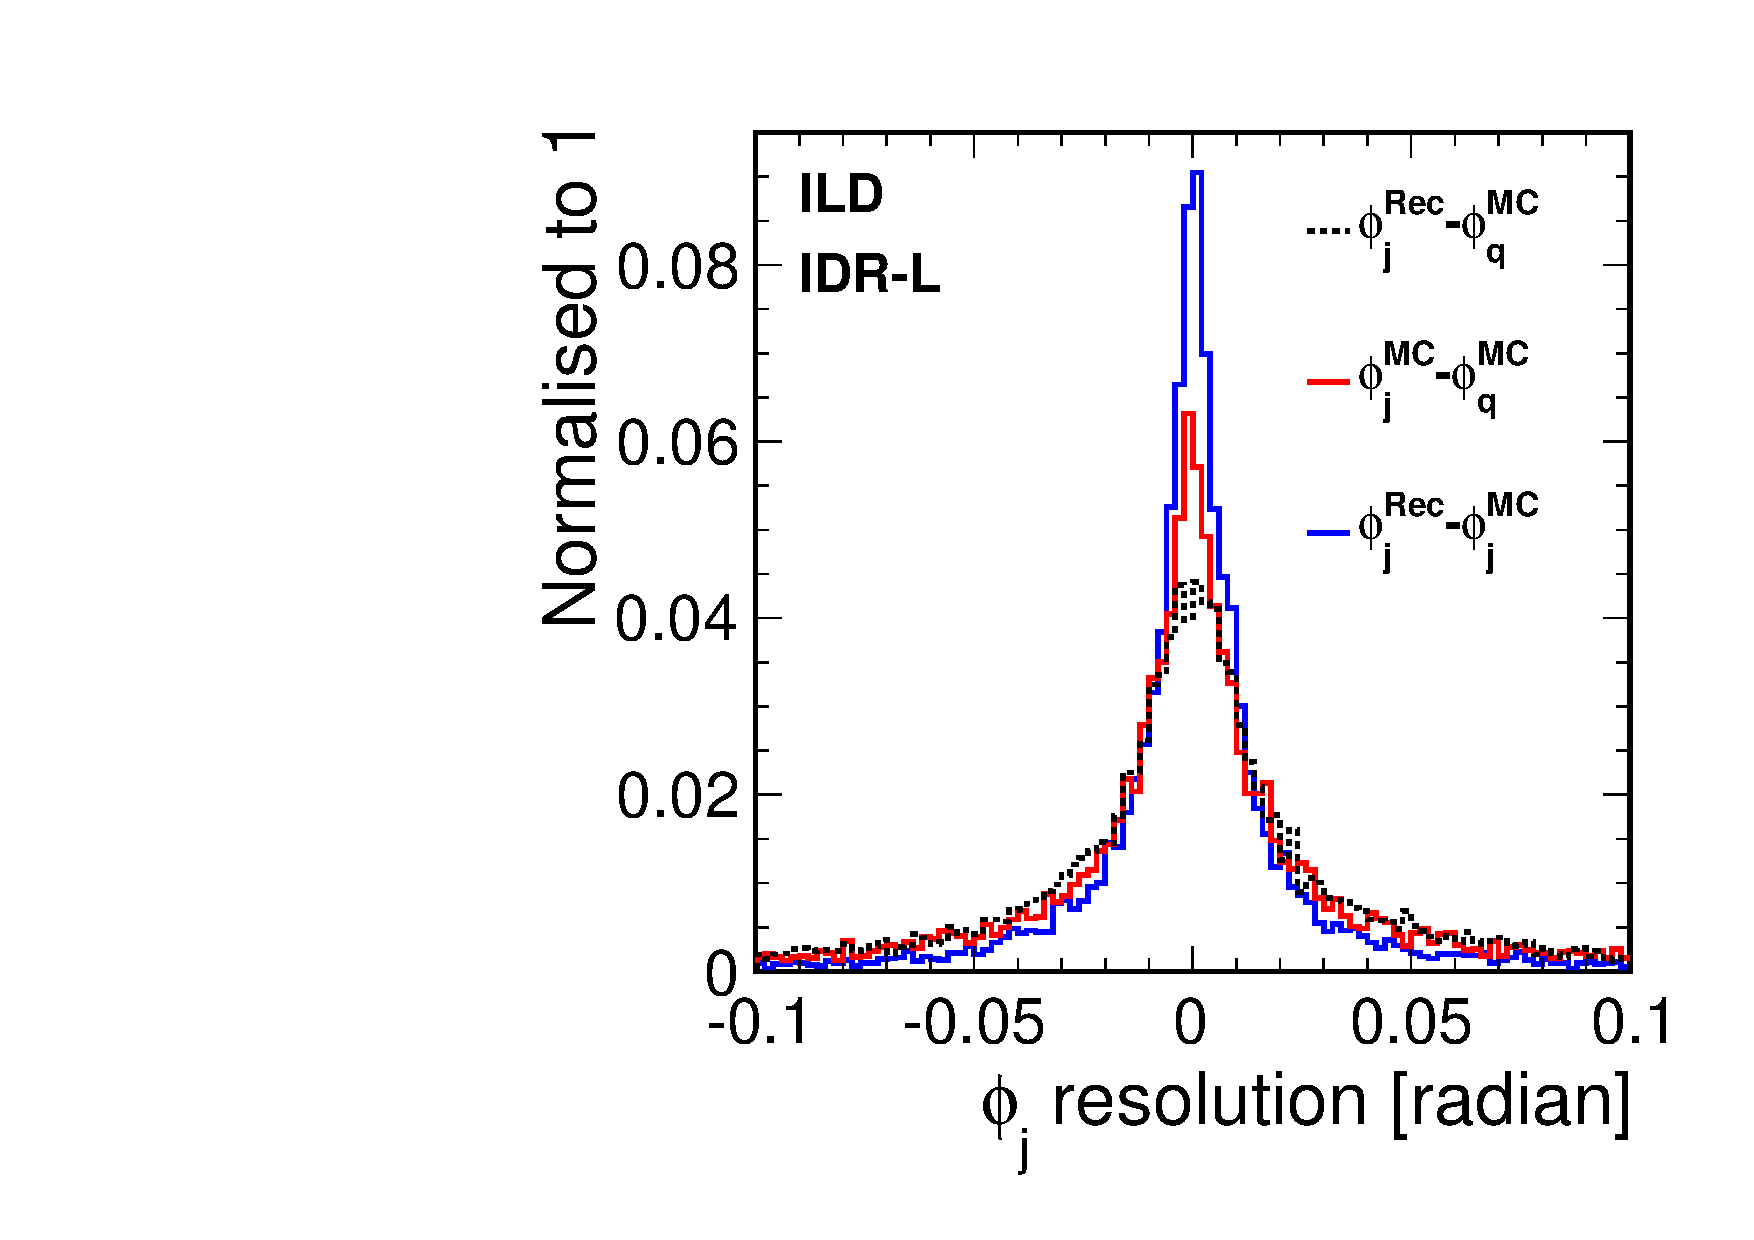
\includegraphics[width=\textwidth]{Performance/fig/phi_res.pdf}
 \caption{  \label{fig:mh:res:phi_hadronisation}}
 \end{subfigure}
%\end{center}
\caption{
(a) Resolution obtained with IDR-L and IDR-S for the jet azimuthal angle
(b) Influence of hadronisation on the jet azimuthal angle
}
\label{fig:mh:res:phi}
\end{figure}

\begin{figure}[htbp]
%\begin{center}
\begin{subfigure}{0.49\hsize} 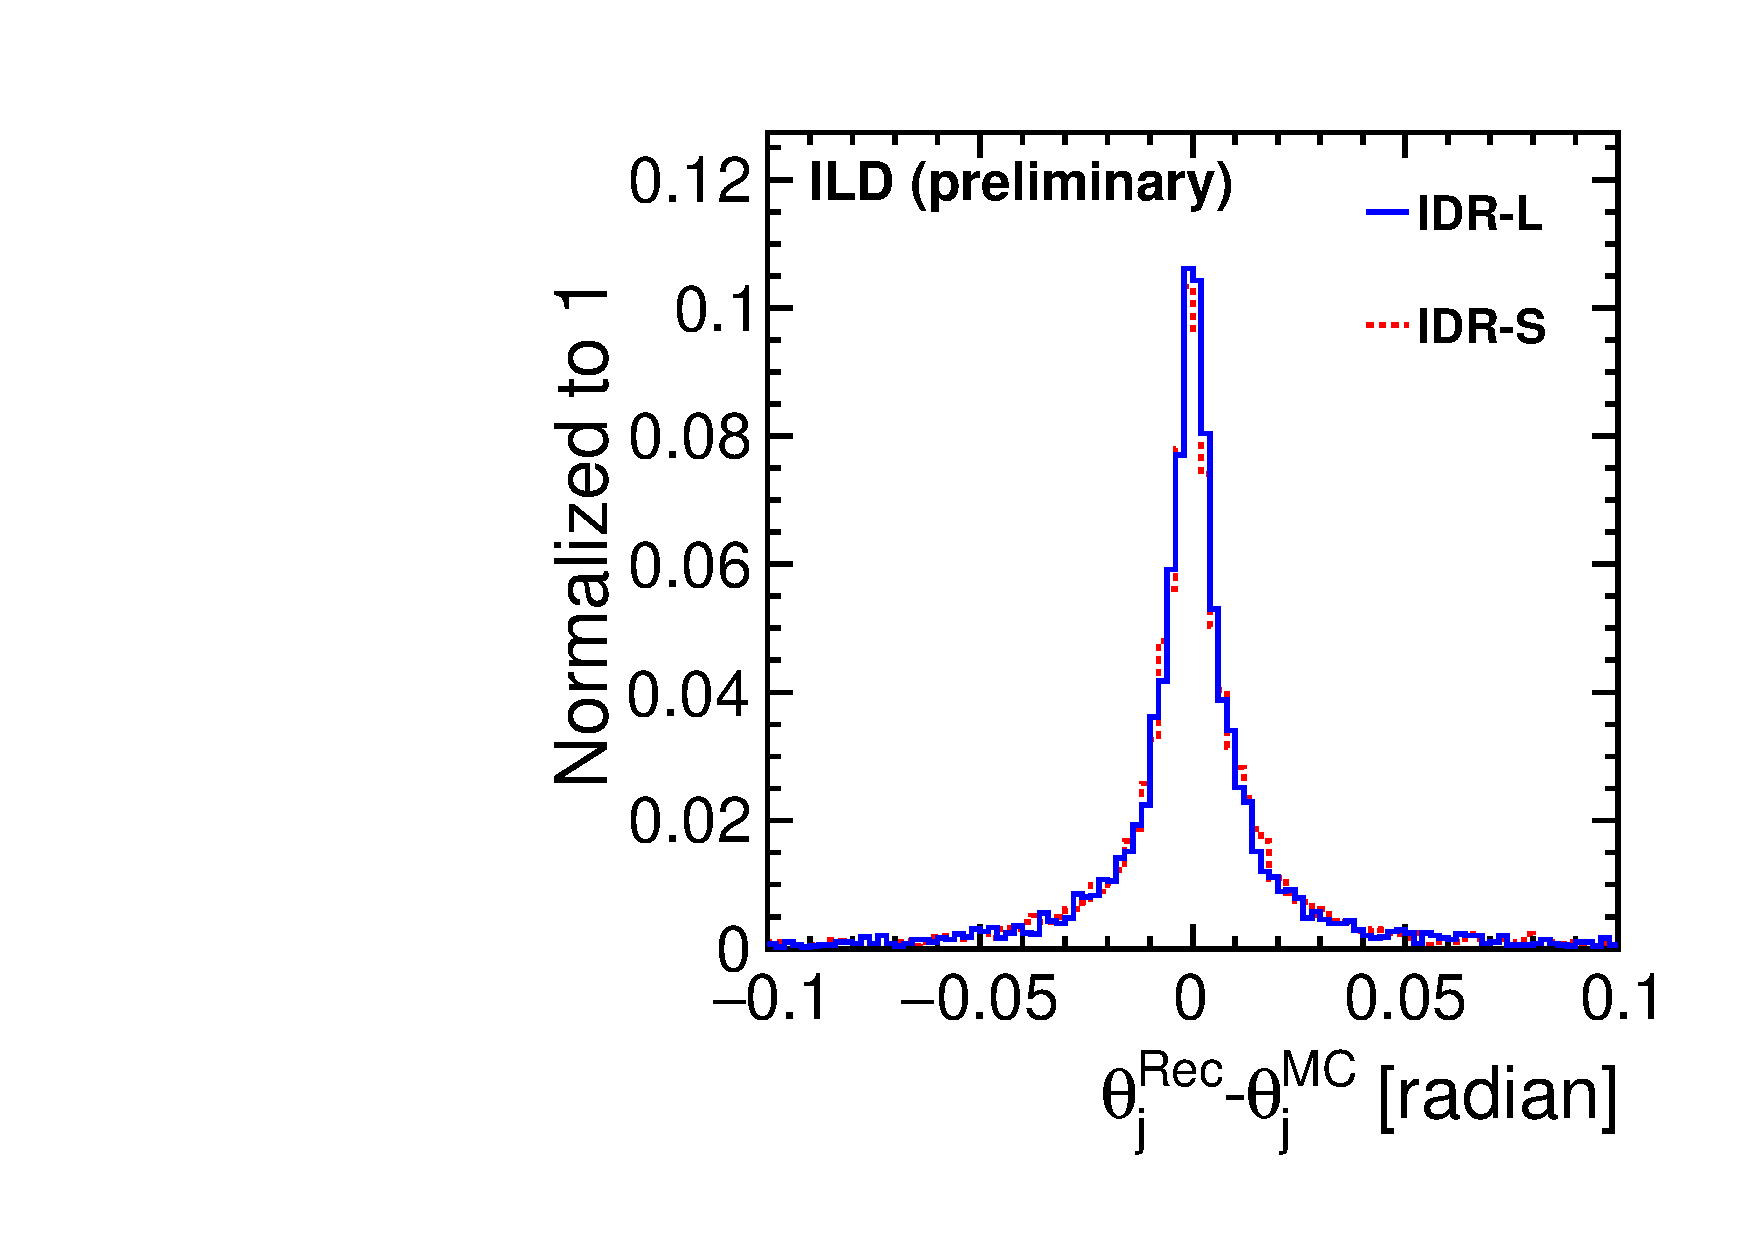
\includegraphics[width=\textwidth]{Performance/fig/thetaj1h.pdf}
 \caption{  \label{fig:mh:res:theta}}
 \end{subfigure}
%\hspace{0.03\textwidth}
\begin{subfigure}{0.49\hsize} 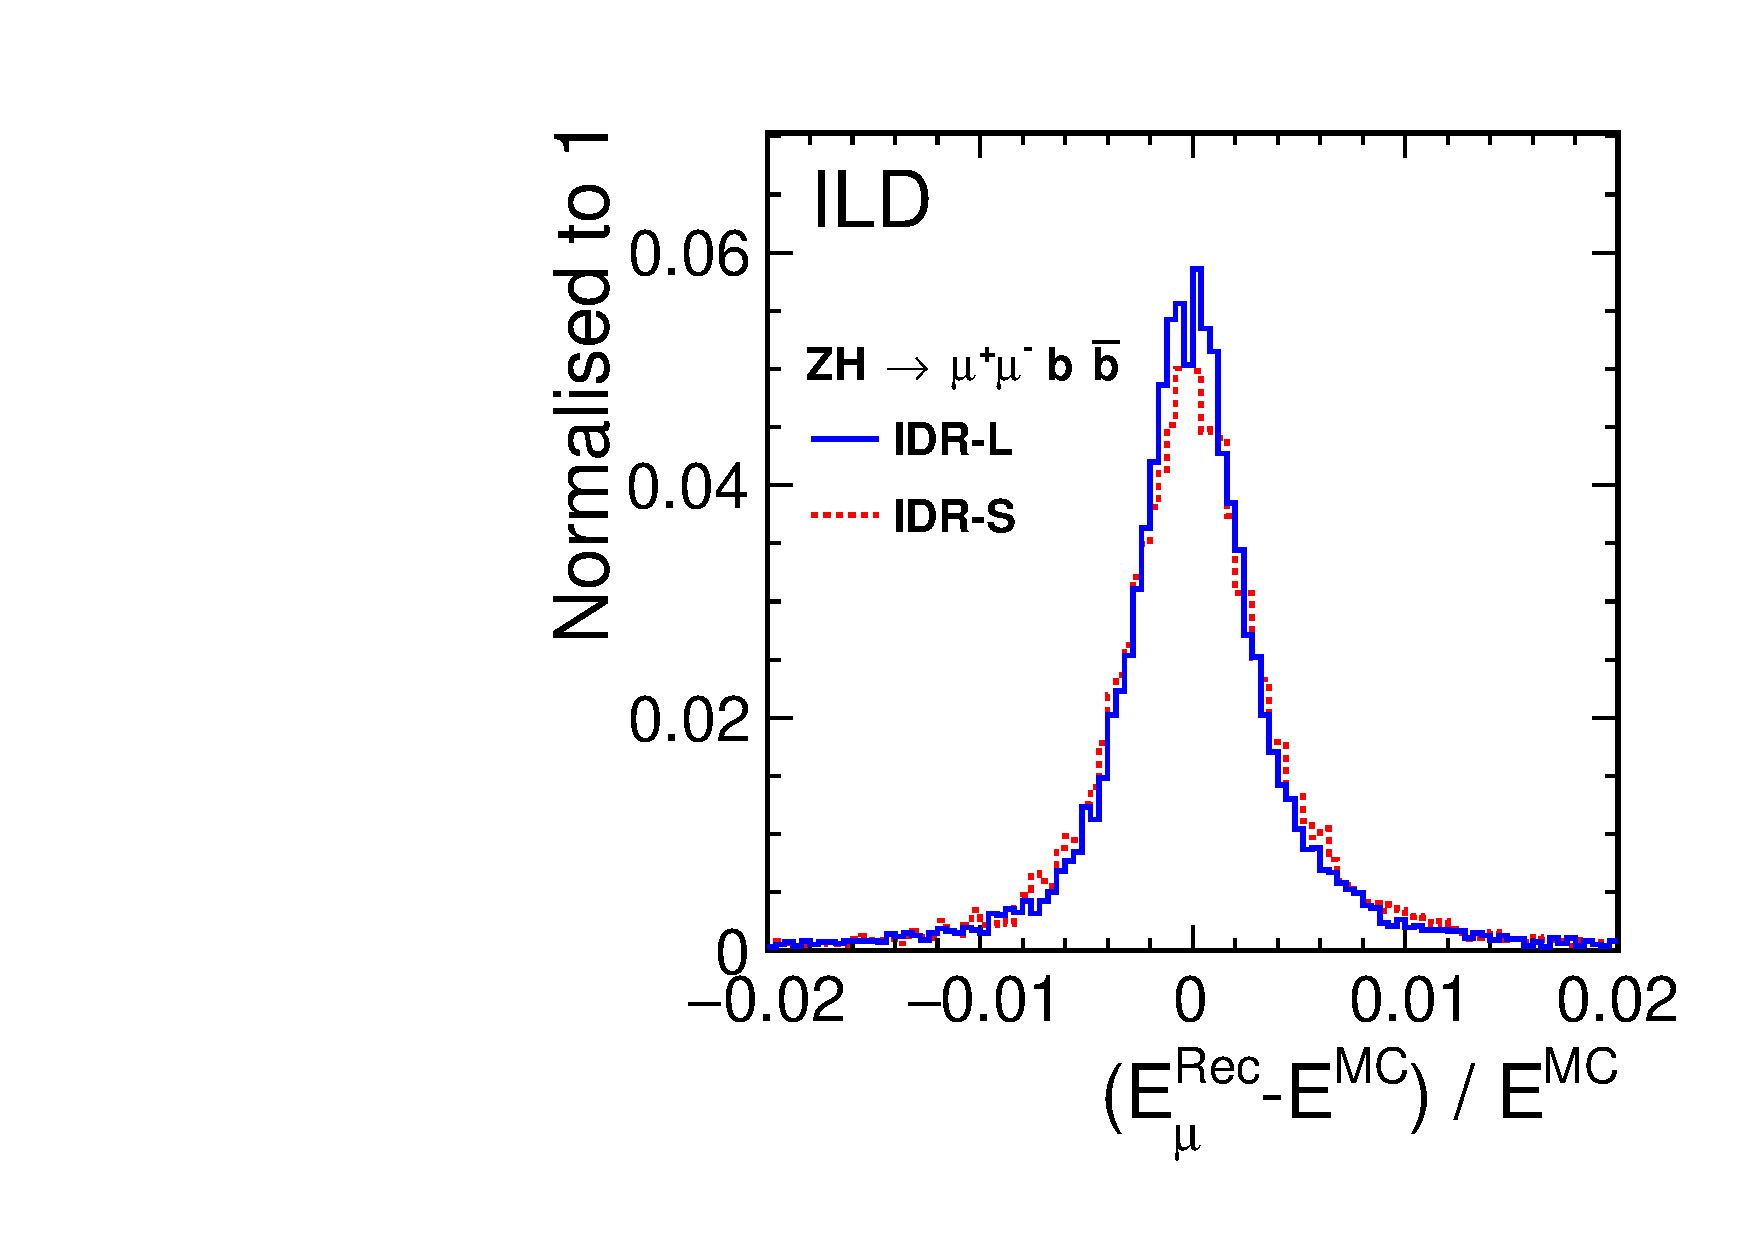
\includegraphics[width=\textwidth]{Performance/fig/elep1.pdf}
 \caption{  \label{fig:mh:res:Elep}}
 \end{subfigure}
%\end{center}
\caption{Resolutions obtained with IDR-L and IDR-S for 
(a) the jet polar angle
(b) the muon energy, after recovery of FSR photons. 
}
\label{fig:mh:res:etheta}
\end{figure}

Figure~\ref{fig:mh:mass} shows the propagation of this effect to the actual physics observable, i.e.\ the reconstructed mass of the Higgs candidates. IDR-L and IDR-S are compared for the muon channel in Fig.~\ref{fig:mh:mass:mumu} and for the electron channel in Fig.~\ref{fig:mh:mass:ee}. In both cases signal and all backgrounds from the SM and other $ZH$ modes are combined, with clear peaks visible around the nominal Higgs and $Z$ boson masses. In particular in the muon channel, the worse momentum resolution of the small detector leads to the peaks being visibly wider. The uncertainty on the Higgs mass is extracted by fitting these distributions following the approach used for the recoil analysis~\cite{Yan:2016xyx}. This results in an uncertainty on the measured Higgs mass of $66$\,MeV in the case of IDR-L and $81$\,MeV for IDR-S, to an increase of about $22\%$.

\begin{figure}[htbp]
%\begin{center}
\begin{subfigure}{0.49\hsize} 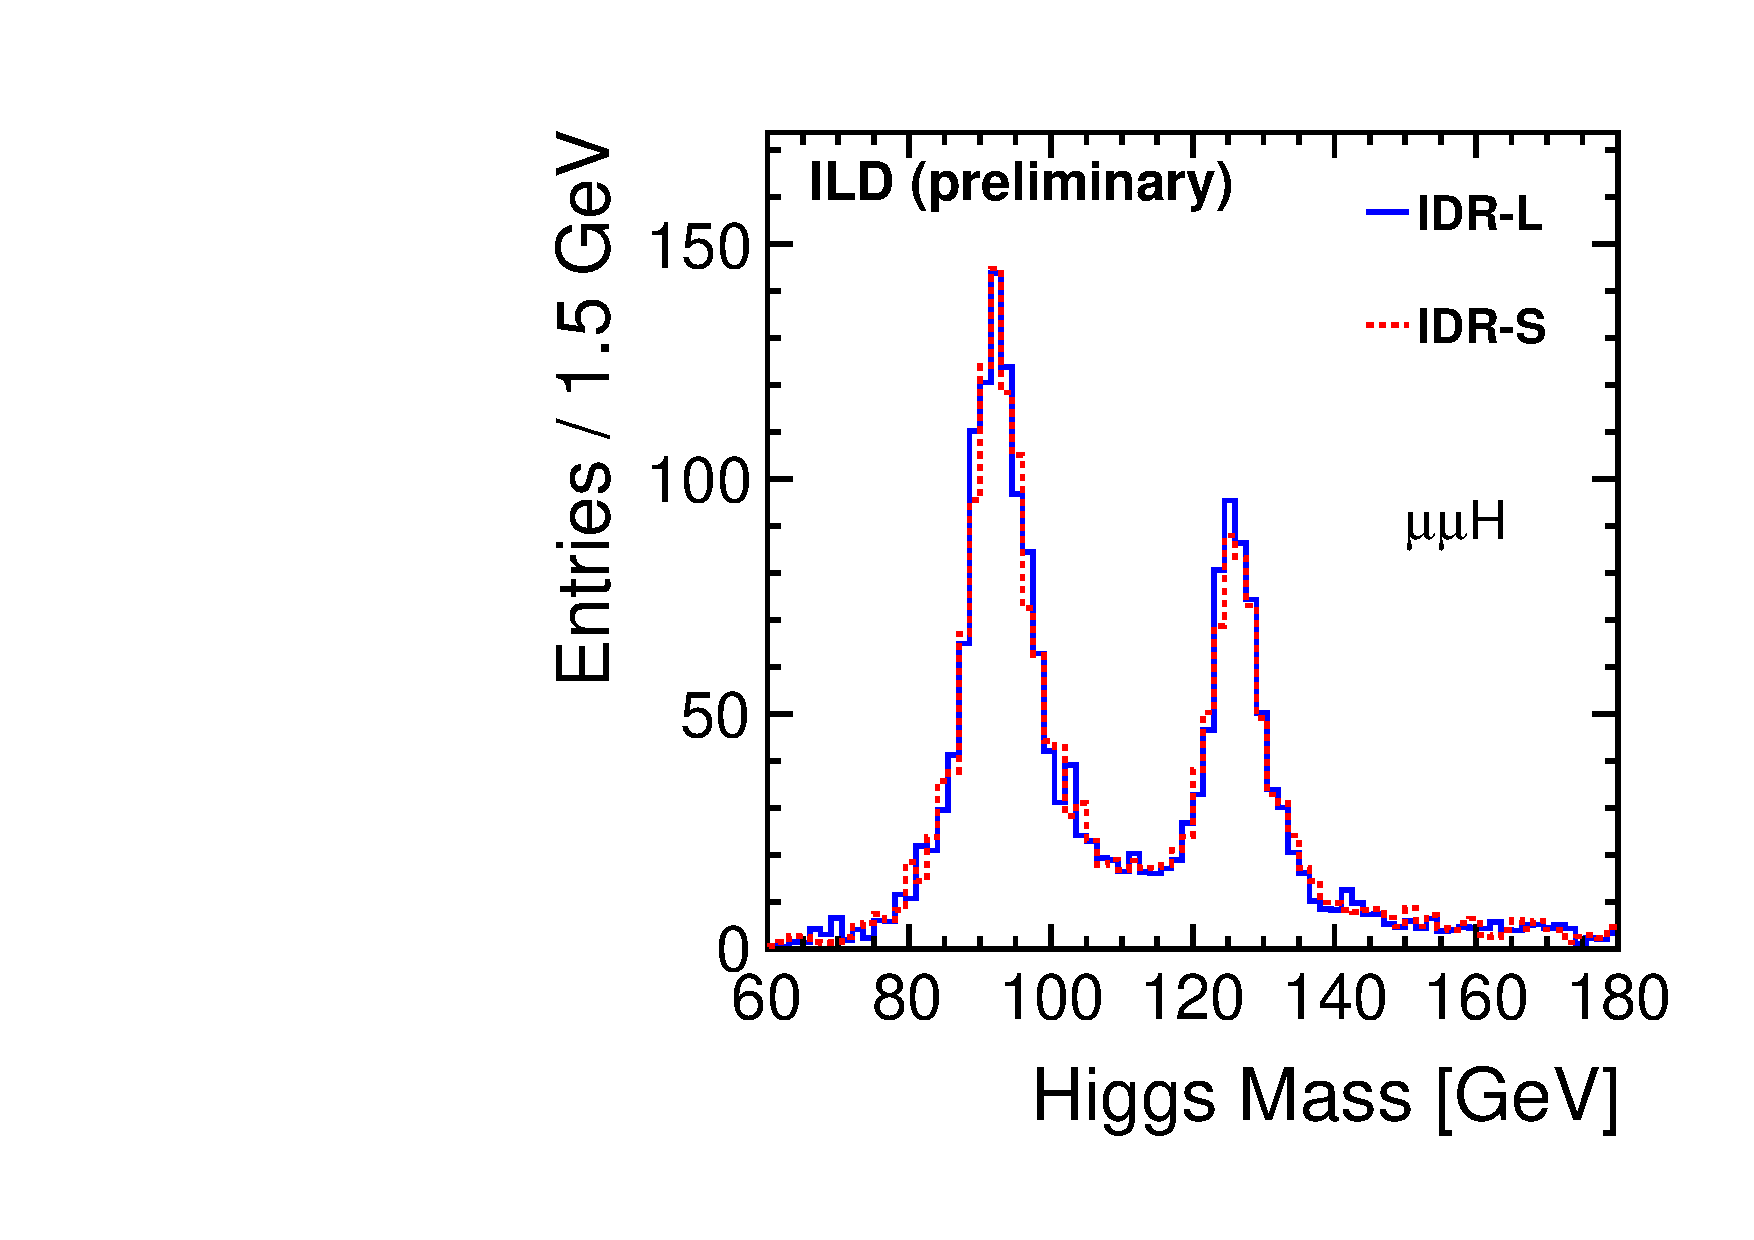
\includegraphics[width=\textwidth]{Performance/fig/mH_e2e2h_bb_eLpR_IDR.pdf}
 \caption{ \label{fig:mh:mass:mumu}}
 \end{subfigure}
%\hspace{0.03\textwidth}
\begin{subfigure}{0.49\hsize} 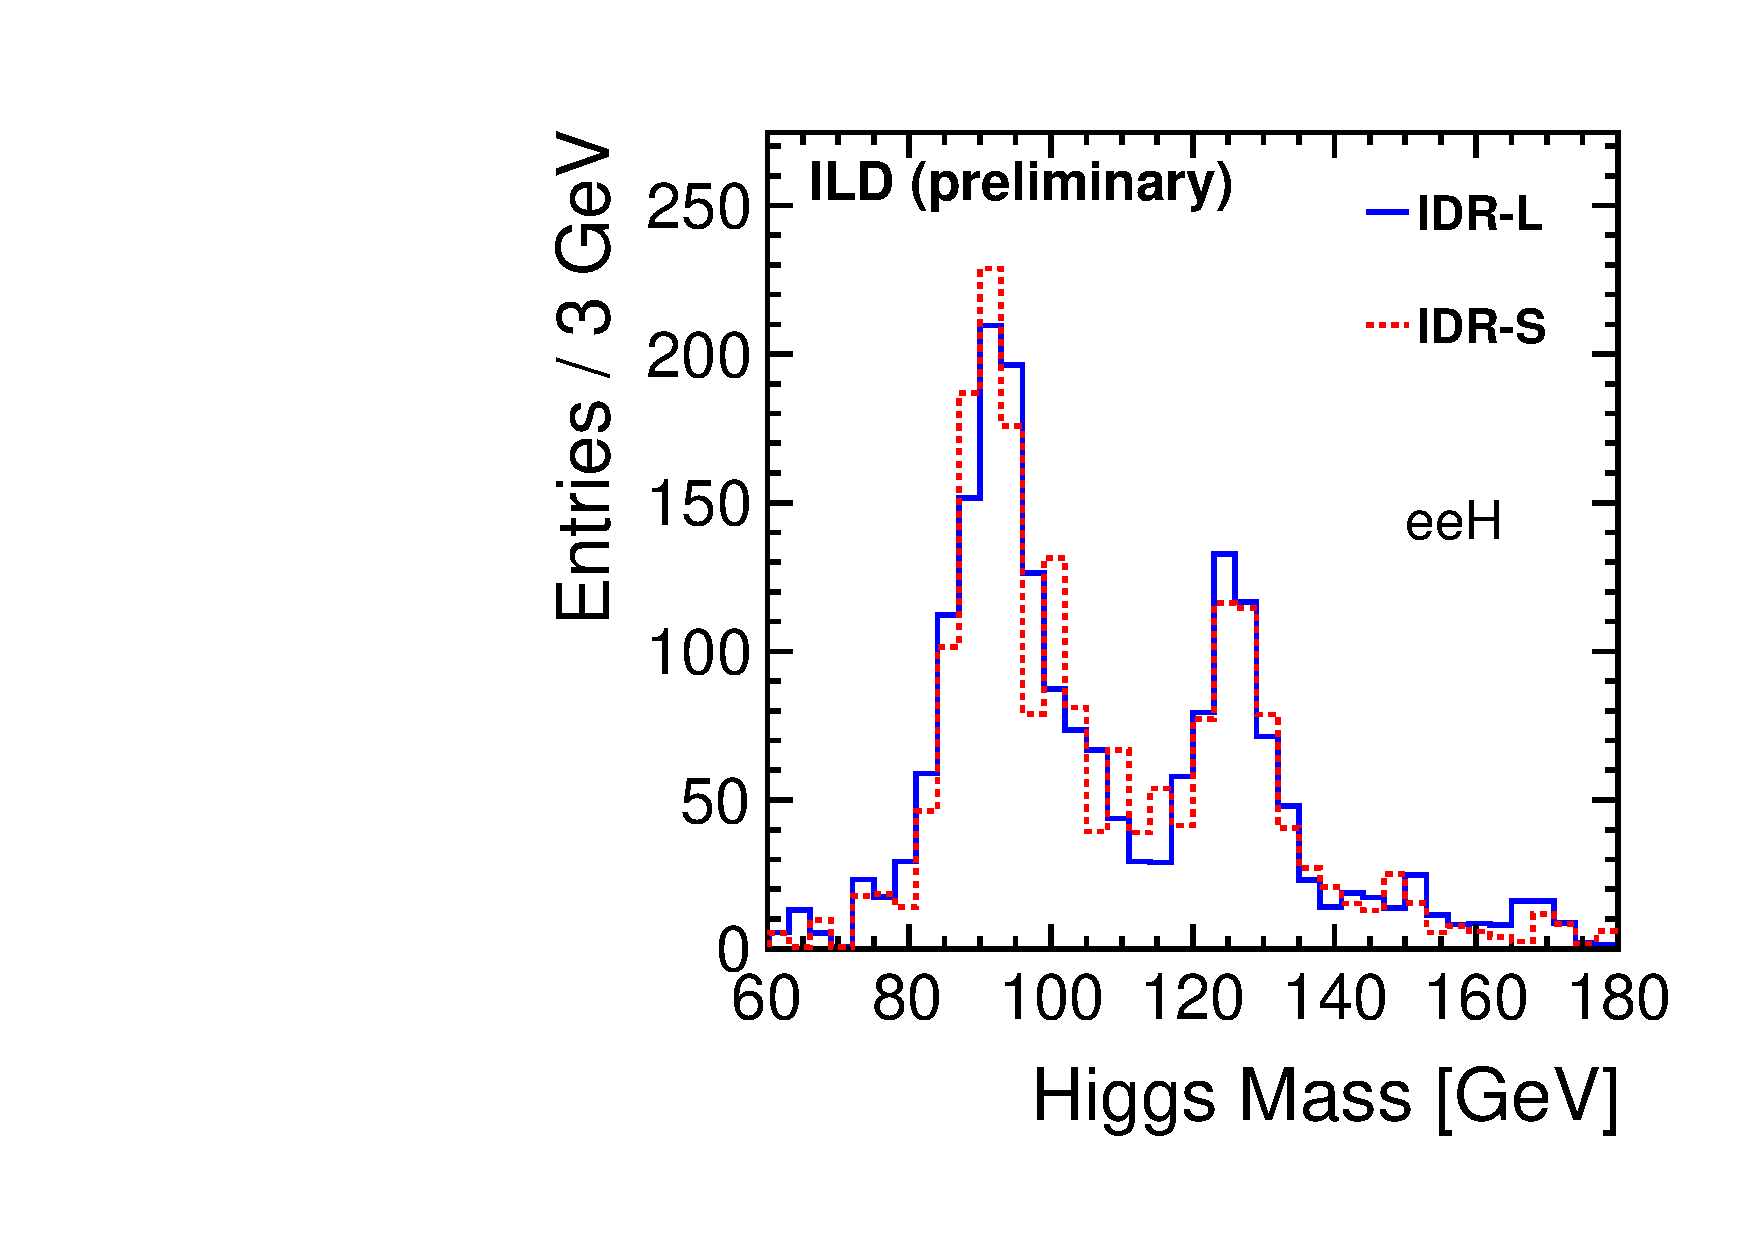
\includegraphics[width=\textwidth]{Performance/fig/mH_e1e1h_bb_eLpR_IDR.pdf}
 \caption{  \label{fig:mh:mass:ee}}
 \end{subfigure}
%\end{center}
\caption{reconstructed Higgs mass distribution for signal and background for IDR-L and IDR-S
(a) muon channel
(b) electron channel (here with limited MC statistics, thus a reduced number of bins)
}
\label{fig:mh:mass}
\end{figure}


%%%%%%%%%%%%%%%%%%%%%%%%%%%%%%%%%%%%%%%%%%%%%%%%%%%%%%%%%%%%%%%%%%%
\subsection{Branching Ratio of \texorpdfstring{$H \to \mu^+\mu^-$}{H -> mm}}
\fix{everything done!}

In the SM, the decay of the Higgs boson into a pair of muons is a very rare decay, with a branching ratio of $2.2 \times 10^{-4}$. In order to identify this small signal, the achievable mass resolution, thus the precision to which the momenta of the two muons are measured, plays a crucial role. For the purpose of detector benchmarking, we consider only 
$\sigma(\nu\bar{\nu} H)\times BR(H\to \mu^+\mu^-)$ as observable, which isolates best the effect of the muon momentum resolution.

The selection~\cite{ILDNote:Hmumu} targets events with substancial missing four-momentum plus 
two well-reconstructed, oppositely charged muons. Kinematic and angular variables are exploited in an MVA analysis. Figure~\ref{fig:Hmumu:mass} shows the di-muon invariant mass distribution for all selected signal events. In case of the small the detector model, the mass peak is about $10\%$ wider than for the large detector. This originates from the combination of the muons from the Higgs decay being high-energetic and rather central, plus the better momentum resolution of the large detector for high-momentum tracks in the barrel. 
This effect is seen more clearly in Fig.~\ref{fig:Hmumu:sigma}, which compares the event-by-event resolution of the di-muon invariant mass for the selected signal events with both muons in the barrel region of the detector ($|\cos{\theta}| < 0.7$). 


For the $500$\,GeV data set of the H20 scenario, the asymptotic precision on cross section times branching ratio for the case of $100\%$ efficiency and no backgrounds would be 13\%.  
\begin{figure}[htbp]
%\begin{center}
\begin{subfigure}{0.49\hsize}  
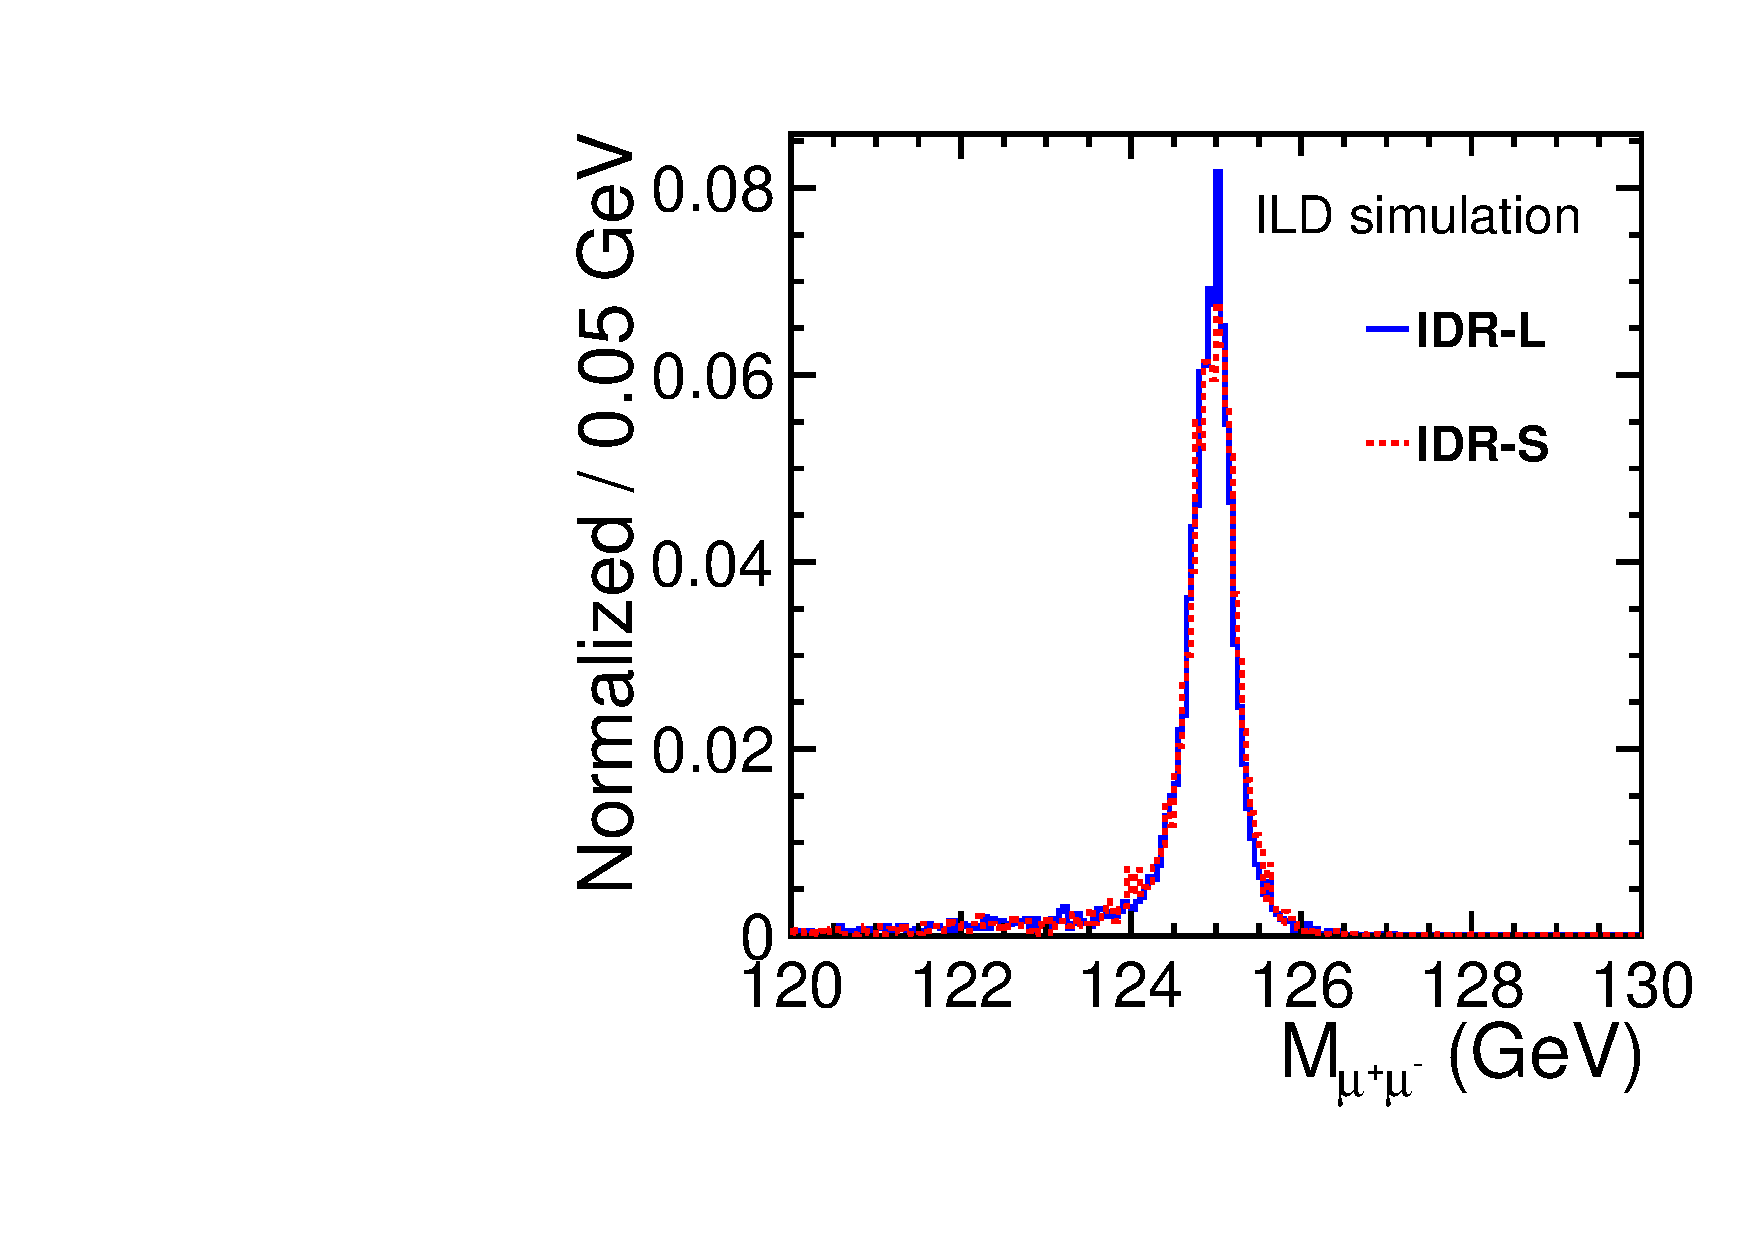
\includegraphics[width=\textwidth]{Performance/fig/mumu_mass.pdf}
\caption{ \label{fig:Hmumu:mass}}
 \end{subfigure}
%\hspace{0.03\textwidth}
\begin{subfigure}{0.49\hsize}  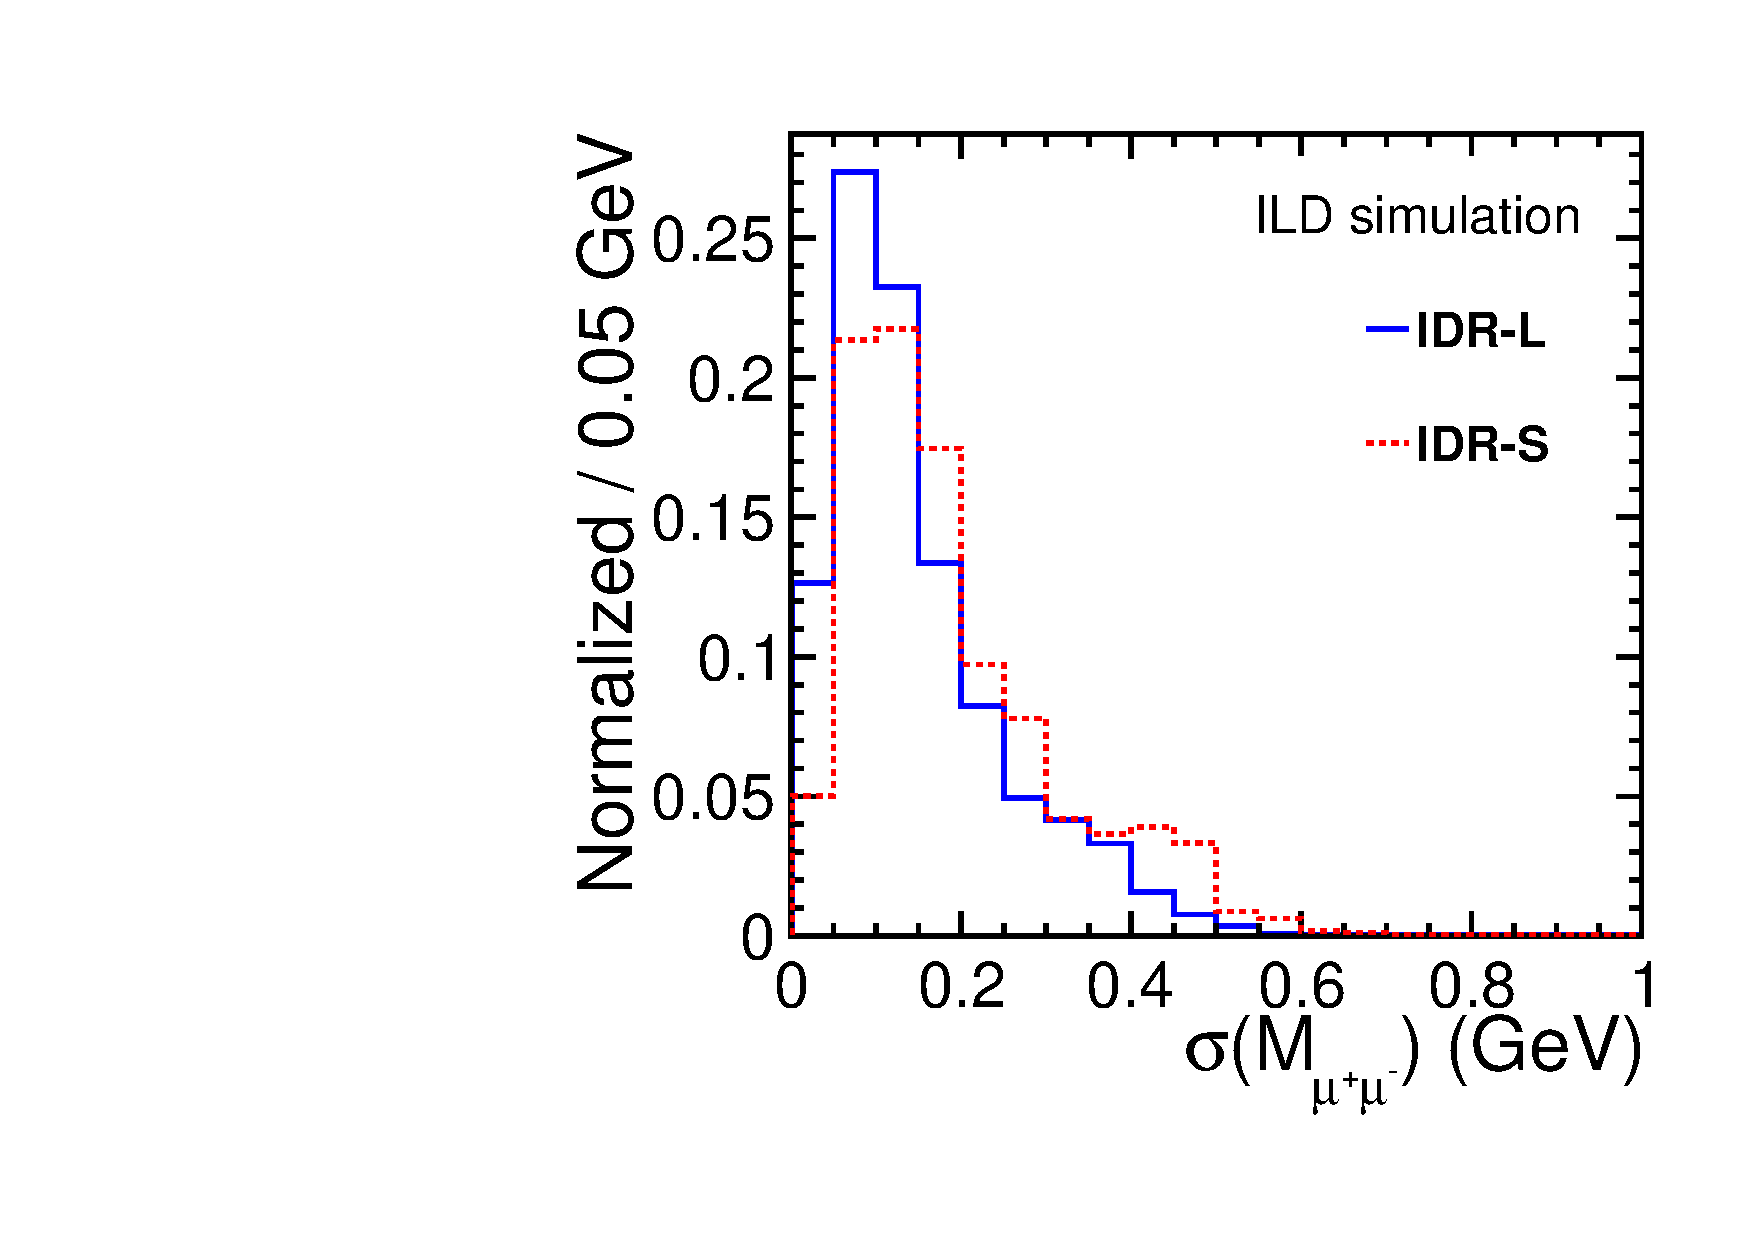
\includegraphics[width=\textwidth]{Performance/fig/sigma_mumu_mass_07.pdf}
 \caption{  \label{fig:Hmumu:sigma}}
 \end{subfigure}
%\end{center}
\caption{$H \to \mu^+\mu^-$ benchmark:
(a) di-muon invariant mass for all selected signal events
(b) mass resolution for the case that both muons are in the barrel region of the detector ($|\cos{\theta}| < 0.7$)
}
\label{fig:Hmumu}
\end{figure}

After the event selection, about $33$ signal events, corresponding to a selection efficiency of $58\%$, remain over a evenly distributed background of about $1100$ events (counted in a mass window between $120$ and $130$\,GeV). Finally, the expectation values for the number of signal events observable above the backgrounds as well as for its uncertainty are obtained from many toy MC fits to the di-muon invariant mass spectrum~\cite{ILDNote:Hmumu}. The obtained precisions on $\sigma(\nu\bar{\nu} H)\times BR(H\to \mu^+\mu^-)$ are $40.2$\% for IDR-L and $41.3$\% for IDR-S. The relative difference of $2.8$ is consistent with the expectation of a $\sim 10\%$ difference in the signal peak width over a flat background. Either number, however, is about a factor $3$ worse than the asymptotic precision for the case of $100\%$ efficiency and no backgrounds, which would be 13\%. The difference is wastly dominanted by the remaining ``irreducible'' backgrounds with two muons and two neutrinos from $W$ pairs decaying either directly to muons or via tau-leptons. While there is certainly room for improvement in rejecting these backgrounds, this will factorize from the impact of the signal peak width, as long as the background remains flat in the discriminating variable. 
 


%%%%%%%%%%%%%%%%%%%%%%%%%%%%%%%%%%%%%%%%%%%%%%%%%%%%%%%%%%%%%%%%%%%
\subsection{Sensitivity to \texorpdfstring{$H \to $ invisible}{H -> invisible}}
\fix{Yu and Marcel (referee) okayed IDR draft, note incomplete}

The decay of the Higgs boson into invisible particles is of particular interest because
it could give important clues about the nature of Dark Matter. As a detector benchmark for testing the impact of the jet energy resolution, in particular the hadronic decay mode of the $Z$ boson is considered here. Thus the physics observable will be the upper limit on $\sigma(q\bar{q} H)\times BR(H \to \mbox{inv.})$.

The event selection~\cite{ILDNote:Hinv} targets events which are consistent with  a di-jet plus missing four-momentum topology, where the di-jet invariant mass should be compatible with the $Z$ boson mass. The jet finding step also serves to reject PFOs from overlay of $\gamma\gamma \to $ low-$p_t$ hadron events. The final discriminating variable is the
invariant mass of the ``invisible'' four-momentum recoiling against the $Z$ boson. 

\begin{figure}[htbp]
%\begin{center}
\begin{subfigure}{0.49\hsize} 
 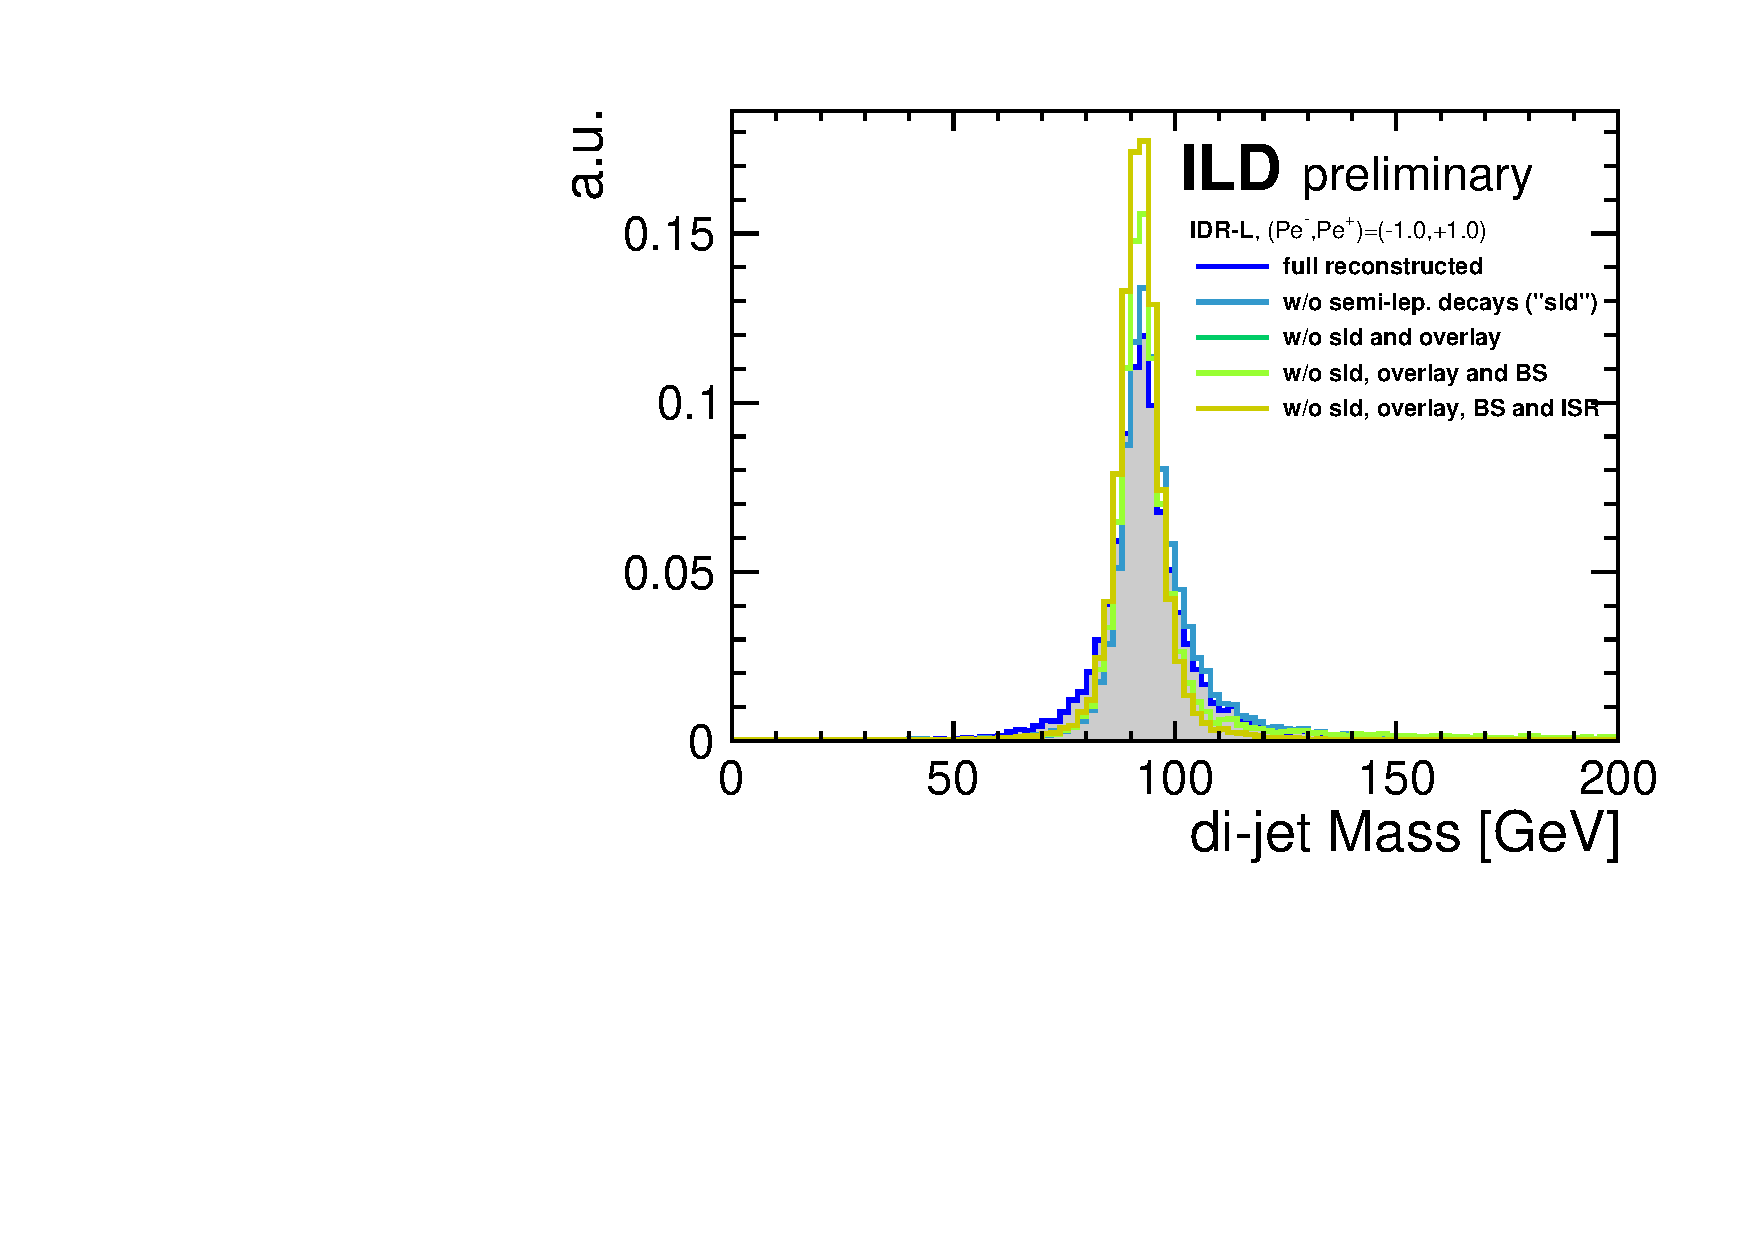
\includegraphics[width=\textwidth]{Performance/fig/compare_cheat_mjj_l5_lr.pdf}
 \caption{ \label{fig:Hinv:cheat:mjj}}
 \end{subfigure}
%\hspace{0.03\textwidth}
\begin{subfigure}{0.49\hsize} 
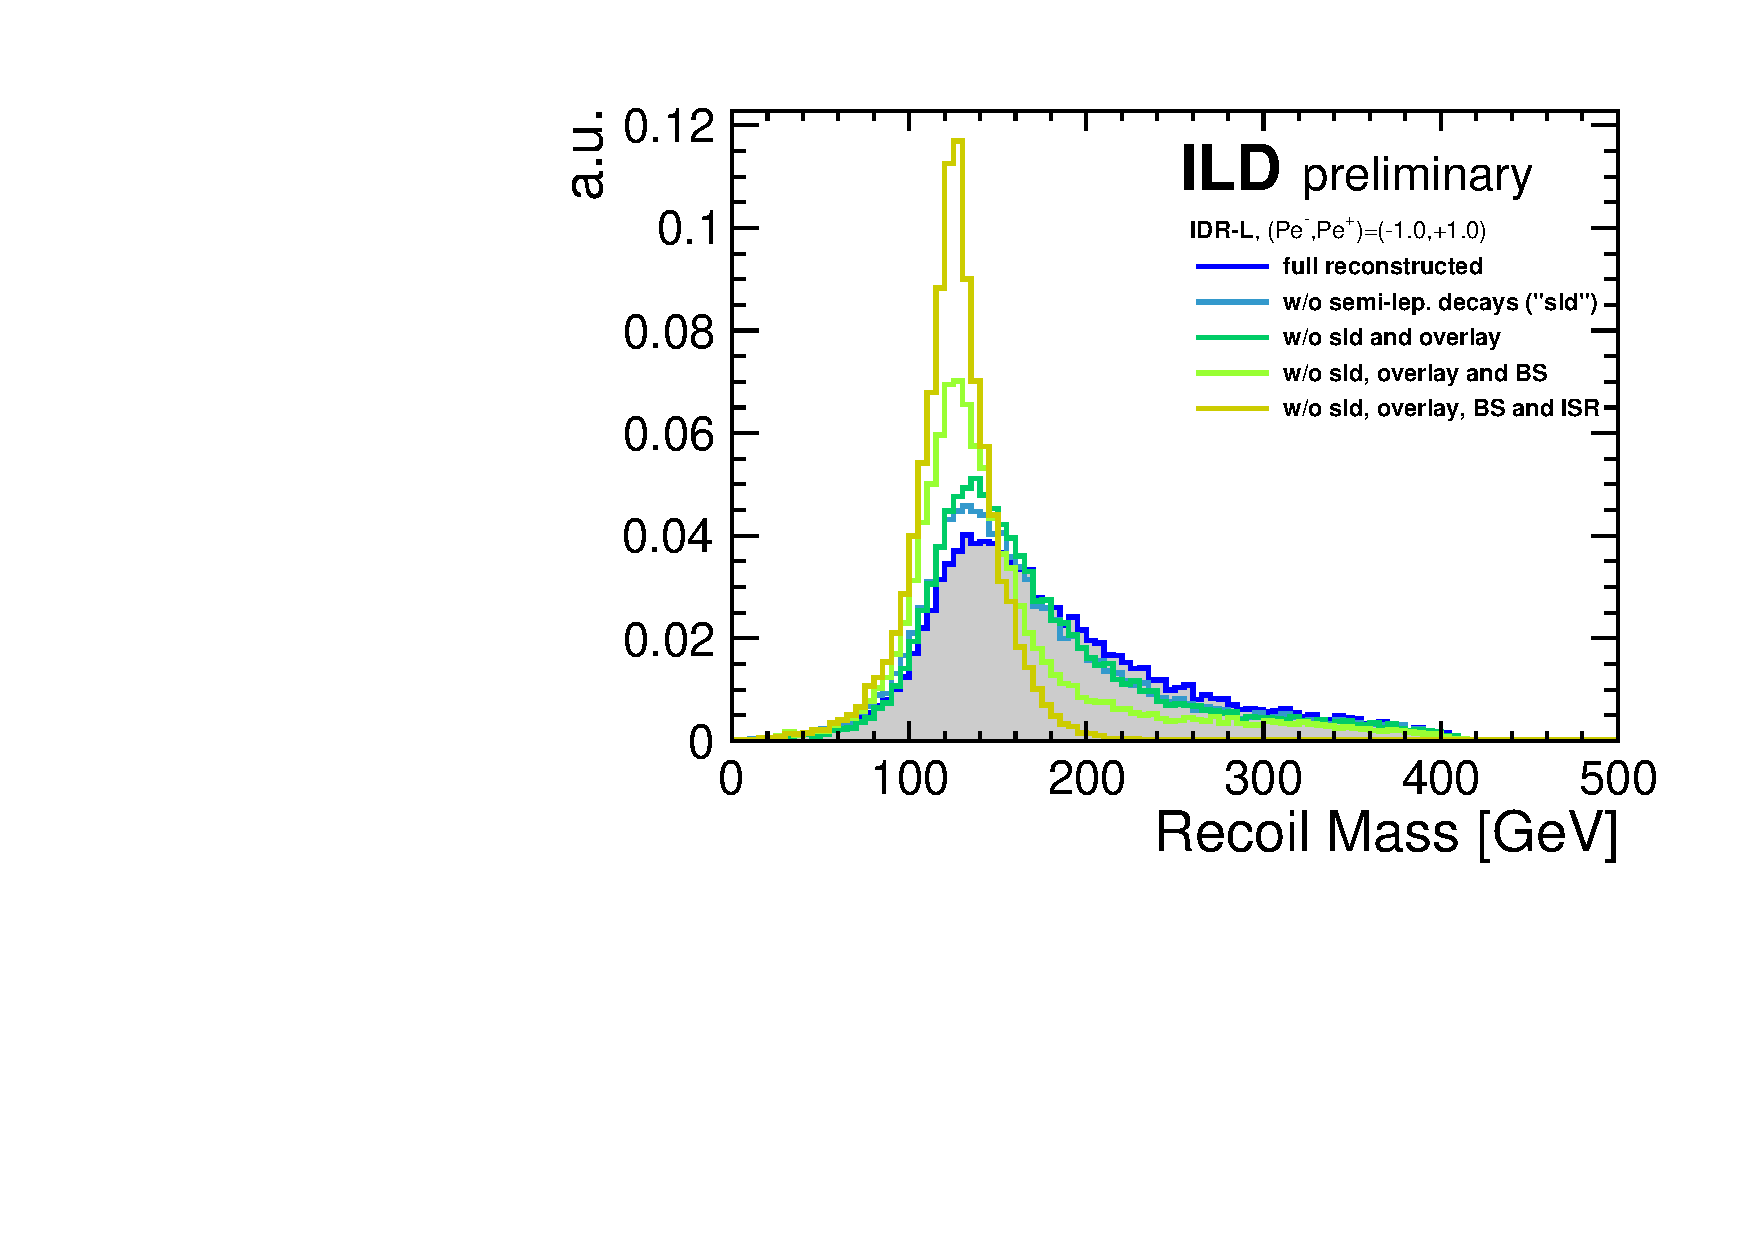
\includegraphics[width=\textwidth]{Performance/fig/compare_cheat_mrec_l5_lr.pdf}
 \caption{  \label{fig:Hinv:cheat:mrec}}
 \end{subfigure}
%\end{center}
\caption{Impact of various effects on
(a) the invariant di-jet mass and
(b) the recoil mass,
shown for the example of the large detector model.
}
\label{fig:Hinv:cheat}
\end{figure}

\begin{figure}[htbp]
%\begin{center}
\begin{subfigure}{0.49\hsize} 
 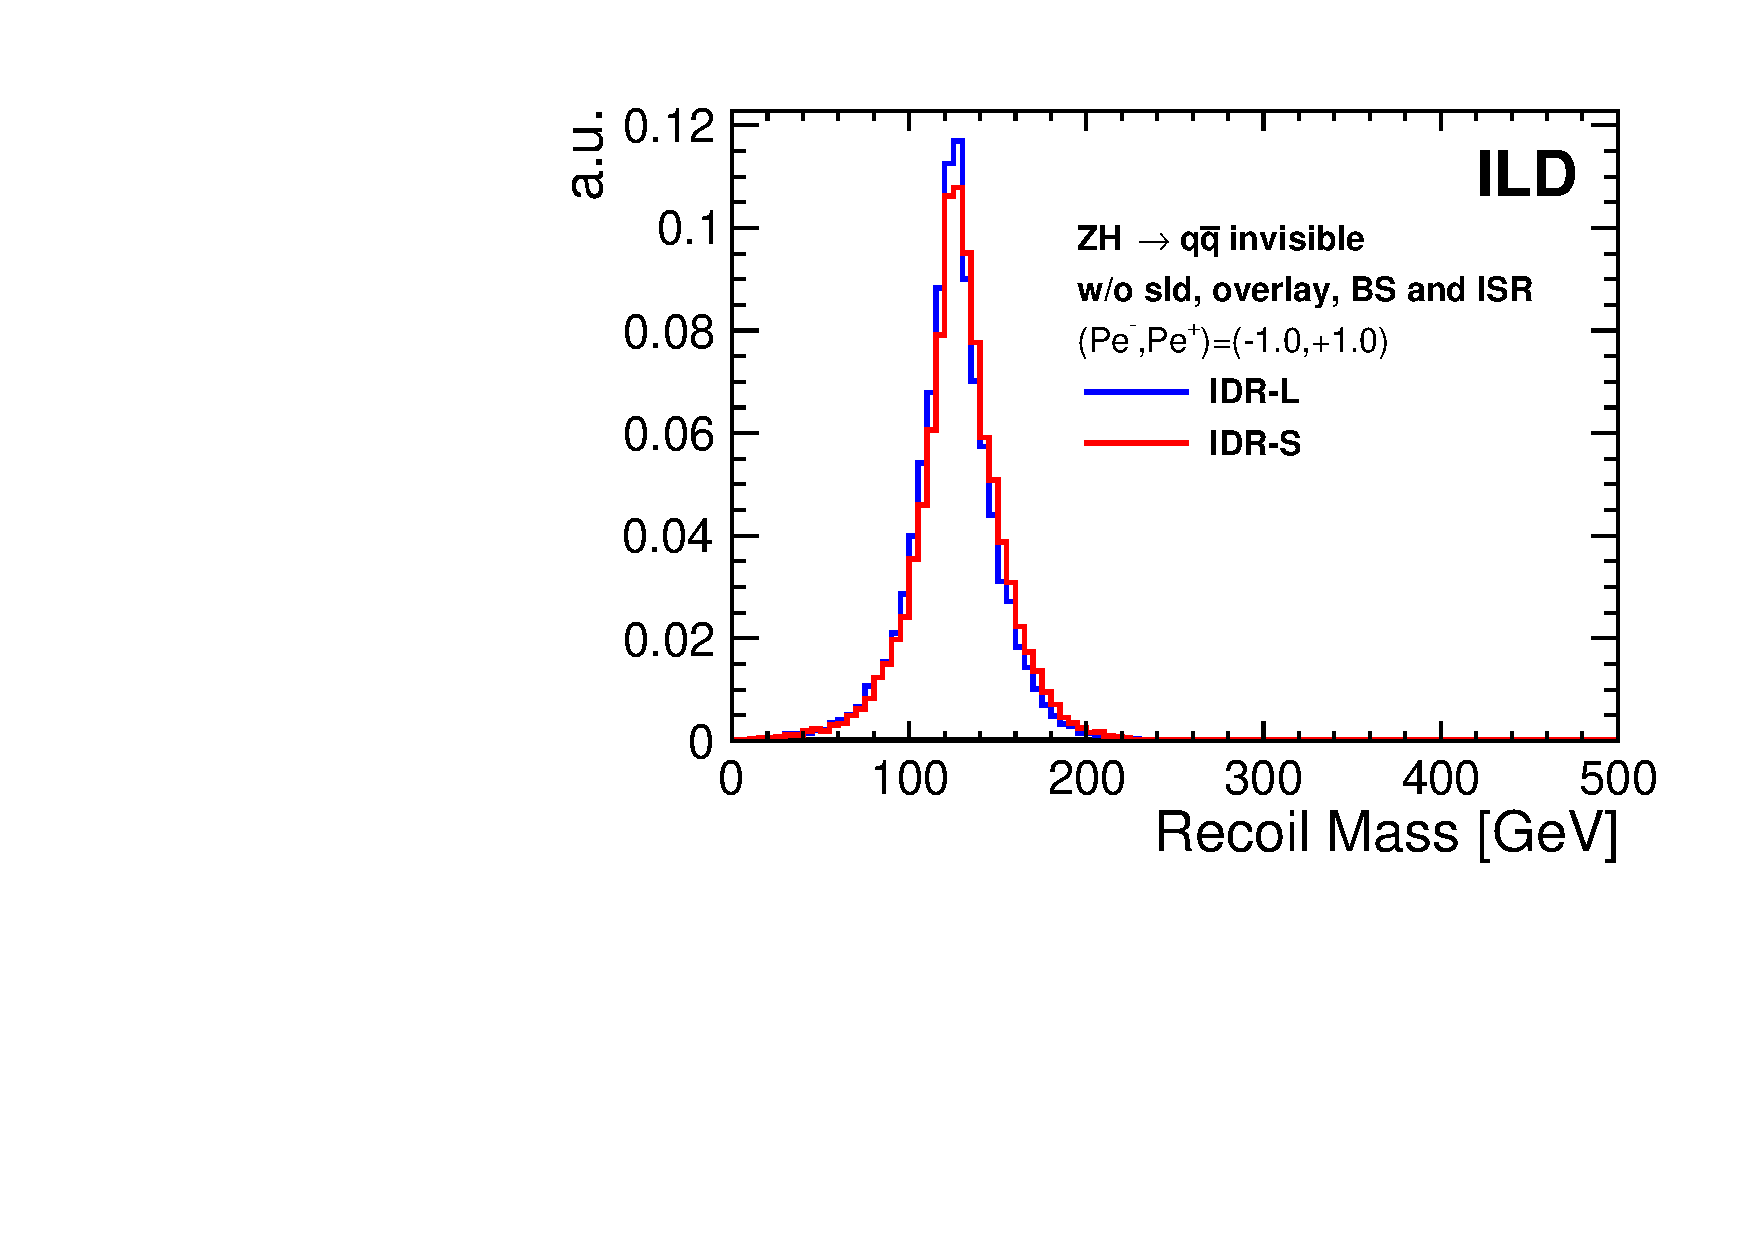
\includegraphics[width=\textwidth]{Performance/fig/compare_detector_cmrec_lr.pdf}
 \caption{ \label{fig:Hinv:comp:cheatmrec}}
 \end{subfigure}
%\hspace{0.03\textwidth}
\begin{subfigure}{0.49\hsize} 
 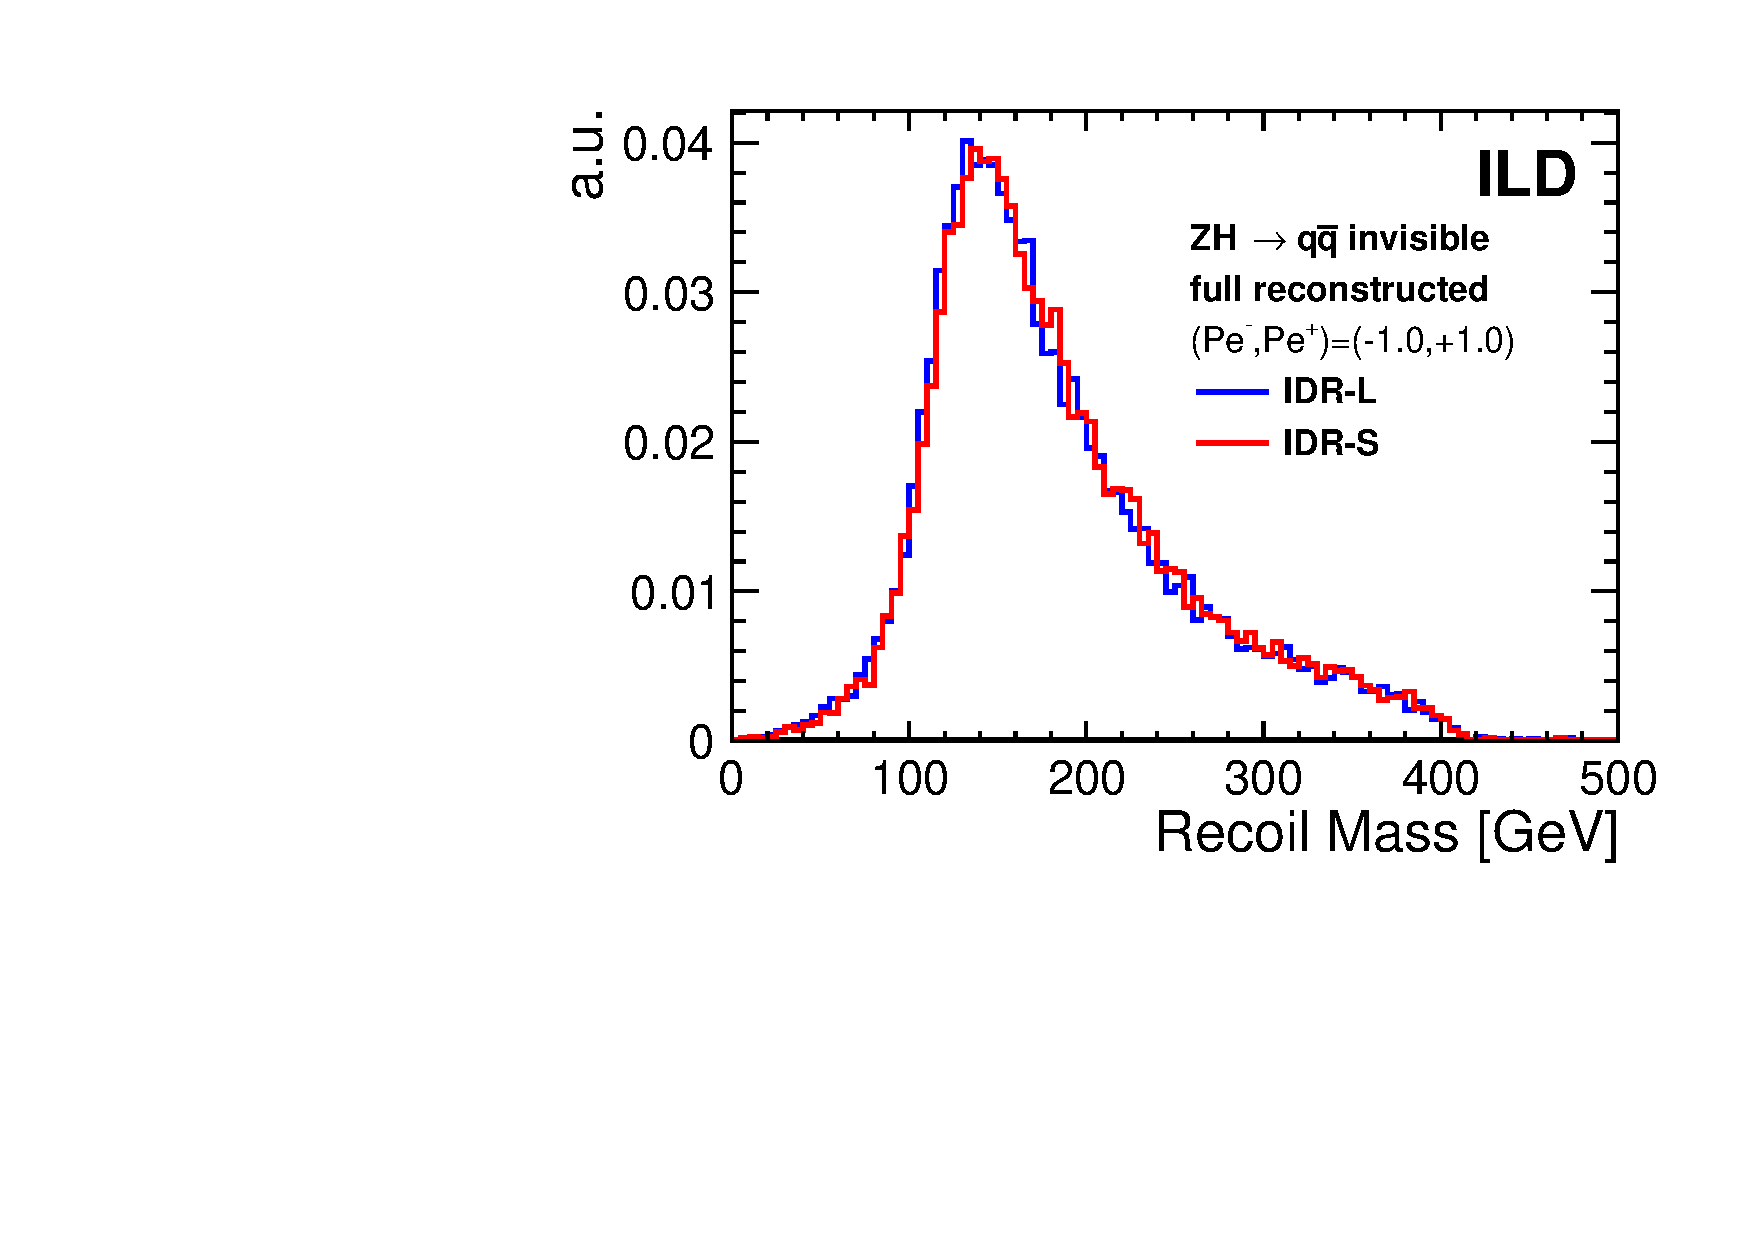
\includegraphics[width=\textwidth]{Performance/fig/compare_detector_mrec_lr.pdf}
 \caption{  \label{fig:Hinv:comp:mrec}}
 \end{subfigure}
%\end{center}
\caption{Comparison of the recoil mass distributions for IDR-L and IDR-S
(a) when cheating semi-leptonic decays, overlay removal, beam spectrum and ISR
(b) at full reconstruction level.
}
\label{fig:Hinv:comp}
\end{figure}

Figure~\ref{fig:Hinv:cheat:mjj} shows the di-jet invariant mass for the selected signal events at various levels of realism from the full reconstruction to cheating everything but the detector and particle flow performance. The first step of partial cheating removes jets with semileptonic heavy flavour decays. In a detector like ILD shower shapes in the highly-granular calorimeter and specific energy loss information from the TPC should allow an
excellent identification of leptons in jets, which, combined with secondary vertex information
should allow to significantly improve scale and resolution for heavy flavour jets with semileptonic decays. However, the corresponding reconstruction algorithms are still under development and thus could not be applied here. Similarly, work is ongoing to improve the
removal of overlay backgrounds, see e.g.\ Sec.~\ref{subsec:bench:higgsino} and Ref.~\cite{Boronat:2014hva}. Thus, we expect that with future reconstruction improvements, a performance similar to the case ``w/o sld and overlay'' could be reached. The beam spectrum (BS) by construction does not affect the invariant di-jet mass. ISR, on the contrary, can lead to photons in the detector. In this analysis, no attempt has been made to identify the corresponding particle flow objects. Therefore, also a large part of the effect of ISR on the di-jet mass should be recoverable with a more sophisticated analysis. 

The corresponding situation for the recoil mass is shown in Fig.~\ref{fig:Hinv:cheat:mrec}.
Here, ISR and BS have a large impact since they lead to a deviation of the actual initial state of the hard interaction from the naive assumption. Since this effect is dominated by photons from ISR and BS which escape undetected along the beam pipe, no attempt has been made to correct the kinematics of those events in which a photon is detected. See e.g.\ Sec.~\ref{subsec:bench:extraH} for an analysis where such a correction is applied. 

The recoil mass distributions obtained with the large and small detector model are compared in Fig.~\ref{fig:Hinv:comp}. Thereby, Fig.~\ref{fig:Hinv:comp:mrec} shows the situation at the current full reconstruction level, while Fig.~\ref{fig:Hinv:comp:cheatmrec} cheats the effect of semi-leptonic decays, overlay removal, beam spectrum and ISR. In both cases, the recoil  mass is slightly shifted to higher values in case of the small detector, due to differences 
in the calibration of the particle flow for the two models. In addition, the cheated recoil mass distribution is a bit wider for the small detector, as expected from its slightly worse
JER, c.f.\ Fig.~\ref{fig:perf:pfa_jer}.

\begin{figure}[htbp]
\begin{center}
 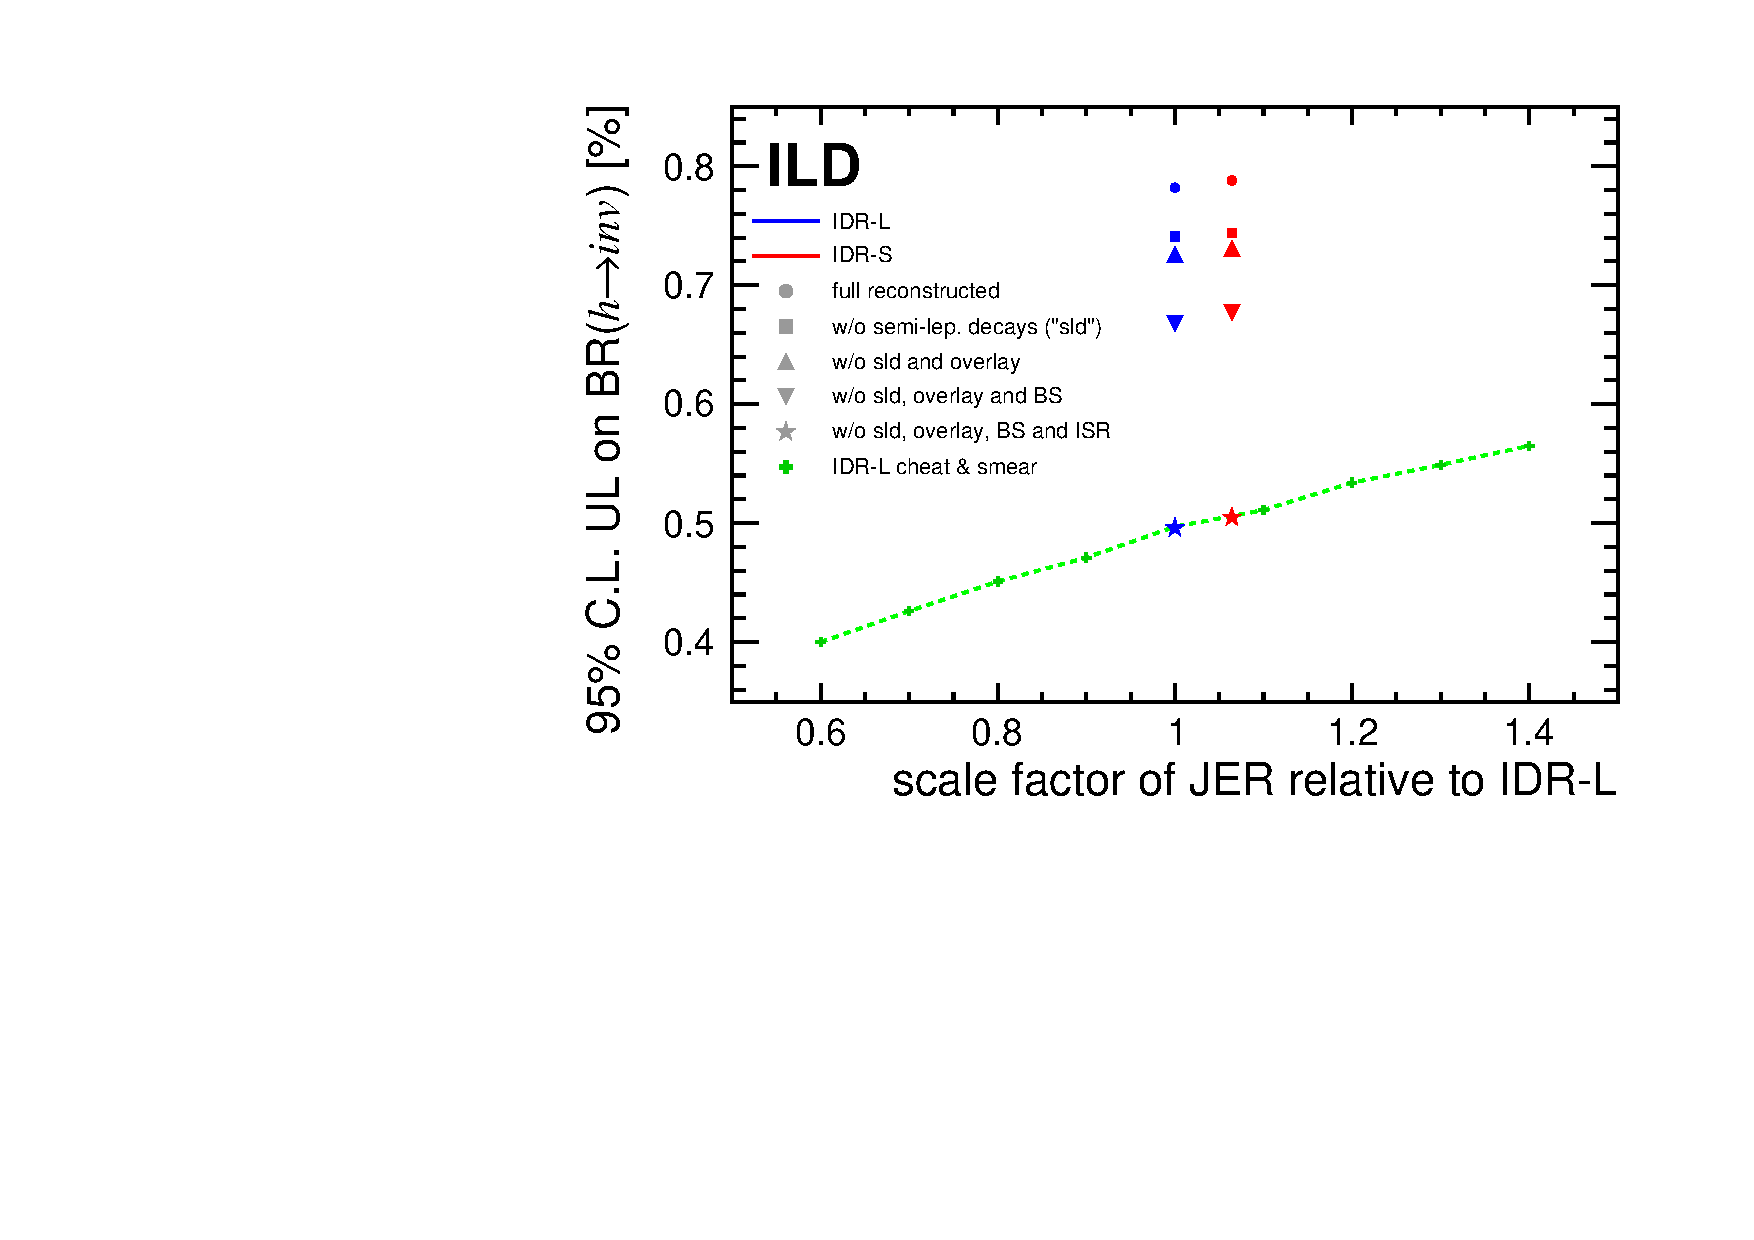
\includegraphics[width=0.75\textwidth]{Performance/fig/performance_plot.pdf}
\end{center}
\caption{Upper limit on $BR( \to $ invisible) at $95\%$ C.L. as a function of the jet energy resolution. The blue and red symbols show the results obtained from simulation of the IDR-L and IDR-S detector models, respectively, in full reconstruction and at various levels of cheating. The green crosses are obtained by varying the JER up and down w.r.t.\ IDR-L.
\fix{[JL: improve axis titles]}}
\label{fig:Hinv:BRlimit}
\end{figure}

The results in terms of the physics observable, namely the $95\%$ C.L.\ upper limit on $\sigma(q\bar{q} H)\times BR(H \to \mbox{inv.})$, are summarized in Fig.~\ref{fig:Hinv:BRlimit} for both detector models at the various cheating levels. In the case of full reconstruction, the upper limit is at 0.78\%  for IDR-L  and at  0.79\%  for IDR-S, corresponding to a relative change of about 1\%. At when isolating the effect of the particle flow performance by cheating all other aspects, the limit would be 0.50\% (0.51\%) for IDR-L (IDR-S), i.e.\ a relative change of about 2\%. Also displayed is an estimate of how
the cheated results would change when scaling the JER up and down. This clearly shows that
larger variations of the JER, by 20\% or so, have a clear impact on this physics analysis.
In the case of $\sqrt{s}=250$\,GeV, the impact of ISR and BS is much smaller, increasing the relative contribution from the JER.




%%%%%%%%%%%%%%%%%%%%%%%%%%%%%%%%%%%%%%%%%%%%%%%%%%%%%%%%%%%%%%%%%%%
%\subsection{\texorpdfstring{$\tau$}{Tau} decay modes and polarisation, \texorpdfstring{$A_{FB}$ and $A_{LR}$ in $e^+e^- \to \tau^+\tau^-$}{AFB and ALR in e+e- -> tau tau}}
\subsection{\texorpdfstring{$\tau$}{Tau} polarisation \texorpdfstring{in $e^+e^- \to \tau^+\tau^-$}{in e+e- -> tau tau}}
\fix{note in circulation!}

As shown in Sec.~\ref{sec:perf:hlr:tau}, the smaller ECAL inner radius of the small detector model slightly reduces the ability to identify the correct number of photons in
highly-boosted $\tau$ decays. Using the product of efficiency times purity as a figure of merit, this leads to a $5\%$ worse identification of $\tau \to \pi \nu$ and $\tau \to \rho \nu$ decays, while the identification of $\tau \to a_1 \nu$ decays deteriorates by about $15\%$ relative, c.f.\ Fig.~\ref{fig:HLR-tauID}. 

In order to evaluate the impact of this difference in a physics example, the measurement of the $\tau$ polarisation in $e^+e^- \to \tau^+\tau^-$ has been studied, looking specifically at events with no significant ISR, so those {\em not} returnin to the $Z$ pole. For the $\tau \to \pi \nu$ channels, the magnitude of the $\pi^{\pm}$ momentum can directly be used to extract the polarisation. In case of the $\tau \to \rho \nu$ decay, a polarimeter vector is constructed from the momenta of the $\pi^{\pm}$ and the $\pi^0$. A detailed description of the analysis and the polarisation extraction can be found in~\cite{ILDNote:tautau}.

\begin{figure}[htbp]
\begin{center}
 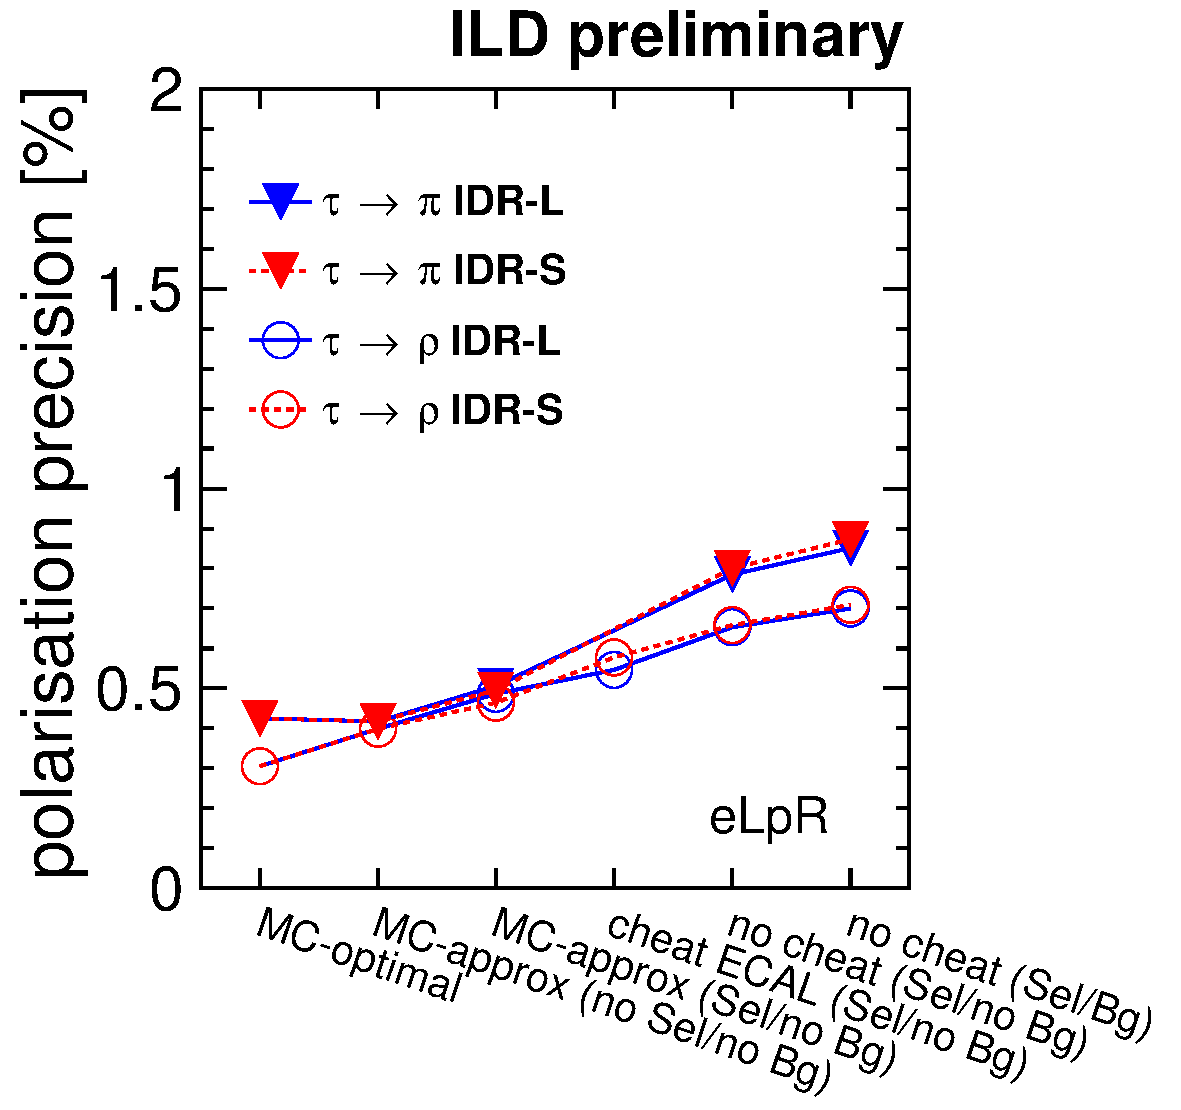
\includegraphics[width=0.55\textwidth]{Performance/fig/drawpexpresults0-update.pdf}
\end{center}
\caption{Precision on the $\tau$ polarisation achieved with IDR-L and IDR-S at various levels of cheating (see text) based on the $\pi$ and $\rho$ channels in the $P(e^-,e^+)=(-80\%,+30\%)$ data set.}
\label{fig:tautau:taupol}
\end{figure}

Figure~\ref{fig:tautau:taupol} illustrates the precision on the $\tau$ polarisation achieved with IDR-L and IDR-S  based on the $\pi$ and $\rho$ channels in the $P(e^-,e^+)=(-80\%,+30\%)$ data set, which dominates the combined precision. Thereby, various
levels of cheating are shown, starting from the optimal result when using all MC information, including the neutrino momentum. The next entry shows by how much the performance in the $\rho$ channel degrades by the approximate definition of the polarimeters used here\footnote{In principle, improved methods can be used, which however need further investigation~\cite{ILDNote:tautau}.}, followed by the application of the selection efficiency. The last three steps use the fully simulated and reconstructed events, apart from the entry ``cheat ECAL'', which uses MC information for the $\pi^0$ in the $\rho$ channel. In the last step, the full SM background is added. For the $\pi$-channel, the most significant effect occurs when reducing the number of signal events according to the selection efficiency of about $55\%$ observed in the full analysis. In case of the $\rho$-channel, all step contribute at a similar level to the final result. Overall, the differences between IDR-L and IDR-S are very small,  and probably due to limited MC statistics. 
%The largest deterioration of the precision occurs when applying the selection efficiency. Thus, future improvements of the di-$\tau$ selection have the largest potential for improving this measurement.

% \begin{figure}[htbp]
% %\begin{center}
% \begin{subfigure}{0.49\hsize} 
% %\includegraphics[width=\textwidth]{Performance/fig/}
%  \caption{ \label{fig:}}
%  \end{subfigure}
% %\hspace{0.03\textwidth}
% \begin{subfigure}{0.49\hsize} 
% %\includegraphics[width=\textwidth]{Performance/fig/}
%  \caption{  \label{fig:}}
%  \end{subfigure}
% %\end{center}
% \caption{
% (a) 
% (b) 
% }
% \label{fig:}
% \end{figure}

%%%%%%%%%%%%%%%%%%%%%%%%%%%%%%%%%%%%%%%%%%%%%%%%%%%%%%%%%%%%%%%%%%%
%\subsection{\texorpdfstring{$W$}{W} mass, Triple Gauge Couplings and Beam Polarisation from \texorpdfstring{$e^+e^- \to WW \to qql\nu$}{e+e- -> WW -> qqln}}
%%%%%%%%%%%%%%%%%%%%%%%%%%%%%%%%%%%%%%%%%%%%%%%%%%%%%%%%%%%%%%%%%%%
\subsection{Hadronic \texorpdfstring{$WW$ and $ZZ$}{WW and ZZ} separation in Vector Boson Scattering} 
\fix{everything done!} 

Vector boson scattering is an important process for testing the unitarisation of $WW$ scattering by the Higgs boson, as well as for measuring quartic gauge couplings, and thereby probing for anomalous contributions. Among all relevant final states, the reaction $e^+e^- \to \nu\nu VV \to \nu\nu qqqq$, where $VV$ can be $WW$ or $ZZ$, poses a particular challenge to the detectors and reconstruction algorithms, since it requires the separation of the hadronic $W$ and $Z$ decays without the ability to exploit kinematic constraints e.g.\ on the
total event energy due to the two invisible neutrinos.

This benchmark, at a center-of-mass energy of 1\,TeV, has already been studied in full detector simulation for the ILD LoI~\cite{ild:bib:ILDloi}. Now, we include for the first time all relevant aspects, in particular the full overlay from $\gamma\gamma \to$ low-$p_t$ hadrons and from $e^+e^-$ pair background, and we consider all quark flavours in the final state~\cite{ILDNote:QGCs}. The $W$ and $Z$ mass distributions obtained with the current full reconstruction are shown in Fig.~\ref{fig:qgc:rec}. Therein Fig.~\ref{fig:qgc:rec:1d} shows the average di-jet mass per event, comparing ILD-L and ILD-S, while Fig.~\ref{fig:qgc:rec:2d} shows the 2-dimensional distribution in the mass plane of the two invariant di-jet masses for ILD-L. At this level, no significant difference between the detector models can be observed.


%\thisfloatsetup{floatwidth=\SfigwFull,capposition=below}
\begin{figure}[htbp]
%\begin{center}
\begin{subfigure}{0.455\hsize} \includegraphics[width=\textwidth]{Performance/fig/ls_comp_rec_monly.pdf}
 \caption{ \label{fig:qgc:rec:1d}}
 \end{subfigure}
%\hspace{0.03\textwidth}
\begin{subfigure}{0.49\hsize} \includegraphics[width=\textwidth]{Performance/fig/m_m_rec.pdf}
 \caption{  \label{fig:qgc:rec:2d}}
 \end{subfigure}
%\end{center}
\caption{Dijet masses in $e^+e^- \to \nu\nu WW$ (blue) and $e^+e^- \to \nu\nu ZZ$ (red) events as obtained from the current full reconstruction.\\
(a) Average of the two di-jet masses per event.
(b) 2D illustration of the two di-jet masses per event.
}
\label{fig:qgc:rec}
\end{figure}


\begin{figure}[htbp]
%\begin{center}
\begin{subfigure}{0.475\hsize} \includegraphics[width=\textwidth]{Performance/fig/ls_comp_icn_noSLD_monly.pdf}
 \caption{ \label{fig:qgc:cheat:1d}}
 \end{subfigure}
%\hspace{0.03\textwidth}
\begin{subfigure}{0.49\hsize} \includegraphics[width=\textwidth]{Performance/fig/m_m_icn_noSLD.pdf}
 \caption{  \label{fig:qgc:cheat:2d}}
 \end{subfigure}
%\end{center}
\caption{Dijet masses in $e^+e^- \to \nu\nu WW$ (blue) and $e^+e^- \to \nu\nu ZZ$ (red) events as obtained when cheating the jet clustering and excluding events where one (or more) jets contain semi-leptonic charm or beauty decays.\\ 
(a) Average of the two di-jet masses per event. 
(b) 2D illustration of the two di-jet masses per event.
}
\label{fig:qgc:cheat}
\end{figure}


\begin{figure}[htbp]
\begin{center}
\begin{subfigure}{0.495\hsize} \includegraphics[width=\textwidth]{Performance/fig/l_WW_cheating_steps.pdf}
 \caption{ \label{fig:qgc:cheat:WW}}
 \end{subfigure}
%\hspace{0.03\textwidth}
\begin{subfigure}{0.495\hsize} \includegraphics[width=\textwidth]{Performance/fig/l_ZZ_cheating_steps.pdf}
 \caption{  \label{fig:qgc:cheat:ZZ}}
 \end{subfigure}
%\end{center}
\begin{subfigure}{0.495\hsize} \includegraphics[width=\textwidth]{Performance/fig/l_WW_cheating_steps_highQ2.pdf}
 \caption{ \label{fig:qgc:cheat:WWQ2}}
 \end{subfigure}
%\hspace{0.03\textwidth}
\begin{subfigure}{0.495\hsize} \includegraphics[width=\textwidth]{Performance/fig/l_ZZ_cheating_steps_highQ2.pdf}
 \caption{  \label{fig:qgc:cheat:ZZQ2}}
 \end{subfigure}
\end{center}
\caption{Average di-jet masses as obtained in full reconstruction at various levels of cheating.\\
(a) inclusive $e^+e^- \to \nu\nu WW$ events. 
(b) inclusive $e^+e^- \to \nu\nu ZZ$ events.
(c)  $e^+e^- \to \nu\nu WW$ events with $M(WW)>500$\,GeV. 
(d)  $e^+e^- \to \nu\nu ZZ$ events with $M(ZZ)>500$\,GeV.
}
\label{fig:qgc:cheatWWZZ}
\end{figure}

Figure~\ref{fig:qgc:cheat} shows the analogous distributions obtained when cheating the jet clustering (incl.\ the overlay removal), the jet pairing and when excluding events with semi-leptonic decays of heavy quarks, so that only the effects of the natural widths of the bosons, of fragmentation and hadronisation as well as the JER itself remain. Also here, no striking difference between the models can be seen, which leads to the conclusion that on this event sample, which is dominated by events with rather low invariant masses of the di-boson system, the effect of the slightly worse JER of ILD-S is hidden beneath the width and fragmentation/hadronisation corrections.


Nevertheless, the differences between Fig.~\ref{fig:qgc:rec} and Fig.~\ref{fig:qgc:cheat} are striking. Therefore, we investigated the impact of the size of various contributions individually as shown in Fig.~\ref{fig:qgc:cheatWWZZ}, for ILD-L only. For the inclusive $WW$ and $ZZ$ samples, shown in Figs.~\ref{fig:qgc:cheat:WW} and~\ref{fig:qgc:cheat:ZZ}, the dominant effect is the residual of the non-perfect overlay removal, followed by the jet clustering itself and the semi-leptonic decays. Non-perfect jet pairing only plays a minor role. This can be compared to the situation found when only considering events with high $WW$/$ZZ$ invariant masses, shown in Figs.~\ref{fig:qgc:cheat:WWQ2} and~\ref{fig:qgc:cheat:ZZQ2}. In this case, the impact of non-perfect jet clustering is reduced to a negligible level. Instead, the effect of the residual overlay from low-$p_t$ $\gamma \gamma \to $hadron events dominates. For the $ZZ$ events, also the missing neutrinos from semi-leptonic heavy quark decays play a visible role. 
These results demonstrate the need for development of more sophisticated high-level reconstruction algorithms, in particular for the overlay removal, the jet clustering and the identification and correction of semi-leptonic heavy flavour decays. For all these cases promising tools are under development, see e.g.\ Sec.~\ref{subsec:bench:higgsino} and Ref.~\cite{Boronat:2014hva}.

%%%%%%%%%%%%%%%%%%%%%%%%%%%%%%%%%%%%%%%%%%%%%%%%%%%%%%%%%%%%%%%%%%%
\subsection{Photon Energy Scale Calibration from \texorpdfstring{$e^+e^- \to \gamma Z \to \gamma \mu^+\mu^-$}{e+e- -> aZ -> mumu}}
\label{subsec:bench:gammaZ}
%%%%%%%%%%%%%%%%%%%%%%%%%%%%%%%%%%%%%%%%%%%%%%%%%%%%%%%%%%%%%%%%%%%
\fix{IDR draft signed off by Matthew (referee) and Takahiro. Note in a very incomplete state.}

Di-fermion production, with or without radiative return to the $Z$ pole, is an integral part of the ILC physics case. In addition, the radiative return events offer an important
opportunity to cross calibrate the energy scales of various subdetectors. As a detector benchmark, we chose here the example of calibrating the photon energy scale against the momentum scale of the tracker. Thereby, the momenta and angles of the muons as well as the 
polar and aziumuthal angle of the photon serve as input, from which the energy of the photon and the amount of energy lost in beamstrahlung and collinear ISR are determined by
requiring conservation of energy and $p_y$ between initial and final state. It should be stressed that it is not necessary to apply a $Z$ mass constraint, which would introduce an additional uncertainty due to the large natural width of the $Z$ resonance. A full description of this and alternative methods can be found in~\cite{ILDNote:gammaZ}.
 

\begin{figure}[htbp]
\begin{subfigure}{0.49\hsize} 
 \includegraphics[width=\textwidth]{Performance/fig/IDR1MethodComp.pdf}
 \caption{ \label{fig:gammaZ:meanE:allE}}
 \end{subfigure}
\begin{subfigure}{0.49\hsize} 
 \includegraphics[width=\textwidth]{Performance/fig/IDR5ECentervalueE.pdf}
 \caption{  \label{fig:gammaZ:meanE:vsE}}
 \end{subfigure}
\caption{
Deviation of the photon energy from its true value when using non-perfectly calibrated PFO-level energies (cyan), when calculating the photon energy from the $\mu$ momenta and kinematic constraints (blue, ``angular method'') and after calibrating the mean PFO-level w.r.t.\ the mean obtained from the $\mu$ momenta (green).  
(a) Distribution of deviation for all photons in the sample.
(b) Mean deviation in bins of the photon energy.
}
\label{fig:gammaZ:meanE}
\end{figure}

Figure~\ref{fig:gammaZ:meanE} illustrates the power of this method by application to a non-perfectly calibrated photon reconstruction in the large detector model, both inclusively for all photons (Fig.~\ref{fig:gammaZ:meanE:allE}) and in bins of the photon energy (Fig.~\ref{fig:gammaZ:meanE:vsE}). Since the $e^+e^- \to \mu^+\mu^-\gamma$ sample
is dominated by radiative returns to the $Z$ pole, the majority of photons has high energies close to $241$\,GeV.

\begin{figure}[htbp]
\begin{subfigure}{0.49\hsize} 
 \includegraphics[width=\textwidth]{Performance/fig/IDR4EResolutionE.pdf}
 \caption{ \label{fig:gammaZ:sigmaE:rel}}
 \end{subfigure}
\begin{subfigure}{0.49\hsize} 
 \includegraphics[width=\textwidth]{Performance/fig/IDR6EScaleUncertainty.pdf}
 \caption{  \label{fig:gammaZ:sigmaE:abs}}
 \end{subfigure}
\caption{Uncertainty on the photon energy scale calibration as a function of the photon energy for IDR-L and IDR-S.
(a) Relative uncertainty when using non-perfectly calibrated PFO-level energies (cyan/magenta) and when calculating the photon energy from the $\mu$ momenta and kinematic constraints (blue/red, ``angular method'').
(b) Absolute uncertainty from the angular method in MeV.
}
\label{fig:gammaZ:sigmaE}
\end{figure}

\begin{figure}[htbp]
\begin{subfigure}{0.49\hsize} 
 \includegraphics[width=\textwidth]{Performance/fig/IDR2EResolutionTheta.pdf}
 \caption{ \label{fig:gammaZ:angles:theta}}
 \end{subfigure}
\begin{subfigure}{0.49\hsize} 
 \includegraphics[width=\textwidth]{Performance/fig/IDR3EResolutionPhi.pdf}
 \caption{  \label{fig:gammaZ:angles:phi}}
 \end{subfigure}
\caption{
Resolution of the photon energy when using non-perfectly calibrated PFO-level energies (cyan/magenta) and when calculating the photon energy from the $\mu$ momenta and kinematic constraints (blue/red, ``angular method'').  
(a) as a function of the polar angle
(b) as a function of the azimuthal angle
}
\label{fig:gammaZ:angles}
\end{figure}

The resolution of angular method, i.e.\ the width of the blue distribution in Fig.~\ref{fig:gammaZ:meanE:allE} is shown for IDR-L and IDR-R in Fig.~\ref{fig:gammaZ:sigmaE:rel} as a function of the photon energy. This translates into
an absolute uncertainty on the photon energy scale calibration of about $10$\,MeV for high-energy photons, as shown in Fig.~\ref{fig:gammaZ:sigmaE:abs}. 
The angular dependencies of the resolution of this method are shown in Fig.~\ref{fig:gammaZ:angles}. As a function of the polar angle, Fig.~\ref{fig:gammaZ:angles:theta} clearly shows the effect of the better momentum resolution of IDR-L for central high-momentum tracks, while in the two most forward bins, the small detector performs better due to its higher magnetic field. As a function of the azimuthal angle, there is no particular region where the performance of the two detector models differs, as can be seen in Fig.~\ref{fig:gammaZ:angles:phi}. The modulation of the resolution with $\phi$ is an effect of using the $p_y$ constraint only, which is the easiest method as the $p_y$ conservation is not influenced by the beam crossing angle. The modulation will be reduced when also $p_x$ balance is exploited e.g.\ in a kinematic fit.

%%%%%%%%%%%%%%%%%%%%%%%%%%%%%%%%%%%%%%%%%%%%%%%%%%%%%%%%%%%%%%%%%%%
\subsection{\texorpdfstring{$A_{FB}$ and polarised cross sections from $e^+e^- \to b\bar{b}$}{AFB and ALR from ee -> bb}}
\label{subsec:bench:bbbar}
%%%%%%%%%%%%%%%%%%%%%%%%%%%%%%%%%%%%%%%%%%%%%%%%%%%%%%%%%%%%%%%%%%%
\fix{approved by Roman, joint note with $e^+e^- \to t\bar{t}$ very close to final}

The measurement of the polar angle spectrum and hence of the forward backward asymmetries of $b$-quarks requires to distinguish the jet from the $b$-quark from the $\bar{b}$-jet. The two most important techniques for this are the reconstruction of the charge at the secondary vertex, and the identification of charged Kaons in the $b$-decay chain. While the first method requires a complete reconstruction of all tracks from the secondary vertices, the Kaon ID hinges upon a special
feature of ILD, namely the measurement of the specific energy loss $dE/dx$ in the TPC. In order to arrive at a reliable $b$-charge measurement, a consistent double-tag is required for each event, allowing for all four  possible combinations of the two techniques. All details of the event reconstruction and selection can be found in~\cite{ILDNote:bbtt}.

\begin{figure}[htbp]
%\begin{center}
\begin{subfigure}{0.49\hsize} 
\includegraphics[width=\textwidth]{Performance/fig/acceptance_2models_v2.pdf}
 \caption{ \label{fig:bbbar:effipur:effi}}
 \end{subfigure}
%\hspace{0.03\textwidth}
\begin{subfigure}{0.49\hsize} 
\includegraphics[width=\textwidth]{Performance/fig/purity_v2.pdf}
 \caption{  \label{fig:bbbar:effipur:pur}}
 \end{subfigure}
%\end{center}
\caption{
(a) Acceptance of the $e^+e^- \to b\bar{b}$ analysis as a function of $\cos{\theta}$ of the $b$-quark for IDR-L and IDR-S.
(b) Purity of the four different categories for charge tagging for IDR-L and IDR-S. 
}
\label{fig:bbbar:effipur}
\end{figure}

Figure~\ref{fig:bbbar:effipur:effi} compares the acceptance of the $b$-jet reconstruction for the large and the small version of ILD.
For $|\cos{\theta_b}|<0.5$, corresponding to a large part of the endcap 
region, the acceptance of IDR-L if about 1\% larger than for IDR-L. The purity of the four combinations of charge-ID (two methods times two jets) is shown in Fig.~\ref{fig:bbbar:effipur:pur}. While the charge-ID via vertex charge performs identically for both detectors, the Kaon-charge ID yields a higher purity for IDR-L due to the larger radius of the TPC, which improves the $dE/dx$ resolution. 

The reconstructed  $|\cos{\theta_b}|$ distribution is shown in Fig.~\ref{fig:bbbar:result} for an integrated luminosity of $46$\,fb$^{-1}$ with purely left-handed electrons and right-handed positrons. The distributions obtained for both detectors are compared with the parton level. The results for both detector models agree within the statistical uncertainty corresponsind to the size of the simulated sample. However there seems to be a larger migration in case of the small detector model.


\begin{figure}[htbp]
\begin{center} \includegraphics[width=0.55\textwidth]{Performance/fig/result2models_v3.pdf}
\end{center}
\caption{Generator-level distribution of $\cos{\theta_b}$ and the corresponding reconstructed distributions for IDR-L and IDR-S. The distribution is shown for a simulated sample of $46$\,fb$^{-1}$ for pure $e^-_L e^+_R$ beams.}
\label{fig:bbbar:result}
\end{figure}

%%%%%%%%%%%%%%%%%%%%%%%%%%%%%%%%%%%%%%%%%%%%%%%%%%%%%%%%%%%%%%%%%%%
\subsection{\texorpdfstring{$A_{FB}$ and polarised cross sections from $tt \to bb qql\nu$}{AFB and ALR from tt -> bbqqlv}}
\label{subsec:bench:ttbar}
%%%%%%%%%%%%%%%%%%%%%%%%%%%%%%%%%%%%%%%%%%%%%%%%%%%%%%%%%%%%%%%%%%%
\fix{approved by Roman, joint note with $e^+e^- \to b\bar{b}$ very close to final}

The forward-backward asymmetry and the polarised cross sections of $e^+e^- \to t\bar{t}$ are crucial ingredients to the determination of the couplings of top quark to the photon and the $Z$ boson. 
As a benchmark, the semi-leptonic channel, which represents 43.5\% of all $t \bar t$ decays has been studied~\cite{ILDNote:bbtt}. In the semi-leptonic decay channel the lepton charge is available to distiguish between the $t$ and the $\bar{t}$ quark. In the fully hadronic case, representing 46.5\% of all $t\bar t$ decays, only vertex and and kaon charge is available. It is therefore instructive to study and add events in which also vertex charge and Kaon-ID information have been used, based on the analysis techniques employed for the $e^+e^- \to b\bar{b}$ benchmark described in the previous section.

The purities of several double-tag combinations are compared for the large and small detector models in Fig.~\ref{fig:ttbar:effi}. While the size of the detector has no direct influence on the semi-leptonic analysis, especially the Kaon-ID based methods achieve a higher purity in case of the large detector. 


\begin{figure}[htbp]
\begin{center} \includegraphics[width=0.55\textwidth]{Performance/fig/p_value_l5_ele_mu_noLcut-v1.pdf}
\end{center}
\caption{Purity of various methods to identify the charge of the $t$/$\bar{t}$ quarks.}
\label{fig:ttbar:effi}
\end{figure}

\begin{figure}[htbp]
%\begin{center}
\begin{subfigure}{0.475\hsize} 
\includegraphics[width=\textwidth]{Performance/fig/compare_normalized_b.pdf}
 \caption{ \label{fig:ttbar:costhetab}}
 \end{subfigure}
%\hspace{0.03\textwidth}
\begin{subfigure}{0.475\hsize} 
\includegraphics[width=\textwidth]{Performance/fig/compare_normalized.pdf}
 \caption{  \label{fig:ttbar:costhetat}}
 \end{subfigure}
%\end{center}
\caption{Generator-level polar angle distributions and the corresponding reconstructed distributions for IDR-L and IDR-S. The distributions are shown for pure $e^-_L e^+_R$ data.
(a) Polar angle of the $b$-quark $\cos{\theta_b}$. 
(b) Polar angle of the $t$-quark $\cos{\theta_t}$.
}
\label{fig:ttbar:result}
\end{figure}

The reconstructed  polar angle ($\cos{\theta_t}$) distribution is shown for the purely left-handed electron and purely right-handed positron case in Fig.~\ref{fig:ttbar:costhetat}. Figure~\ref{fig:ttbar:costhetab} shows the polar angle spectrum of the $b$ quark that is emitted from the $t$ decay. This observable has been studied for the first time for the IDR and adds to the physics potential of ILD.  Both, the polar angle spectrum of the $t$ quark and of the $b$ quark, have been compared to the parton level for the two detector models under study. No difference is found here between the two detector models.
 
\begin{figure}[htbp]
%\begin{center}
\begin{subfigure}{0.475\hsize} 
\includegraphics[width=\textwidth]{Performance/fig/b_1-modif.png}
 \caption{ \label{fig:ttbar:costhetabRL}}
 \end{subfigure}
%\hspace{0.03\textwidth}
\begin{subfigure}{0.475\hsize} 
\includegraphics[width=\textwidth]{Performance/fig/t_1-modif.png}
 \caption{  \label{fig:ttbar:costhetatRL}}
 \end{subfigure}
%\end{center}
\caption{Generator-level polar angle distributions and the corresponding reconstructed distributions for IDR-L and IDR-S. The distributions are shown for pure $e^-_R e^+_L$ data.
(a) Polar angle of the $b$-quark $\cos{\theta_b}$. 
(b) Polar angle of the $t$-quark $\cos{\theta_t}$.
}
\label{fig:ttbar:resultRL}
\end{figure}

The analogous distributions are shown in Fig.~\ref{fig:ttbar:resultRL} for the opposite beam helicity configuration, again compared to the parton level. Also here, no difference is found here between the two detector models.  Note the difference in the polar angle spectra of the $b$ quark between Figs.~\ref{fig:ttbar:costhetab} and~\ref{fig:ttbar:costhetabRL} that are due to the $V-A$ interaction at the $tbW$ vertex.

The resulting precisions on the polarised cross sections as well as on $A_{FB}$ as expected for the $P(e^-,e^+)=(\pm 80\%, \mp 30\%)$ data sets are equal for the two detector models as given in Tab.~\ref{tab:AFBtt}.

\begin{table}[htb]
\begin{center}
\begin{tabular}{|c|c|c|c|}
\hline
 & $P(e^-,e^+)$ & $(\delta\sigma / \sigma)_{stat} [\%]$ & $(\delta A_{FB}^t / A_FB^t)_{stat} [\%]$ \\
\hline
\multirow{2}{*}{IDR-L/S} &  $(-80\%,+30\%)$ & 0.17 & 0.7 \\
                         &  $(+80\%,-30\%)$ & 0.25 & 0.53 \\
\hline
\end{tabular}
\end{center}
\caption{Statistical uncertainties on the polarised cross section and the top forward-backward asymmetry from the canonic ILC500 data sets as obtained in this analysis.}
\label{tab:AFBtt}   
\end{table}    

In order to put these results into perspective, these results are translated into $1\sigma$ precisions on the electromagnetic form factors of the top quark. They are displayed in Fig.~\ref{fig:ttbar:formfac} in comparison to the most recent projections for HL-LHC and estimates for FCCee~\cite{Janot:2015yza}. The projections for HL-LHC are derived from the {\em individual} constraints of EFT Wilson coefficients presented in Tab. C2.3 of Ref.~\cite{Durieux:2019rbz} (the most favorable scenario for HL-LHC). This figure clearly demonstrates the superiority of a linear $e^+e^-$ collider with polarised beams operated at an adequate center-of-mass energy.             
\begin{figure}[htbp]
\begin{center} \includegraphics[width=0.6\textwidth]{Performance/fig/couplall.pdf}
\end{center}
\caption{Expected precision on electromagnetic form factors of the top quark from this study compared to HL-LHC and FCCee.}
\label{fig:ttbar:formfac}
\end{figure}

%%%%%%%%%%%%%%%%%%%%%%%%%%%%%%%%%%%%%%%%%%%%%%%%%%%%%%%%%%%%%%%%%%%
\subsection{Search for extra Higgs Bosons in \texorpdfstring{$e^+e^- \to Zh$}{e+e- -> Zh}}
\label{subsec:bench:extraH}
%%%%%%%%%%%%%%%%%%%%%%%%%%%%%%%%%%%%%%%%%%%%%%%%%%%%%%%%%%%%%%%%%%%
\fix{Note to be finalized}

Searches for additional Higgs bosons or other new scalar particles are theoretical well-motivated and highly
complementary to the sensitivity of hadron colliders. Due to the SM-likeness of the $125$-GeV Higgs boson, 
additional Higgs bosons are expected to have a suppressed coupling to the $Z$ boson. Nevertheless, they can 
be searched for using the same recoil technique which is the basis of the decay-mode independent measurement
of the total Higgsstrahlungs cross section. While in principle all visible decay modes of the $Z$ boson can
be exploited in this search, $Z\to\mu^+\mu^-$ as the cleanest mode has been chosen as a benchmark here~\cite{ILDNote:extraH}.
The two most important detector performance aspects for this analysis are the momentum resolution for the two
muons and the ability to detect and identify ISR photons in the detector. The latter applies in particular for the lower Higgs masses, where $M_h + M_Z << \sqrt{s}$ and thus significant photon radiation occurs frequently.
If the photon is detected, then the event kinematics can be corrected accordingly, improving the separation of signal and background significantly.


\begin{figure}[htbp]
%\begin{center}
\begin{subfigure}{0.475\hsize} 
\includegraphics[width=\textwidth]{Performance/fig/lepton_pair_inm_difference_nh20.pdf}
 \caption{ \label{fig:extraH:Mdiff:mh20}}
 \end{subfigure}
%\hspace{0.03\textwidth}
\begin{subfigure}{0.475\hsize} 
\includegraphics[width=\textwidth]{Performance/fig/lepton_pair_inm_difference_nh100.pdf}
 \caption{  \label{fig:extraH:Mdiff:mh100}}
 \end{subfigure}
\begin{subfigure}{0.475\hsize} 
\includegraphics[width=\textwidth]{Performance/fig/lepton_pair_inm_difference_nh300.pdf}
 \caption{ \label{fig:extraH:Mdiff:mh300}}
 \end{subfigure}
%\hspace{0.03\textwidth}
\begin{subfigure}{0.475\hsize} 
\includegraphics[width=\textwidth]{Performance/fig/lepton_pair_inm_difference_2f.pdf}
 \caption{  \label{fig:extraH:Mdiff:2f}}
 \end{subfigure}
%\end{center}
\caption{Event-by-event difference between reconstructed and generated di-muon mass for different types of events sampling different ranges in polar angle and momentum of the muons  in IDR-L and IDR-S:
(a) $Zh$ signal with $M_h = 20$\,GeV
(b) $Zh$ signal with $M_h = 100$\,GeV
(c) $Zh$ signal with $M_h = 300$\,GeV
(d) $2f$ background.
}
\label{fig:extraH:Mdiff}
\end{figure}

Figure~\ref{fig:extraH:Mdiff} shows the event-by-event difference between the reconstructed and generated di-muon mass for signal events with different Higgs masses as well as for the 2-fermion background. Since the underlying distributions in momentum and polar angle differ significantly, also the difference between IDR-L and IDR-S varies between the different samples. With higher Higgs masses, the $Z$ is less and less boosted, thus the muons are more and more central and back-to-back, resulting in an overall better mass reconstruction and a better performance of the large detector. In case of the $2$-fermion background, about half of the events returns to the $Z$ pole, resulting in forward boosted $Z$'s with a small opening angle between the also forward-going muons. In those events which do not return to the $Z$, the muons have higher momenta than in the
signal samples. In combination, the mass reconstruction in the $2$-fermion events is worse, but when comparing
the two detector models, the better momentum resolution of ILD-S in the forward region and its worse resolution
in the barrel roughly cancel.




This can be seen much more clearly from the event-by-event mass resolution as calculated from the errors on 
the track parameters, shown in Fig~\ref{fig:extraH:Msigma} for the same four event samples. In case of the Higgs
signal, the large detector always gives a significantly better resolution. In case of the $2$-fermion background, there is a population at the best resolutions which behaves like the signal, while at the worse
resolutions the small detector performs better than the large.

\begin{figure}[htbp]
%\begin{center}
\begin{subfigure}{0.475\hsize} 
\includegraphics[width=\textwidth]{Performance/fig/lepton_pair_inm_sigma_nh20.pdf}
 \caption{ \label{fig:extraH:Msigma:mh20}}
 \end{subfigure}
%\hspace{0.03\textwidth}
\begin{subfigure}{0.475\hsize} 
\includegraphics[width=\textwidth]{Performance/fig/lepton_pair_inm_sigma_nh100.pdf}
 \caption{  \label{fig:extraH:Msigma:mh100}}
 \end{subfigure}
\begin{subfigure}{0.475\hsize} 
\includegraphics[width=\textwidth]{Performance/fig/lepton_pair_inm_sigma_nh300.pdf}
 \caption{ \label{fig:extraH:Msigma:mh300}}
 \end{subfigure}
%\hspace{0.03\textwidth}
\begin{subfigure}{0.475\hsize} 
\includegraphics[width=\textwidth]{Performance/fig/lepton_pair_inm_sigma_2f.pdf}
 \caption{  \label{fig:extraH:Msigma:2f}}
 \end{subfigure}
%\end{center}
\caption{Event-by-event mass resolution calculated by error propagation from the track fit for different types of events sampling different ranges in polar angle and momentum of the muons in IDR-L and IDR-S:
(a) $Zh$ signal with $M_h = 20$\,GeV
(b) $Zh$ signal with $M_h = 100$\,GeV
(c) $Zh$ signal with $M_h = 300$\,GeV
(d) $2f$ background.
}
\label{fig:extraH:Msigma}
\end{figure}

% Figure~\ref{fig:extraH:ISRTagging} compares the performance of IDR-L and IDR-S in terms of the identification of ISR photons. \fix{[JL: at which level of the analysis is this plot made, and with which algorithm? Need documentation in note...]}
% 
% \begin{figure}[htbp]
% \begin{center} 
% \includegraphics[width=0.55\textwidth]{Performance/fig/ISRphoton_tagging_efficiency.pdf}
% \end{center}
% \caption{Performance of the ISR photon identification in IDR-L and IDR-S. True ISR photons are considered as signal, while the background comprises all PFOs identified as ISR photon, but having another true origin. \fix{[JL: improve plot layout]}}
% \label{fig:extraH:ISRTagging}
% \end{figure}

Figure~\ref{fig:extraH:limit} shows the resulting $95\%$ CL sensitivity on the mixing of the new scalar with the SM-like Higgs boson, $\sin^2{\theta}$, as a function of the scalar mass $M_{S^0}$. Also shown is the corresponding observed limit by the OPAL collaboration~\cite{Abbiendi:2002qp}. Note that for scalar masses below about $140$\,GeV, the ILC run at $\sqrt{s}=250$\,GeV probes significantly smaller mixing angles $\sin^2{\theta}$. So significant difference between IDR-L and IDR-S is observed at this level. At low $M_{S^0}$, the current results are, however, limits by the avaible SM background MC statistics. In the corresponding analysis at $\sqrt{s}=250$\,GeV it has been observed that the detector performance matters most for $M_{S^0}<80$\,GeV, dominated by the ability to reconstruct and identify ISR photons~\cite{FIPnote:ESU_BSM}.

\begin{figure}[htbp]
\begin{center} 
\includegraphics[width=0.55\textwidth]{Performance/fig/exclusion_limits_compare_LEP.pdf}
\end{center}
\caption{Expected sensitivity at the $95\%$ CL for IDR-L and IDR-S compared to the existing limit from LEP~\cite{Abbiendi:2002qp}. Note that for scalar masses below about $140$\,GeV, the ILC run at $\sqrt{s}=250$\,GeV probes significantly smaller mixing angles $\sin^2{\theta}$~\cite{FIPnote:ESU_BSM}.}
\label{fig:extraH:limit}
\end{figure}



%%%%%%%%%%%%%%%%%%%%%%%%%%%%%%%%%%%%%%%%%%%%%%%%%%%%%%%%%%%%%%%%%%%
\subsection{Search for low \texorpdfstring{$\Delta M$}{DeltaM} Higgsinos}
\label{subsec:bench:higgsino}
%%%%%%%%%%%%%%%%%%%%%%%%%%%%%%%%%%%%%%%%%%%%%%%%%%%%%%%%%%%%%%%%%%%
\fix{physics performance still w.i.p. - time scale somewhat unclear...}

New particles with maximally electroweak interactions and small mass differences in the decay chain are among the prime examples of discovery opportunities at future $e^+e^-$ colliders. A famous example of such kind of
new physics are higgsinos, which are expected to be light in natural SUSY models and tend to have small mass
splittings, in particular when the gaugino masses are much heavier. One of the model points studied previously in fast detector simulation~\cite{Berggren:2013vfa}, with a mass splitting of only $770$\,MeV between the chargino and the LSP, is used as a detector performance benchmark here~\cite{ILDNote:higgsinos}. The mass of the
chargino is about 167\,GeV.

Figure~\ref{fig:higgsino:trkeffi} shows the tracking efficiency as a function of transverse momentum as obtained
in these events at a center-of-mass energy of $500$\,GeV. For transverse
momenta below $p_t = 300$\,MeV, a clear difference can be seen between the two detector models due to the higher magnetic field of IDR-S. For this specific model point, which lies -- with $2 M(\tilde{\chi}^{\pm}_1) \approx 330$\,GeV -- significantly below the kinematic limit, the efficiency to detect all charged decay products is around $60$\% and differs only by $2$\% between IDR-L and IDR-S, thanks to the sufficient boost of the charginos. For chargino masses closer to the kinematic limit, however, the typical $p_t$ will be even lower, 
and the difference visible in Fig~\ref{fig:higgsino:trkeffi} will lead to a larger effect.
The low $p_t$ tracking efficiency could be recovered at least partially by reducing the radii of the vertex detector layers for IDR-S, which is possible since the higher magnetic field also confines the pair background at smaller radii.
\begin{figure}[htbp]
\begin{center}
 \includegraphics[width=0.6\textwidth]{Performance/fig/Tracking_efficiency.pdf}
\end{center}
\caption{Tracking efficiency obtained in IDR-L and IDR-S for pair production of charginos which are only $770$\,MeV more heavy than the LSP and thus have only very few and soft visible decay products.
}
\label{fig:higgsino:trkeffi}
\end{figure}


%%%%%%%%%%%%%%%%%%%%%%%%%%%%%%%%%%%%%%%%%%%%%%%%%%%%%%%%%%%%%%%%%%%
\subsection{WIMP Search in the Mono-Photon Channel}

\fix{note to be finalized}
%%%%%%%%%%%%%%%%%%%%%%%%%%%%%%%%%%%%%%%%%%%%%%%%%%%%%%%%%%%%%%%%%%%
The search for WIMP production via the mono-photon signature is another example of a search highly complementary to the HL-LHC, which predominantly probes couplings of WIMPs to quarks. This channel has been chosen as a  benchmark specifically in order to test the photon reconstruction and the performance of the BeamCal, which plays an essential role in vetoing background from Bhabha scattering. The benchmark analysis is described in more detail in~\cite{ILDNote:WIMPs} and closely follows~\cite{Habermehl:2018yul}.
\begin{figure}[htbp]
%\begin{center}
\begin{subfigure}{0.49\hsize} 
\includegraphics[width=\textwidth]{Performance/fig/NrecNgenE_photon_IDR_wo_cosTheta08.pdf}
 \caption{ \label{fig:WIMP:Ngamma:Egood}}
 \end{subfigure}
%\hspace{0.03\textwidth}
\begin{subfigure}{0.49\hsize} 
\includegraphics[width=\textwidth]{Performance/fig/NrecNgenCosTheta_allpfo_IDR.pdf}
 \caption{  \label{fig:WIMP:NPFO:theta}}
 \end{subfigure}
% \begin{subfigure}{0.49\hsize} 
% \includegraphics[width=\textwidth]{Performance/fig/NrecNgenE_photon_IDR.pdf}
%  \caption{ \label{fig:WIMP:Ngamma:E}}
%  \end{subfigure}
% %\hspace{0.03\textwidth}
% \begin{subfigure}{0.49\hsize} 
% \includegraphics[width=\textwidth]{Performance/fig/NrecNgenCosTheta_photon_IDR.pdf}
%  \caption{  \label{fig:WIMP:Ngamma:theta}}
%  \end{subfigure}
%\end{center}
\caption{Ratio of recontructed and generated PFOs per event 
(a) based on PFOs identified as photons as function of the photon energy, excluding the corner region between barrel and endcap ($|\cos{\theta}|\simeq 0.8$)
(b) based all PFOs as function of the photon polar angle.}

%(c) based on PFOs identified as photons as function of the photon energy
%(d) based PFOs identified as photons as function of the photon polar angle. 
%}
\label{fig:WIMP:Ngamma}
\end{figure}

Figure~\ref{fig:WIMP:Ngamma} shows the ratio of recontructed and generated photons per event as a function of
the photon's energy and polar angle. While it has been shown in~\cite{Habermehl:2018yul} that the actual energy
resolution is not very critical in this analysis, it is important that the number of photons is correct, since the signature of a single photon and no other significant detector activity forms the basis of the selection.
As can be seen in Fig.~\ref{fig:WIMP:Ngamma:Egood}, the average number of reconstructed photons per generated photon tends to be a few permille below 1 at low photon energies. With increasing photon energy, the tendency of the particle flow reconstruction to split a photon into two increases, but stays below the level of 1\% for IDR-L and below 2\% for IDR-S. In both cases, the corner region between barrel and endcap has been excluded, because the current reconstruction software tends to split PFOs in this region. This can be clearly seen in 
Fig.~\ref{fig:WIMP:NPFO:theta} which shows the ratio of reconstructed PFOs vs generated particles as a function of $\cos{\theta}$. Also indicated are the locations of the barrel-endcap transition for IDR-L and IDR-S, which occurs at different  due to the different $\cos{\theta}$ values due to the different aspect ratios of the two detector models.  All the features in these two plots are expected to be reducable with further development of the particle flow reconstruction.

\begin{figure}[htbp]
%\begin{center}
\begin{subfigure}{0.49\hsize} 
%\includegraphics[width=\textwidth]{Performance/fig/bcalveto_IDR-L.pdf}
\includegraphics[width=\textwidth]{Performance/fig/bcalveto_vv1g_comp.pdf}
 \caption{$\nu\bar{\nu}\gamma$ \label{fig:WIMP:BCal:IDR-L}}
 \end{subfigure}
%\hspace{0.03\textwidth}
\begin{subfigure}{0.49\hsize} 
%\includegraphics[width=\textwidth]{Performance/fig/bcalveto_IDR-S.pdf}
\includegraphics[width=\textwidth]{Performance/fig/bcalveto_eeNg_comp.pdf}
\caption{$e^+e^- N\gamma$ \label{fig:WIMP:BCal:IDR-S}}
 \end{subfigure}
%\end{center}
\caption{Number of BeamCal clusters reconstructed in radiative neutrino and radiative Bhabha events for IDR-L and IDR-S. No significant difference between the detector models is observed.
}
\label{fig:WIMP:BCal}
\end{figure}

Figure~\ref{fig:WIMP:BCal} compares the number of reconstructed clusters in the BeamCal of the two detector models. Ideally, the $\nu\bar{\nu}\gamma$ events, which serve as proxy for the WIMP signal, should have no BeamCal cluster, while in case of the $e^+e^-\gamma$ events at least one BeamCal cluster should be found. Events with at least one cluster in the BeamCal will be rejected in the analysis. Due to its higher $B$ field, the background from $e^+e^-$ pairs is confined to somewhat smaller radii in case of IDR-S. This, however, does not lead to a significant effect on the number of reconstructed clusters in the BeamCal.

\begin{figure}[htbp]
\begin{center}
\begin{subfigure}{0.49\hsize} 
 \includegraphics[width=\textwidth]{Performance/fig/sensitivity_H20_IDR.pdf}
 \caption{linear mass scale\label{fig:WIMP:limit:std}}
 \end{subfigure}
%\hspace{0.03\textwidth}
\begin{subfigure}{0.49\hsize} 
 \includegraphics[width=\textwidth]{Performance/fig/sensitivity_H20_IDR_logx.pdf}
 \caption{logarithmic mass scale\label{fig:WIMP:limit:lowM}}
 \end{subfigure}
\end{center}
\caption{Expected sensitivity at $95$\% CL in the plane of the new physics scale $\Lambda$ vs the WIMP mass $M_{\chi}$ for the cases of a vector, axial-vector or scalar operator describing the WIMP-SM interaction.}
\label{fig:WIMP:limit}
\end{figure}

The final result of the analysis is compared in Fig.~\ref{fig:WIMP:limit} for the two detector models for scalar, vector, and axial-vector operators, on a linear and on a logarithmic mass scale. At this level, no difference between IDR-L and IDR-S is perceivable.



%%%%%%%%%%%%%%%%%%%%%%%%%%%%%%%%%%%%%%%%%%%%%%%%%%%%%%%%%%%%%%%%%%%%%%%%%%%%%%%%
